% !TEX root = ../FundationsDataScience.tex

\chapter{Gradient Descent Methods}
\label{chap-conv-duality}

%The main references for this chapter are~\cite{chambolle2010introduction,chambolle2016introduction,boyd2004convex}, see also~\cite{parikh2014proximal,boyd2011distributed,beck2014introduction}. 

This chapter studies first order method for smooth unconstrained optimization, which are the most standard methods for machine learning. 

%%%%%%%%%%%%%%%%%%%%%%%%%%%%%%%%%%%%%%%%%%%%%%%%%%%%%%%%%%%%%%%%%%%%%%%%%%%%%%%%%%
%%%%%%%%%%%%%%%%%%%%%%%%%%%%%%%%%%%%%%%%%%%%%%%%%%%%%%%%%%%%%%%%%%%%%%%%%%%%%%%%%%
%%%%%%%%%%%%%%%%%%%%%%%%%%%%%%%%%%%%%%%%%%%%%%%%%%%%%%%%%%%%%%%%%%%%%%%%%%%%%%%%%%
\section{Motivation in Machine Learning}

%ù%
\paragraph{Unconstraint optimization}

In most part of this Chapter, we consider unconstrained convex optimization problems of the form 
\eql{\label{eq-general-pbm} 
	\uinf{x \in \RR^p} f(x),
}
and try to devise ``cheap'' algorithms with a low computational cost per iteration to approximate a minimizer when it exists. 
%
The class of algorithms considered are first order, i.e. they make use of gradient information. In the following, we denote 
\eq{
	\uargmin{x} f(x) \eqdef \enscond{x \in \RR^p}{ f(x) = \inf{f}}, 
} 
to indicate the set of points (it is not necessarily a singleton since the minimizer might be non-unique) that achieve the minimum of the function $f$. One might have $\argmin f = \emptyset$ (this situation is discussed below), but in case a minimizer exists, we denote the optimization problem as
\eql{\label{eq-general-pbm-min} 
	\umin{x \in \RR^p} f(x).
}


In typical learning scenario, $f(x)$ is the empirical risk for regression or classification, and $p$ is the number of parameter. For instance, in the simplest case of linear models, we denote $(a_i,y_i)_{i=1}^n$ where $a_i \in \RR^p$ are the features. 
%
In the following, we denote $A \in \RR^{n \times p}$ the matrix whose rows are the $a_i$.


\begin{figure}
\centering
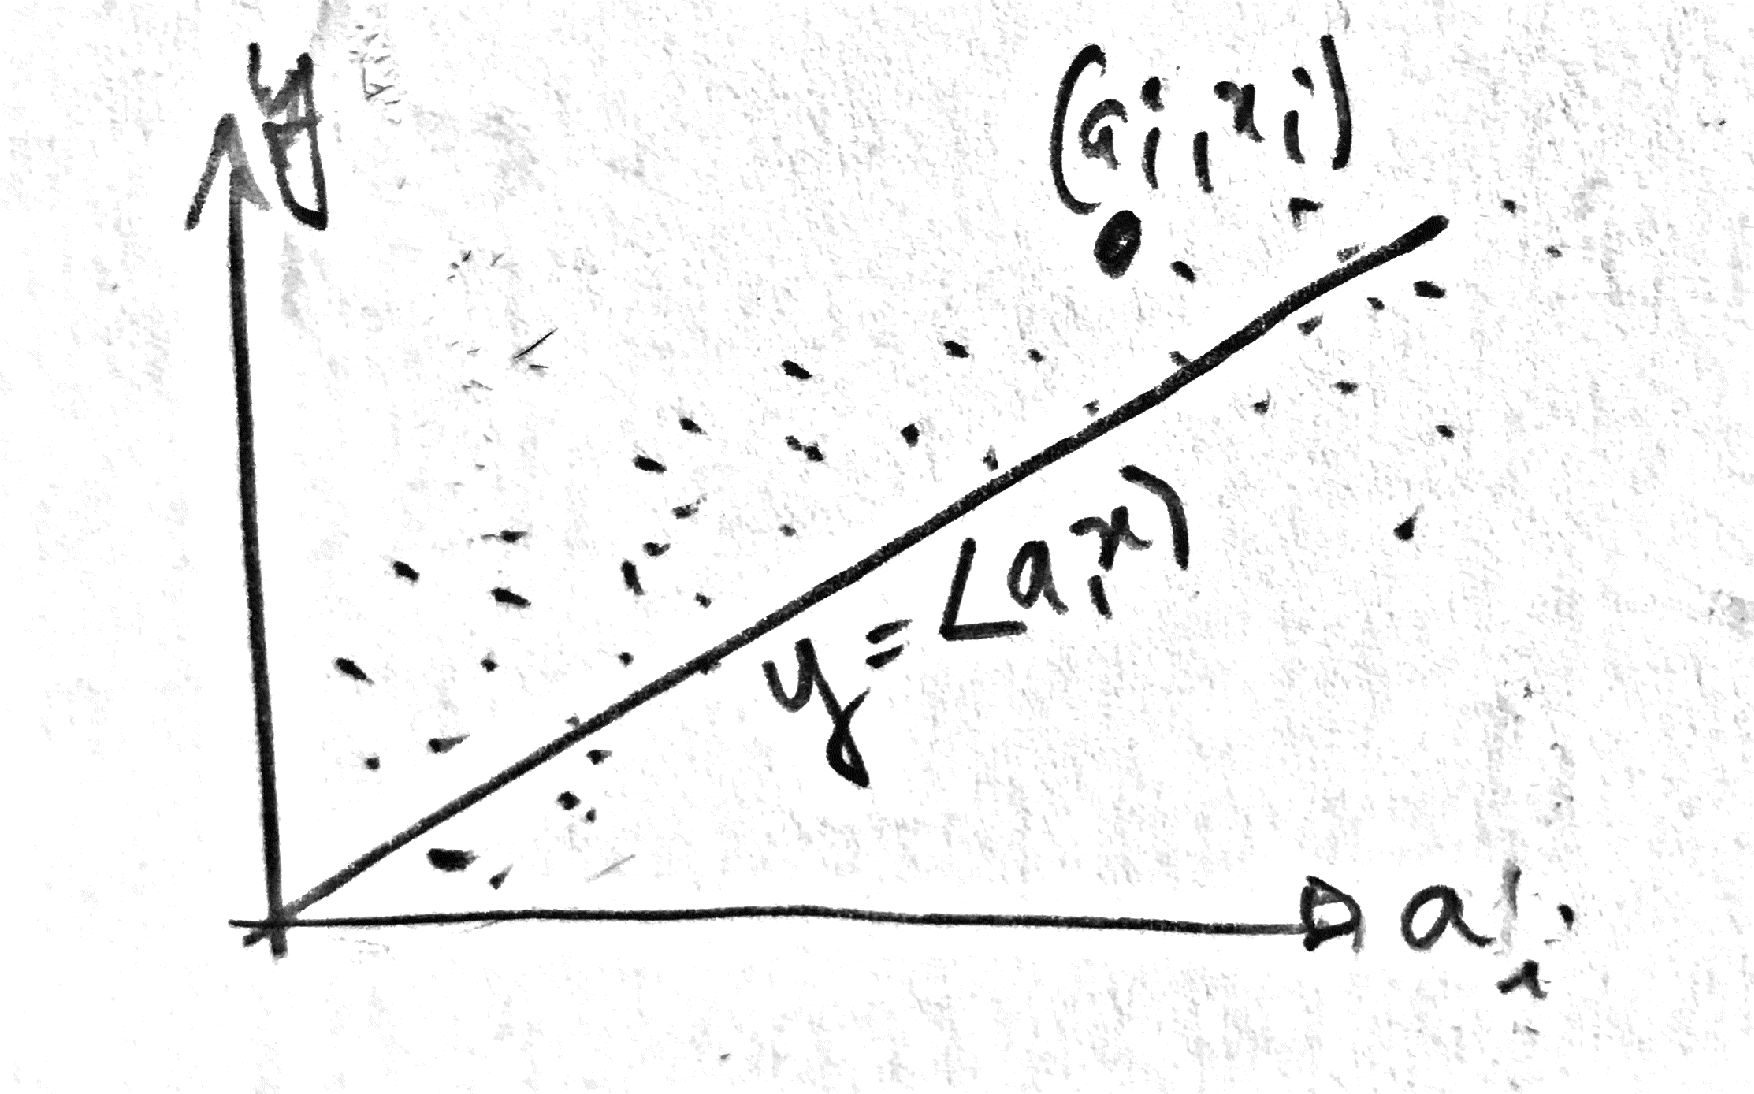
\includegraphics[width=.2\linewidth]{optim-smooth/ml-exemp-1} \quad
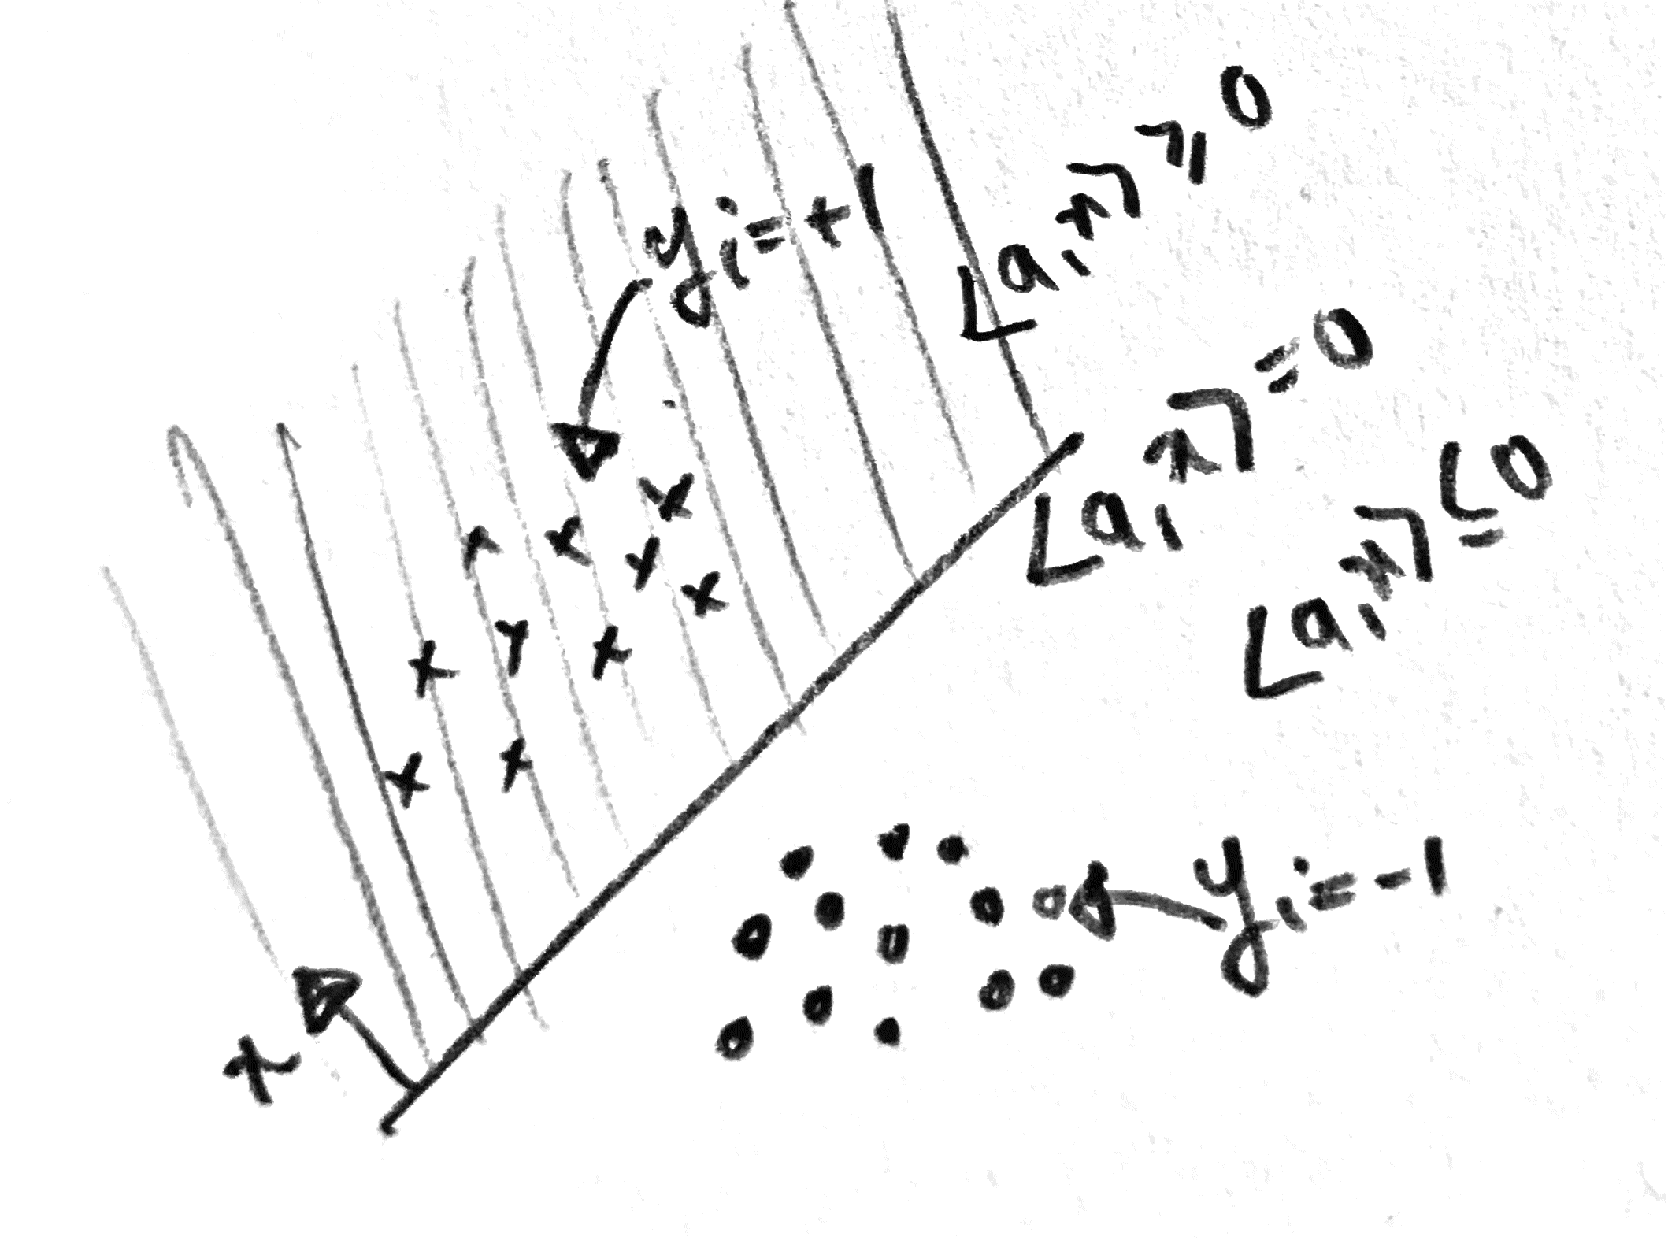
\includegraphics[width=.2\linewidth]{optim-smooth/ml-exemp-2} \quad
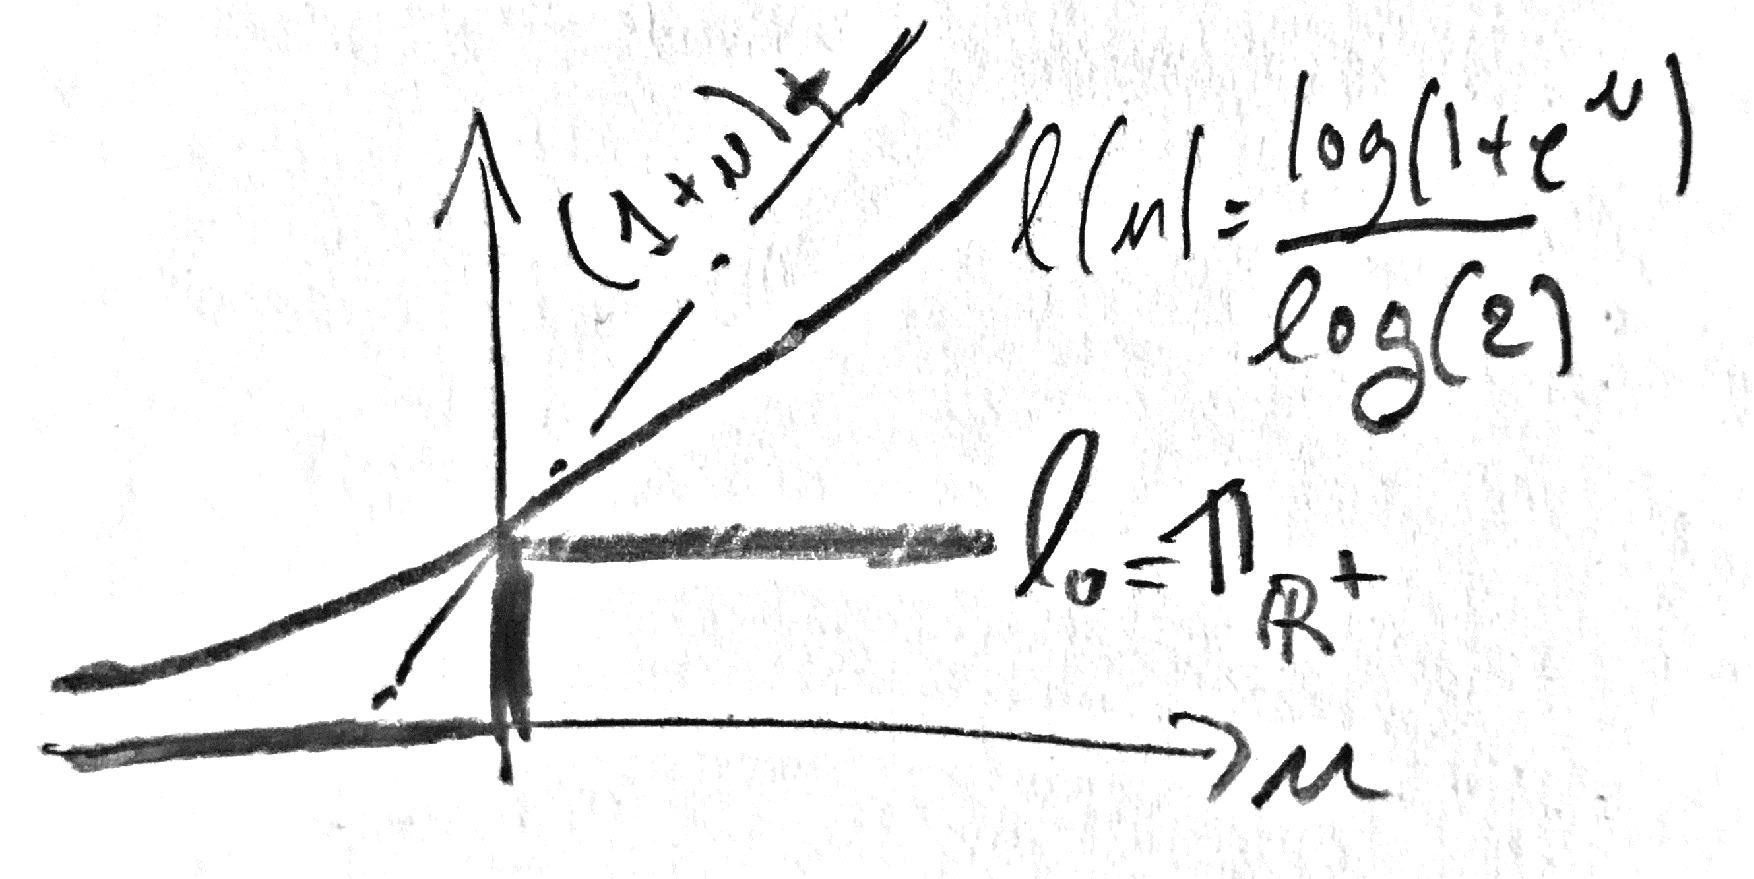
\includegraphics[width=.3\linewidth]{optim-smooth/classif-loss}
\caption{\label{fig-ml-ex}
Left: linear regression, middle: linear classifier, right: loss function for classification.
}
\end{figure}

\begin{exmp}[Regression]
For regression, $y_i \in \RR$, in which case
\eql{\label{eq-least-square}
	f(x) =  \frac{1}{2}\sum_{i=1}^n (y_i-\dotp{x}{a_i})^2 = \frac{1}{2}\norm{Ax-y}^2, 
} 
is the least square quadratic risk function (see Fig.~\ref{fig-ml-ex}).
%
Here $\dotp{u}{v}=\sum_{i=1}^p u_i v_i$ is the canonical inner product in $\RR^p$ and $\norm{\cdot}^2=\dotp{\cdot}{\cdot}$. 
\end{exmp}

\begin{exmp}[Classification]
For classification, $y_i \in \{-1,1\}$, in which case
\eql{\label{eq-classif}
	f(x) = \sum_{i=1}^n \ell(-y_i \dotp{x}{a_i}) = L( - \diag(y) A x )
}
where $\ell$ is a smooth approximation of the 0-1 loss $1_{\RR^+}$.
%
For instance $\ell(u)=\log(1+\exp(u))$, and $\diag(y) \in \RR^{n \times n}$ is the diagonal matrix with $y_i$ along the diagonal (see Fig.~\ref{fig-ml-ex}, right). Here the separable loss function $L = \RR^n \rightarrow \RR$ is, for $z \in \RR^n$, $L(z)=\sum_i \ell(z_i)$. 
\end{exmp}

%%%
\paragraph{Coercivity.}

In general, there might be no solution to the optimization~\eqref{eq-general-pbm}. This is of course the case if $f$ is unbounded by bellow, for instance $f(x)=-x^2$ in which case the value of the minimum is $-\infty$. But this might also happens if $f$ does not grow at infinity, for instance $f(x)=e^{-x}$, for which $\min f = 0$ but there is no minimizer.

In order to show existence of a minimizer, and that the set of minimizer is bounded (otherwise one can have problems with optimization algorithm that could escape to infinity), one needs to show that one can replace the whole space $\RR^p$ by a compact sub-set $\Om \subset \RR^p$ (i.e. $\Om$ is bounded and close) and that $f$ is continuous on $\Om$ (one can replace this by a weaker condition, that $f$ is lower-semi-continuous, but we ignore this here).  A way to show that one can consider only a bounded set is to show that $f(x) \rightarrow +\infty$ when $x \rightarrow +\infty$. Such a function is called coercive. In this case, one can choose any $x_0 \in \RR^p$ and consider its associated lower-level set
\eq{
	\Om = \enscond{x \in \RR^p}{f(x) \leq f(x_0)}
}
which is bounded because of coercivity, and closed because $f$ is continuous.

\begin{figure}
\centering
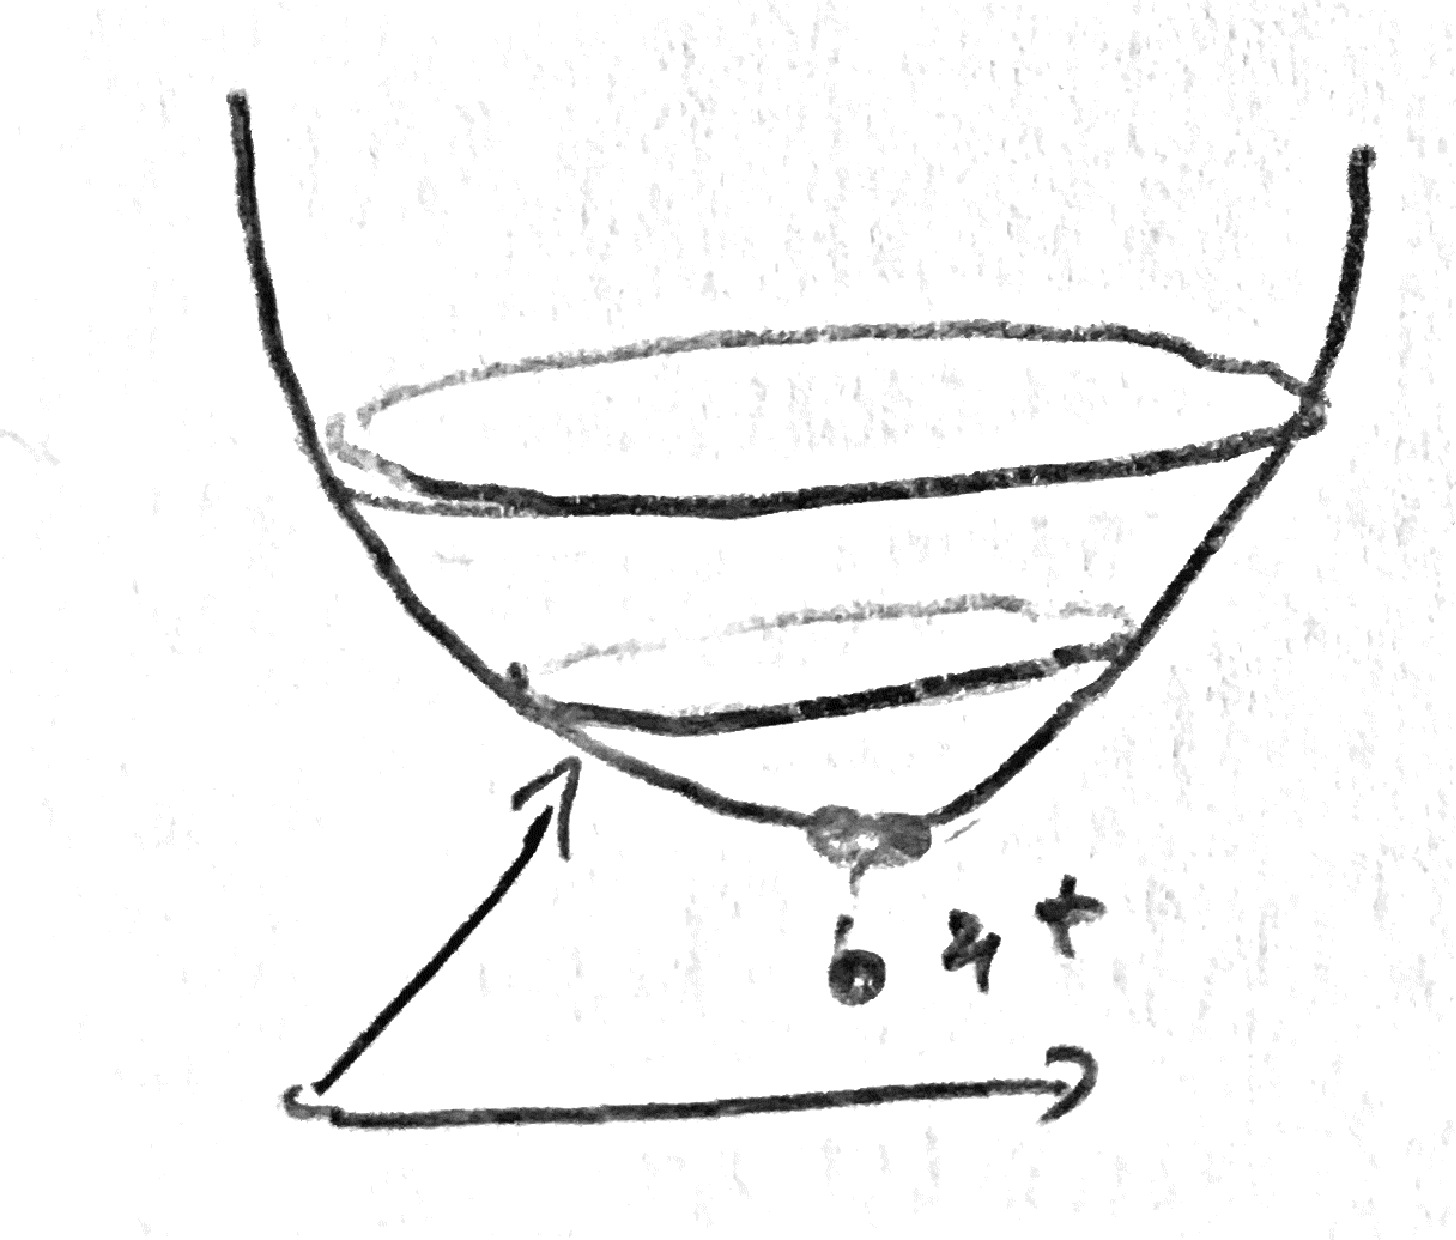
\includegraphics[width=.2\linewidth]{optim-smooth/least-square-1} \quad
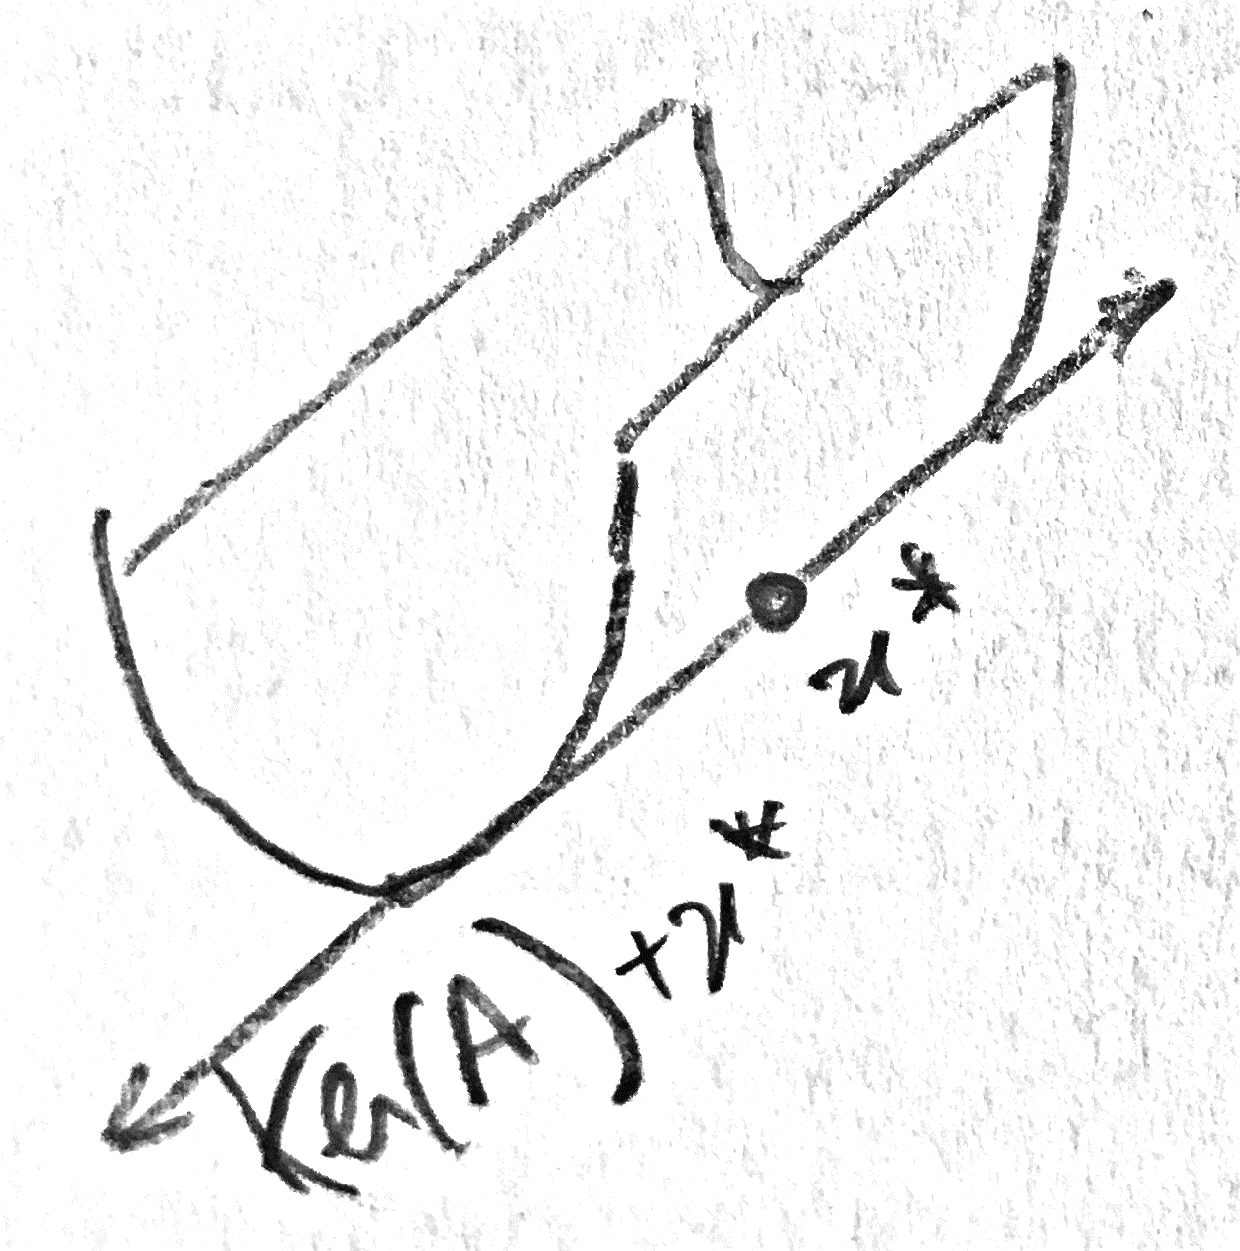
\includegraphics[width=.2\linewidth]{optim-smooth/least-square-2} 
\caption{\label{fig-least-square}
Coercivity condition for least squares.
}
\end{figure}

\begin{exmp}[Least squares]
For instance, for the quadratic loss function $f(x)=\frac{1}{2}\norm{Ax-y}^2$, coercivity holds if and only if $\ker(A)=\{0\}$ (this corresponds to the overdetermined setting). Indeed, if $\ker(A) \neq \{0\}$ if $x^\star$ is a solution, then $x^\star+u$ is also solution for any $u \in \ker(A)$, so that the set of minimizer is unbounded.
%
On contrary, if $\ker(A) = \{0\}$, we will show later that the set of minimizer is unique, see Fig.~\ref{fig-least-square}. 
%
If $\ell$ is strictly convex, the same conclusion holds in the case of classification.
\end{exmp}

%%%
\paragraph{Convexity.}

Convex functions define the main class of functions which are somehow ``simple'' to optimize, in the sense that all minimizers are global minimizers, and that there are often efficient methods to find these minimizers (at least for smooth convex functions). A convex function is such that for any pair of point $(x,y) \in (\RR^p)^2$, 
\eql{\label{eq-convexity-def}
	\foralls t \in [0,1], \quad
		f((1-t)x + t y) \leq (1-t)f(x) + t f(y)
}
which means that the function is bellow its secant (and actually also above its tangent when this is well defined), see Fig.~\ref{fig-cvx-vs-noncvx}. 
%
If $x^\star$ is a local minimizer of a convex $f$, then $x^\star$ is a global minimizer, i.e. $x^\star \in \argmin f$.  



Convex function are very convenient because they are stable under lots of transformation. In particular, if $f$, $g$ are convex and $a, b$ are positive, $a f + b g$ is convex (the set of convex function is itself an infinite dimensional convex cone!). If $g : \RR^q \rightarrow \RR$ is convex and $B \in \RR^{q \times p}, b \in \RR^q$ then $f(x) = g(B x+b)$ is convex. 
%
This shows immediately that the square loss appearing in~\eqref{eq-least-square} is convex, since $\norm{\cdot}^2/2$ is convex (as a sum of squares). 
%
Also, similarly, if $\ell$ and hence $L$ is convex, then the classification loss function~\eqref{eq-classif} is itself convex. 

\begin{figure}
\centering
\begin{tabular}{cccc}
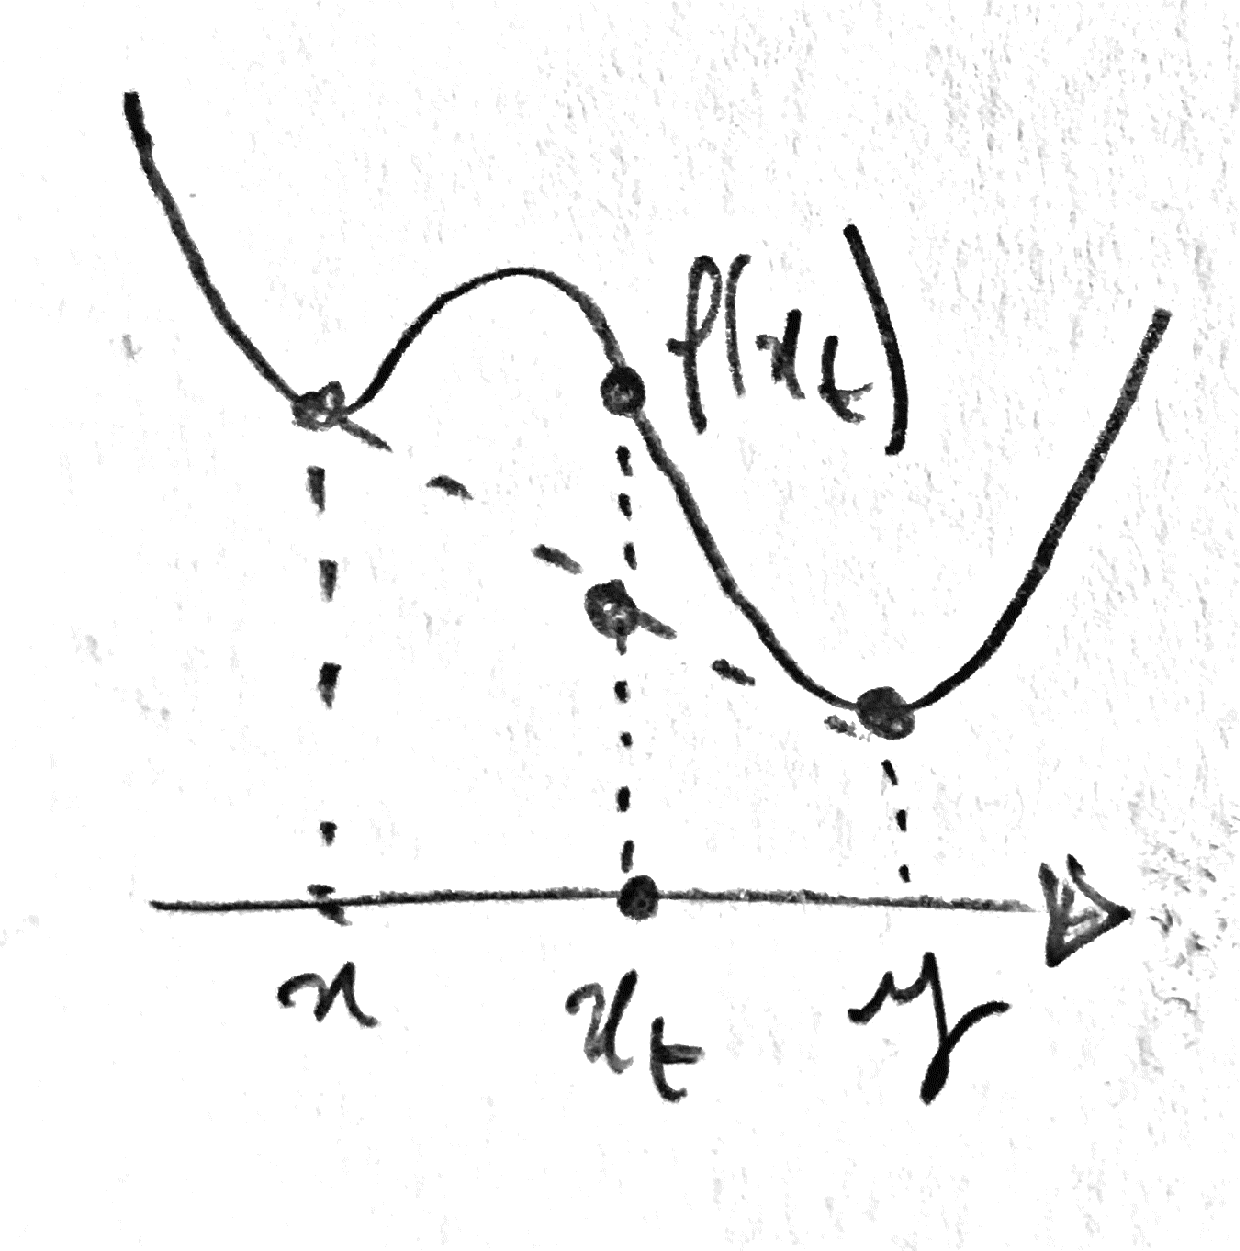
\includegraphics[width=.2\linewidth]{optim-smooth/cvx-vs-noncvx-1} &
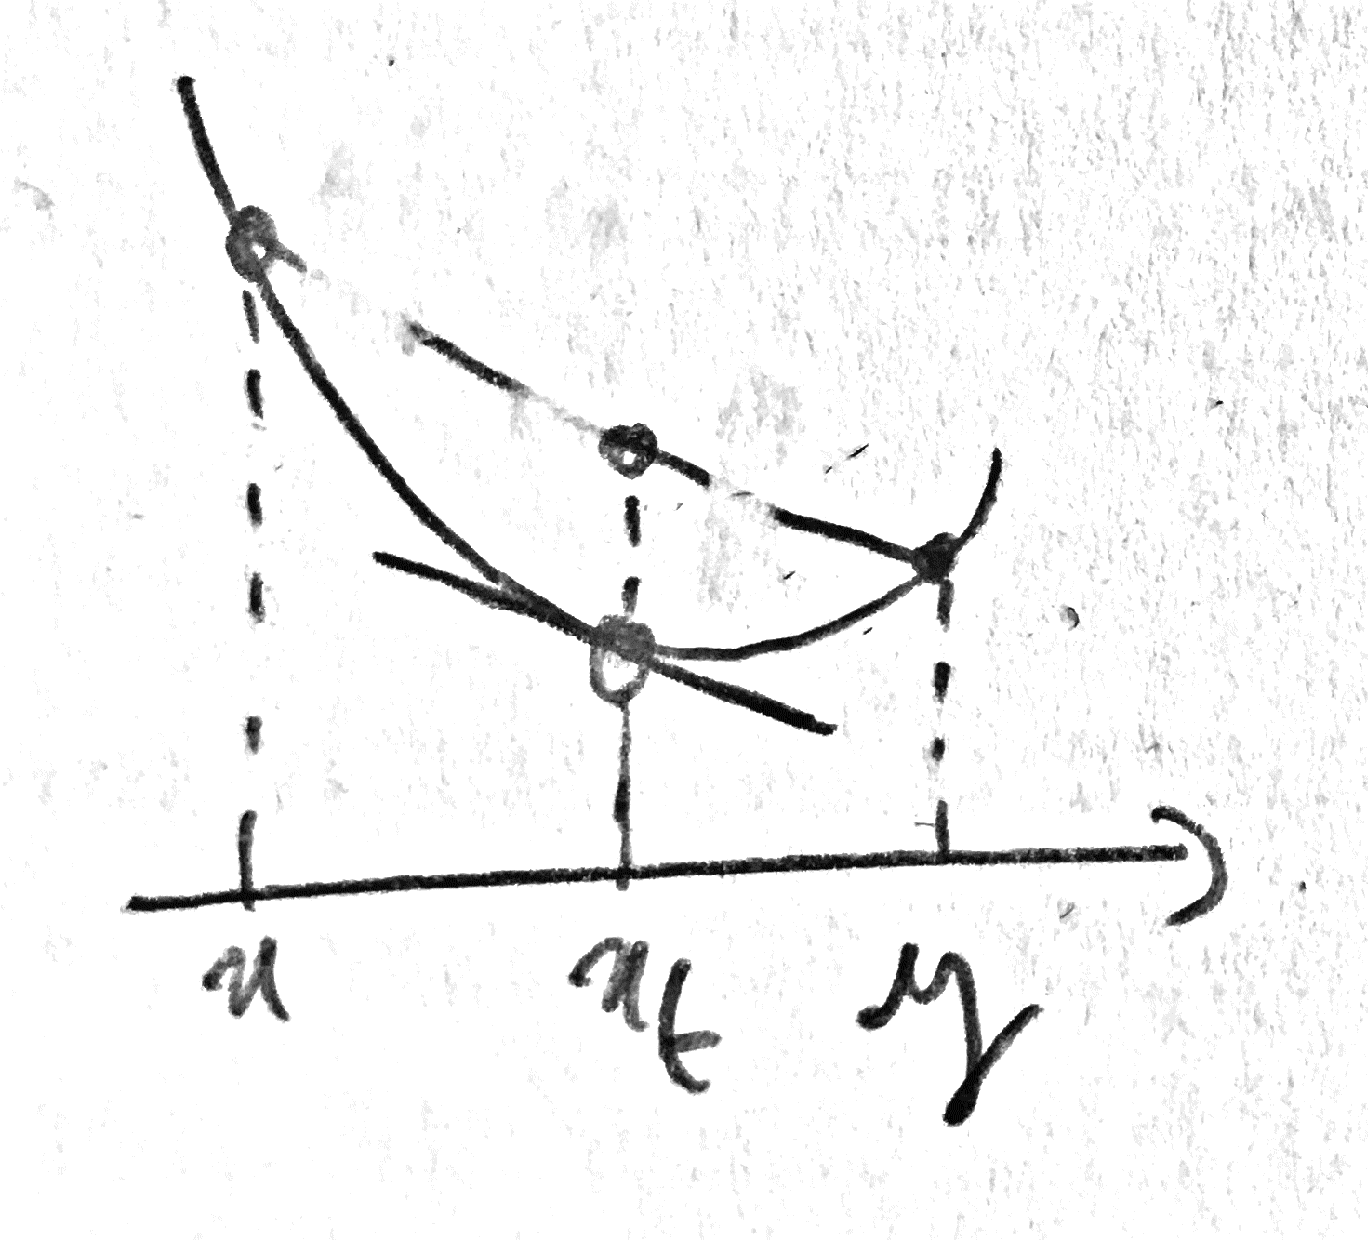
\includegraphics[width=.2\linewidth]{optim-smooth/cvx-vs-noncvx-2} &
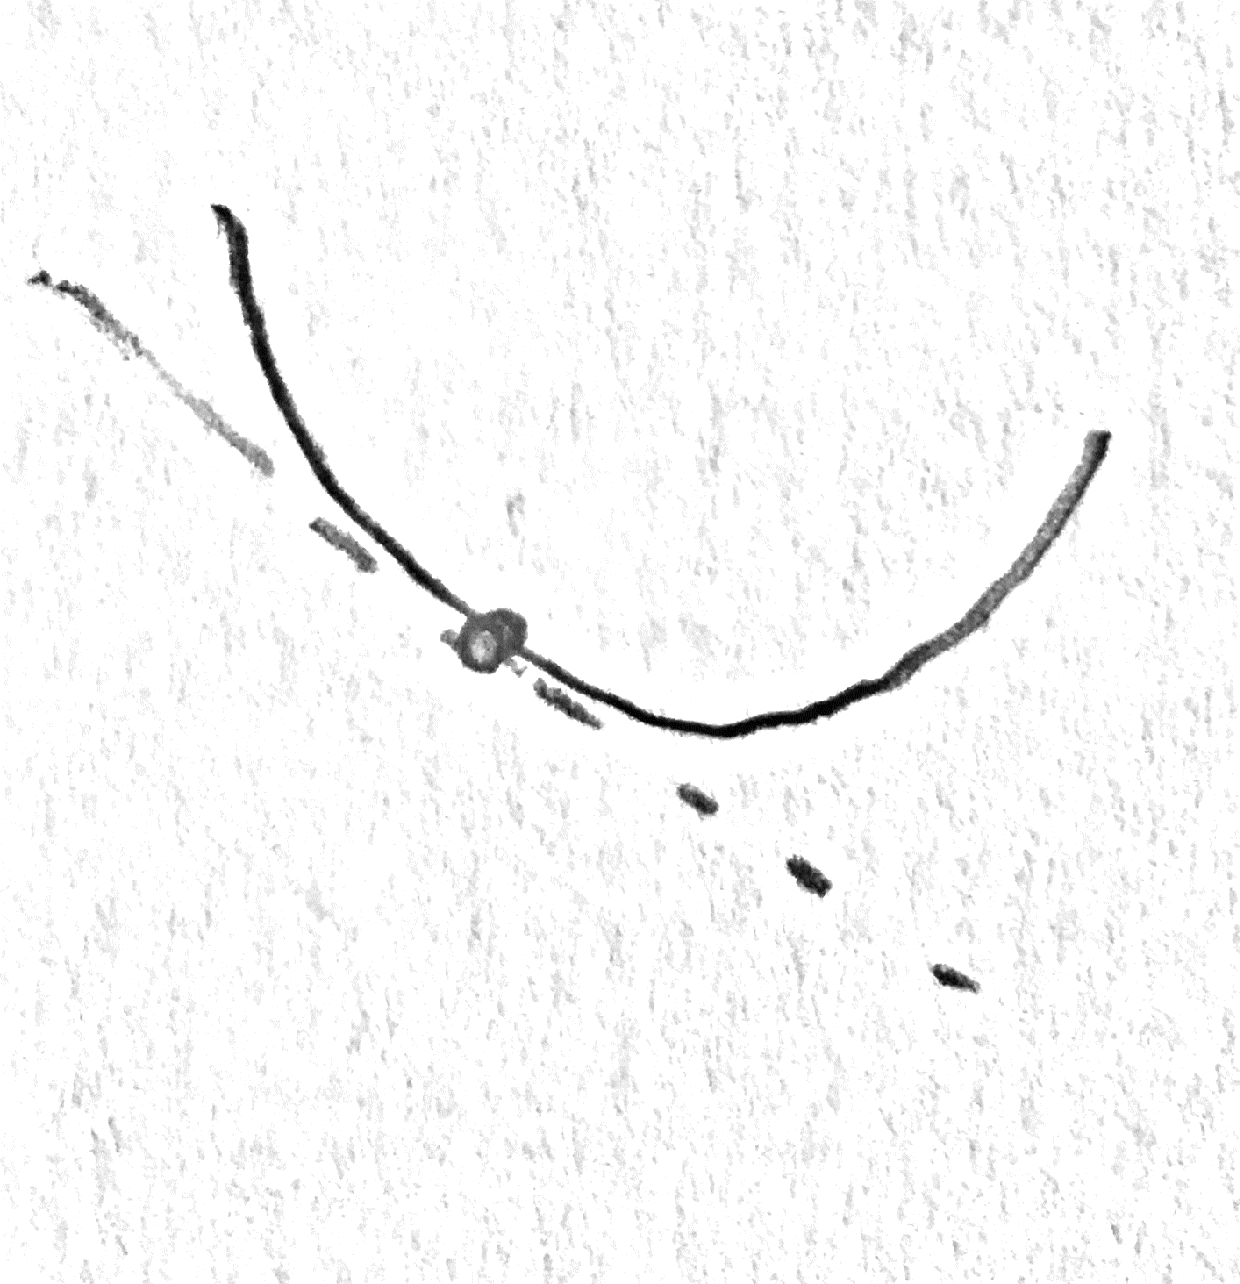
\includegraphics[width=.2\linewidth]{optim-smooth/strictly-cvx-2} &
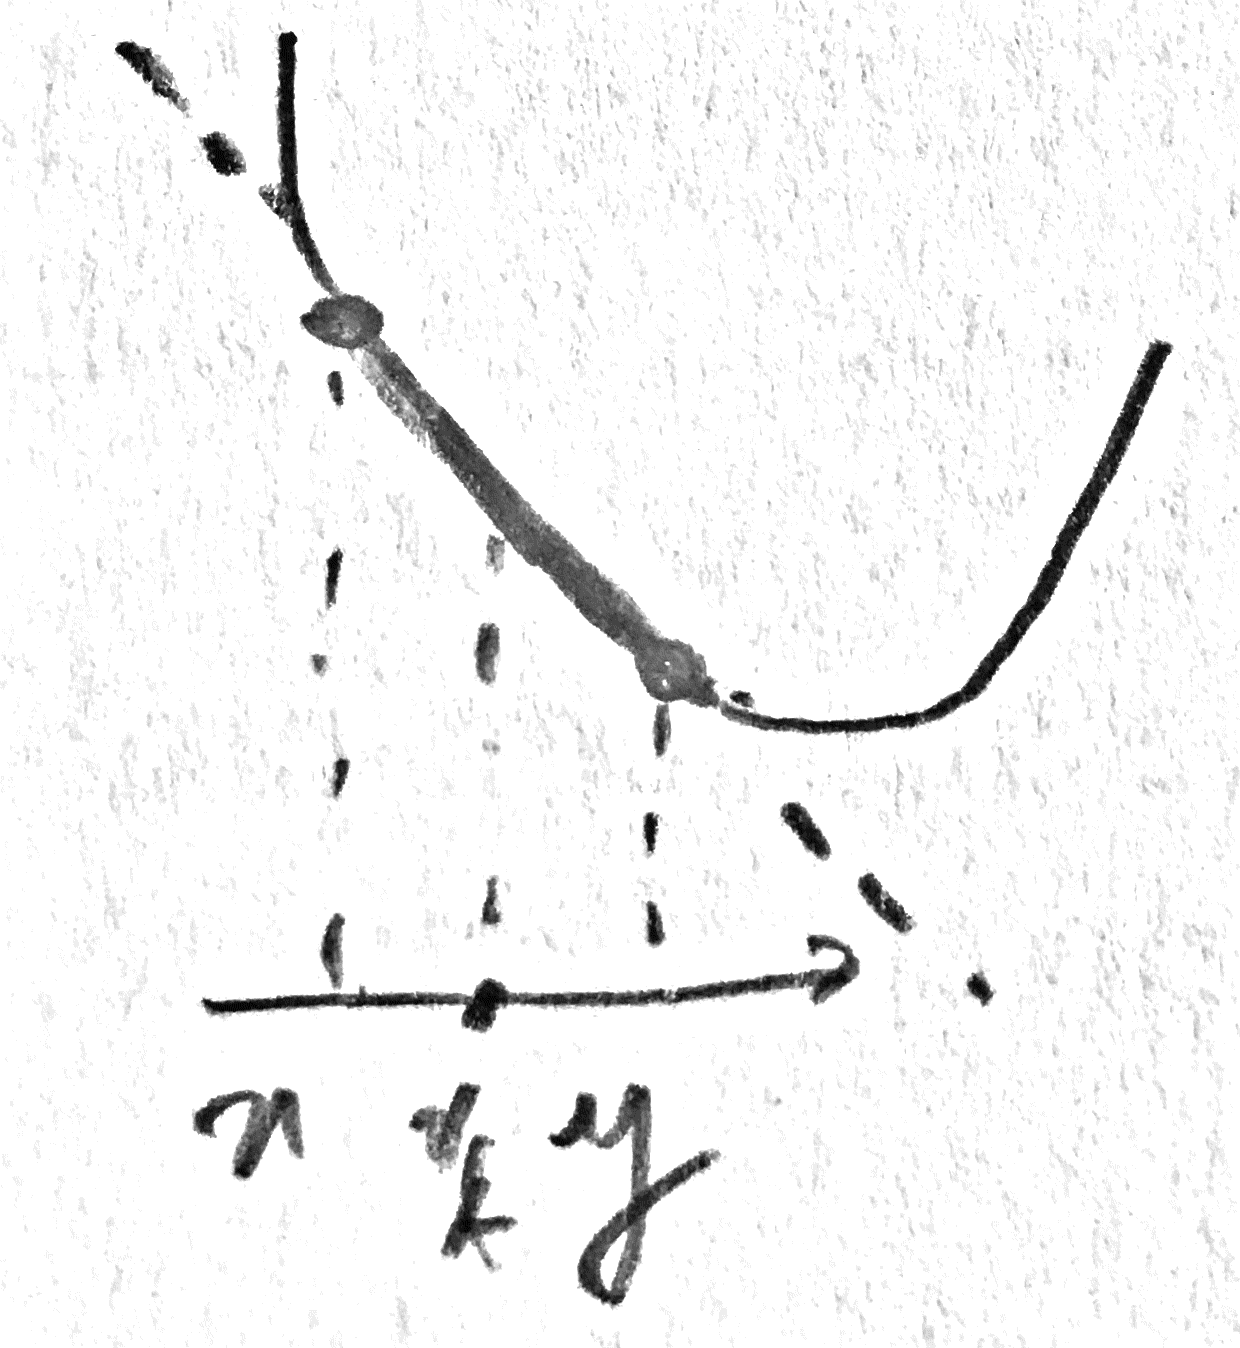
\includegraphics[width=.15\linewidth]{optim-smooth/strictly-cvx-1} 
\end{tabular}
\caption{\label{fig-cvx-vs-noncvx}
Convex vs. non-convex functions ; Strictly convex vs. non strictly convex functions.
}
\end{figure}


In general, minimizers $x^\star$ might be non-unique \todo{figure}. When $f$ is convex, one can strengthen the condition~\eqref{eq-convexity-def} and impose that the inequality is strict for $t \in ]0,1[$ (see Fig.~\ref{fig-cvx-vs-noncvx}, right), i.e.
\eql{\label{eq-strict-convexity-def}
	\foralls t \in ]0,1[, \quad
		f((1-t)x + t y) < (1-t)f(x) + t f(y).
}
In this case, if a minimum $x^\star$ exists, then it is unique.  Indeed, if $x_1^\star \neq x_2^\star$ were two different minimizer, one would have by strict convexity $f(\frac{x_1^\star+x_2^\star}{2}) < f(x_1^\star)$ which is impossible.


\begin{exmp}[Least squares]
	For the quadratic loss function $f(x)=\frac{1}{2}\norm{Ax-y}^2$, strict convexity is equivalent to $\ker(A)=\{0\}$ \todo{show this}.
\end{exmp}

%%%%%%%%%%%%%%%%%%%%%%%%%%%%%%%%%%%%%%%%%%%%%%%%%%%%%%%%%%%%%%%%%%%%%%%%%%%%%%%%%%
%%%%%%%%%%%%%%%%%%%%%%%%%%%%%%%%%%%%%%%%%%%%%%%%%%%%%%%%%%%%%%%%%%%%%%%%%%%%%%%%%%
%%%%%%%%%%%%%%%%%%%%%%%%%%%%%%%%%%%%%%%%%%%%%%%%%%%%%%%%%%%%%%%%%%%%%%%%%%%%%%%%%%
\section{Derivative and gradient}

%%%
\paragraph{Gradient.}


\wrapfSimple{optim-smooth/gradient-vector-field}
If $f$ is differentiable along each axis, we denote 
\eq{
	\nabla f(x) \eqdef ( \partial_{x_1} f(x), \ldots,\partial_{x_p} f(x) )^\top \in \RR^p
}
the gradient vector, so that $\nabla f : \RR^p \rightarrow \RR^p$ is a vector field.

Beware that $\nabla f(x)$ can exist without $f$ being differentiable. Differentiability of $f$ at each reads
\eql{\label{eq-grad-dfn}
	f(x+\epsilon) = f(x) + \dotp{\epsilon}{\nabla f(x)} + o(\norm{\epsilon}).
} 
%
Here $R(\epsilon) = o(\norm{\epsilon})$ denotes a quantity which decays faster than $\epsilon$ toward $0$, i.e. $\frac{R(\epsilon)}{\norm{\epsilon}} \rightarrow 0$ as $\epsilon \rightarrow 0$. Existence of partial derivative corresponds to $f$ being differentiable along the axes, while differentiability should hold for any converging sequence of $\epsilon\rightarrow 0$ (i.e. not along along a fixed direction). 

Also, $\nabla f(x)$ is the only vector such that the relation~\eqref{eq-grad-dfn}. This means that a possible strategy to both prove that $f$ is differentiable and to obtain a formula for $\nabla f(x)$ is to show a relation of the form 
\eq{
	f(x+\epsilon) = f(x) + \dotp{\epsilon}{g} + o(\norm{\epsilon}), 
}
in which case one necessarily has $\nabla f(x)=g$. 


%%%
\paragraph{First order condition.}

The main theoretical interest (we will see later that it also have algorithmic interest) of the gradient vector is that it is a nessarily condition for optimality, as stated bellow. 

\begin{prop} 
If $x^\star$ is a local minimum of the function $f$ (i.e. that $f(x^\star) \leq f(x)$ for all $x$ in some ball around $x^\star$) then 
\eq{
	\nabla f(x^\star) = 0. 
} 
\end{prop}
\begin{proof}
One has for $\epsilon$ small enough and $u$ fixed 
\eq{
	f(x^\star) \leq f(x^\star+\epsilon u) = f(x^\star) + \epsilon \dotp{\nabla f(x^\star)}{u} + o(\epsilon) 
	\qarrq
	\dotp{\nabla f(x^\star)}{u} \geq o(1)
	\qarrq
	\dotp{\nabla f(x^\star)}{u} \geq 0.
}	
So applying this for $u$ and $-u$ in the previous equation shows that $\dotp{\nabla f(x^\star)}{u}=0$ for all $u$, and hence $\nabla f(x^\star)=0$.
\end{proof}

Note that the converse is not true in general, since one might have $\nabla f(x)=0$ but $x$ is not a local mininimum. For instance $x=0$ for $f(x)=-x^2$ (here $x$ is a maximizer) or $f(x)=x^3$ (here $x$ is neither a maximizer or a minimizer, it is a saddle point), see Fig.~\ref{fig-first-order}. 
%
Note however that in practice, if $\nabla f(x^\star) = 0$ but $x$ is not a local minimum, then $x^\star$ tends to be an unstable equilibrium. Thus most often gradient-based algorithm will converge to point with $\nabla f(x^\star) = 0$ that are local minimizer.
%
The following proposition shows that a much strong result holds if $f$ is convex.

\begin{figure}
\centering
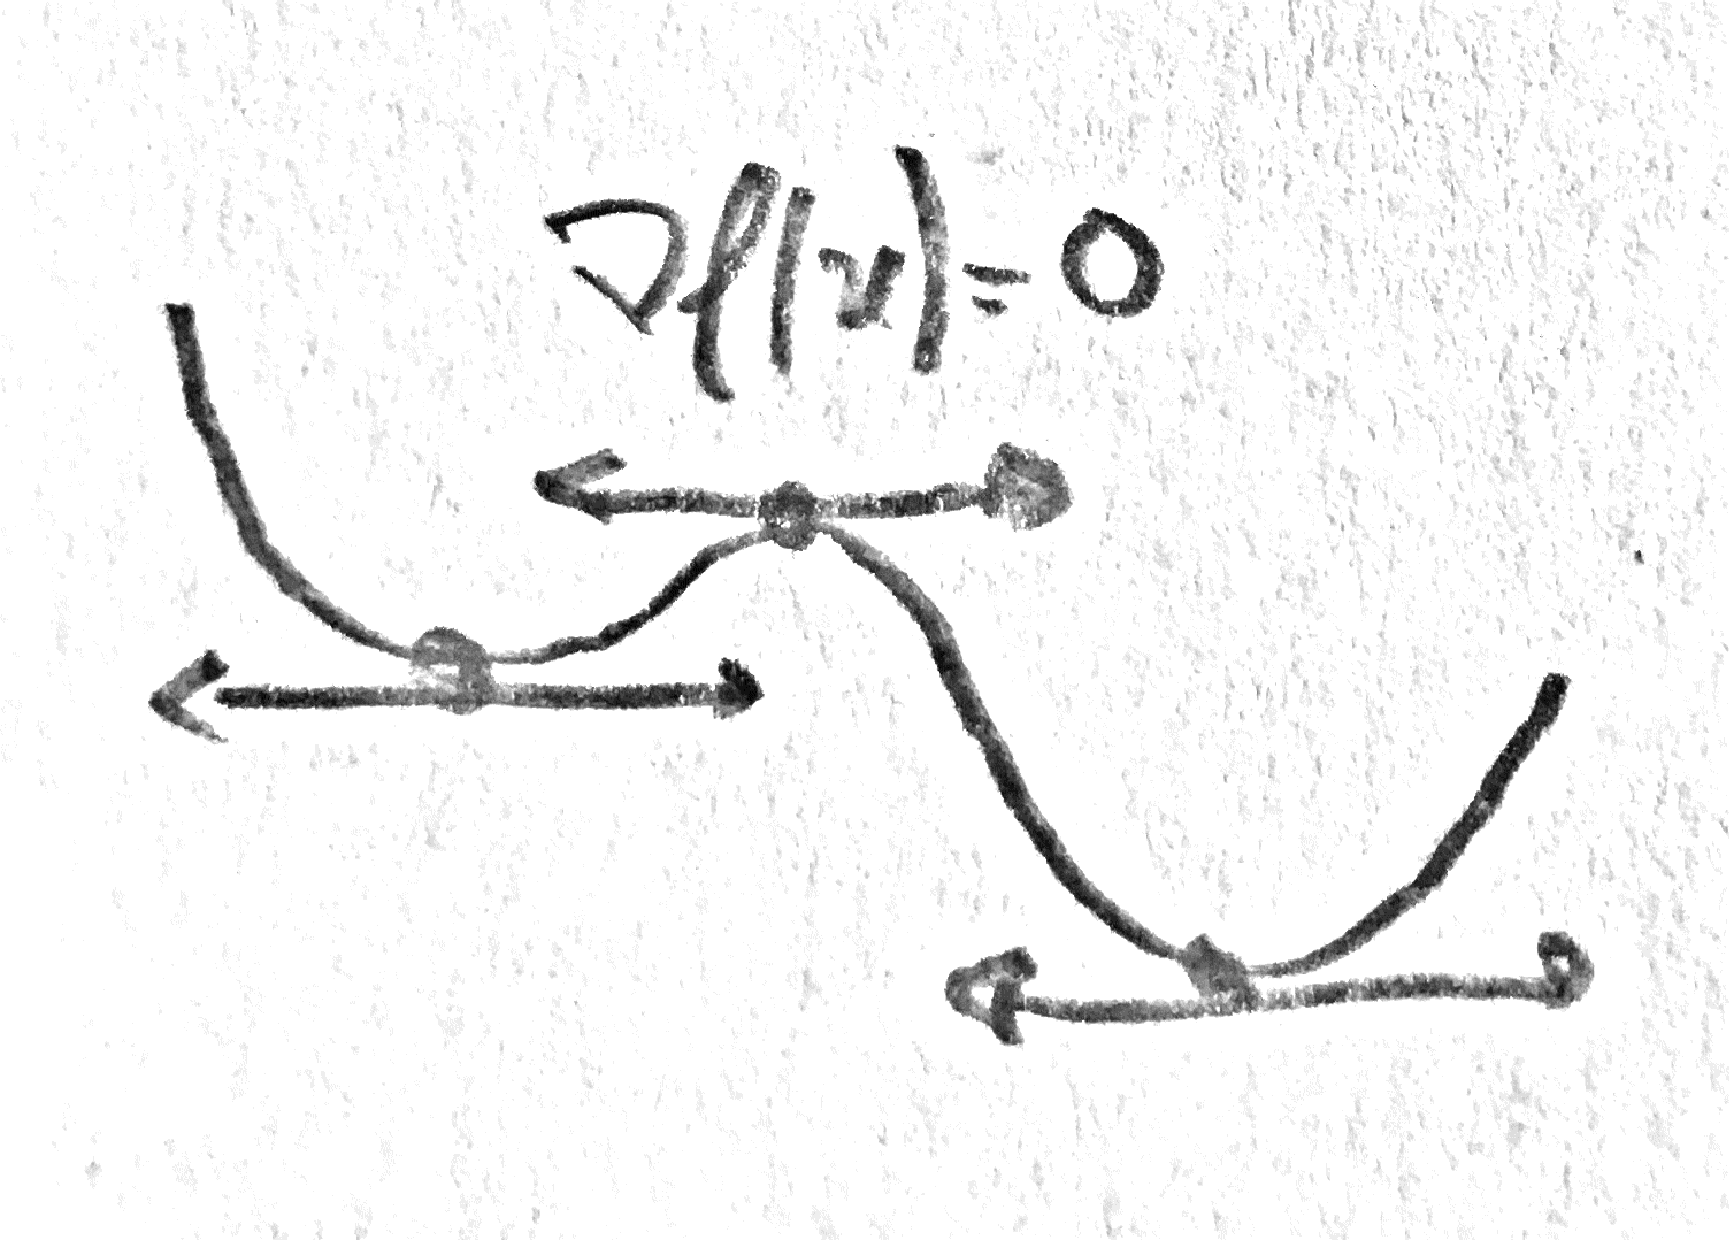
\includegraphics[width=.2\linewidth]{optim-smooth/first-order-1} \quad
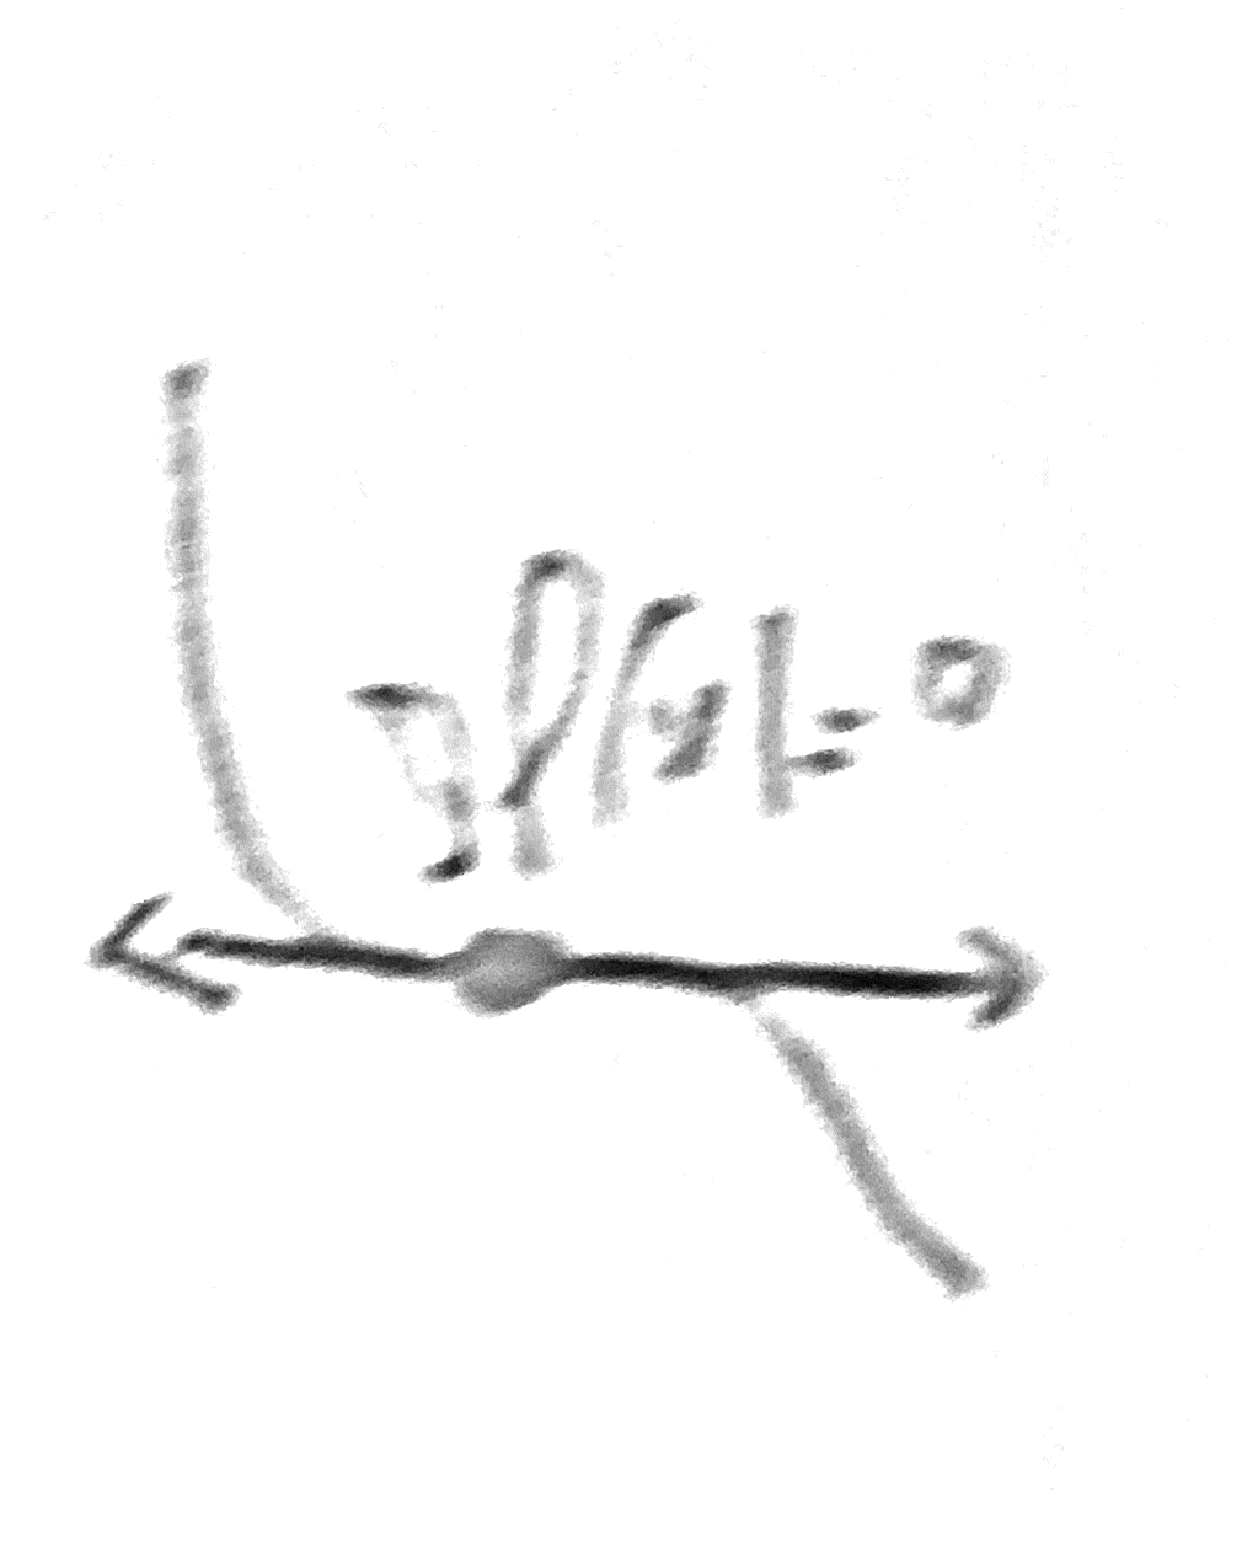
\includegraphics[width=.15\linewidth]{optim-smooth/first-order-2} \quad
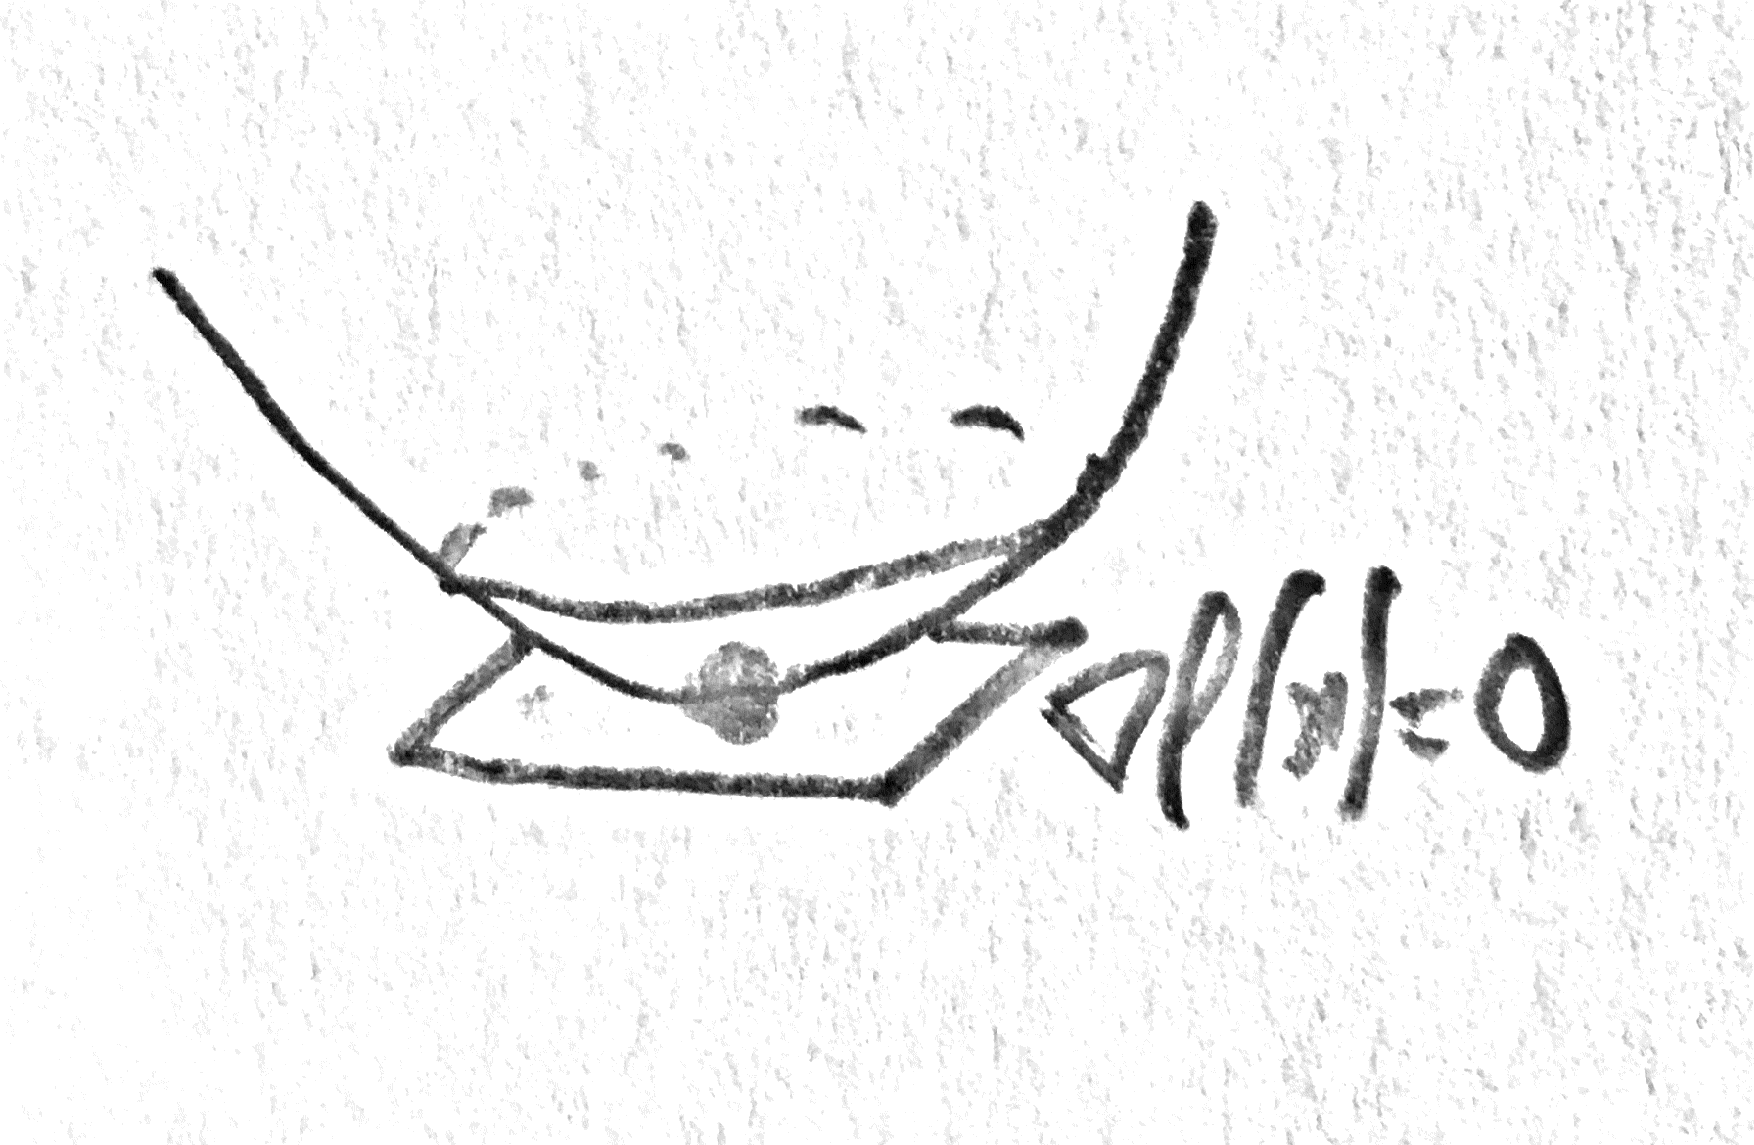
\includegraphics[width=.2\linewidth]{optim-smooth/first-order-3} 
\caption{\label{fig-first-order}
Function with local maxima/minima (left),  saddle point (middle) and global minimum (right). 
}
\end{figure}


\begin{prop} 
If $f$ is differentiable and convex, 
\eq{
	x^\star \in \uargmin{x} f(x) 
	\quad\Longleftrightarrow\quad
	\nabla f(x^\star)=0.
}
\end{prop}
\begin{proof}
\todo{write me}
\end{proof}

Thus in this case, optimizing a function is the same a solving an equation $\nabla f(x)=0$ (actually $p$ equations in $p$ unknown).
%
In most case it is impossible to solve this equation, but it often provides interesting information about solutions $x^\star$.


%%%
\paragraph{Example: Least squares.}

The most important gradient formula is the one of the square loss~\eqref{eq-least-square}, which can be obtained by expanding the norm
\begin{align*}
	f(x+\epsilon) &= \frac{1}{2}\norm{Ax-y+A\epsilon}^2 = \frac{1}{2}\norm{Ax-y} + \dotp{Ax-y}{A\epsilon} + \frac{1}{2}\norm{A\epsilon}^2 \\
		&=f(x) + \dotp{\epsilon}{A^\top(Ax-y)} + o(\norm{\epsilon}).
\end{align*} 
Here, we have used the fact that $\norm{A\epsilon}^2 = o(\norm{\epsilon})$ and use the transpose matrix $A^\top$. 
%
This matrix is obtained by exchanging the rows and the columns, i.e. $A^\top = (A_{j,i})_{i=1,\ldots,n}^{j=1,\ldots,p}$, but the way it should be remember and used is that it obeys the following swapping rule of the inner product, 
\eq{
	\foralls (u,v) \in \RR^{p} \times \RR^n, \quad
	\dotp{A u}{v}_{\RR^n} = \dotp{u}{A^\top v}_{\RR^p}. 
}
Computing gradient for function involving linear operator will necessarily requires such a transposition step.
%
This computation shows that
\eq{
	\nabla f(x) = A^\top (A x - y). 
}
This implies that solutions $x^\star$ minimizing $f(x)$ satisfies the linear system $(A^\top A) x^\star = A^\top y$. 
%
If $A^\star A \in \RR^{p \times p}$ is invertible, then $f$ has a single minimizer, namely  
\eql{\label{eq-sol-leastsquare}
	x^\star = (A^\top A)^{-1} A^\top y.
}
This shows that in this case, $x^\star$ depends linearly on the data $y$, and the corresponding linear operator $(A^\top A)^{-1} A^\star$ is often called the Moore-Penrose pseudo-inverse of $A$ (which is not invertible in general, since typically $p \neq n$). 
%
The condition that $A^\top A$ is invertible is equivalent to $\ker(A)=\{0\}$, since 
\eq{
	A^\top A x = 0 \qarrq \norm{Ax}^2 = \dotp{A^\top A x}{x} = 0 \qarrq A x= 0.
}
In particular, if $n<p$ (under-determined regime, there is too much parameter or too few data) this can never holds. If $n \geq p$ and the features $x_i$ are ``random'' then $\ker(A)=\{0\}$ with probability one. In this overdetermined situation $n \geq p$,  $\ker(A)=\{0\}$ only holds if the features $\{a_i\}_{i=1}^n$ spans a linear space $\Im(A^\top)$ of dimension strictly smaller than the ambient dimension $p$. 

%%%
\paragraph{Example: Classification}

We can do a similar computation for the gradient of the classification loss~\eqref{eq-classif}. Assuming that $L$ is differentiable, and using the Taylor expansion~\eqref{eq-grad-dfn} at point $-\diag(y) Ax$, one has 
\begin{align*}
	f(x+\epsilon) &= L( -\diag(y) Ax -\diag(y)  A\epsilon) \\
	&= L(-\diag(y) Ax) + \dotp{\nabla L( -\diag(y) Ax)}{ -\diag(y)  A\epsilon } + o(\norm{\diag(y)  A\epsilon})
\end{align*} 
Using the fact that $o(\norm{\diag(y)  A\epsilon}) = o(\norm{\epsilon})$, one obtains
\begin{align*}
	f(x+\epsilon) &= f(x) + \dotp{\nabla L( -\diag(y) Ax)}{-\diag(y)  A\epsilon} + o(\norm{\epsilon}) \\
		 &=  f(x) + \dotp{-A^\top \diag(y) \nabla L( -\diag(y) Ax)}{\epsilon} + o(\norm{\epsilon}), 
\end{align*} 	
where we have used the fact that $(AB)^\top = B^\top A^\top$ and that $\diag(y)^\top=\diag(y)$. This shows that
\eq{
	\nabla f(x) = -A^\top \diag(y) \nabla L( -\diag(y) Ax). 
}
Since $L(z) = \sum_i \ell(z_i)$, one has $\nabla L(z) = (\ell'(z_i))_{i=1}^n$. For instance, for the logistic classification method, $\ell(u) = \log(1+\exp(u))$ so that $\ell'(u) = \frac{e^u}{1+e^u} \in [0,1]$ (which can be interpreted as a probability of predicting $+1$).


%%%%%%%%%%%%%%%%%%%%%%%%%%%%%%%%%%%%%%%%%%%%%%%%%%%%%%%%%%%%%%%%%%%%%%%%%%%%%%%%%%
%%%%%%%%%%%%%%%%%%%%%%%%%%%%%%%%%%%%%%%%%%%%%%%%%%%%%%%%%%%%%%%%%%%%%%%%%%%%%%%%%%
%%%%%%%%%%%%%%%%%%%%%%%%%%%%%%%%%%%%%%%%%%%%%%%%%%%%%%%%%%%%%%%%%%%%%%%%%%%%%%%%%%
\section{Gradient Descent}


%%%
\paragraph{Steepest descent direction.}

The Taylor expansion~\eqref{eq-grad-dfn} computes an affine approximation of the function $f$ near $x$, since it can be written as
\eq{
	f(z) = T_x(z) + o(\norm{x-z})
	\qwhereq
	T_x(z) \eqdef f(x) + \dotp{\nabla f(x)}{z-x}, 
}
see Fig.~\ref{fig-expansion-taylor}. First order methods operate by locally replacing $f$ by $T_x$.


\begin{figure}
\centering
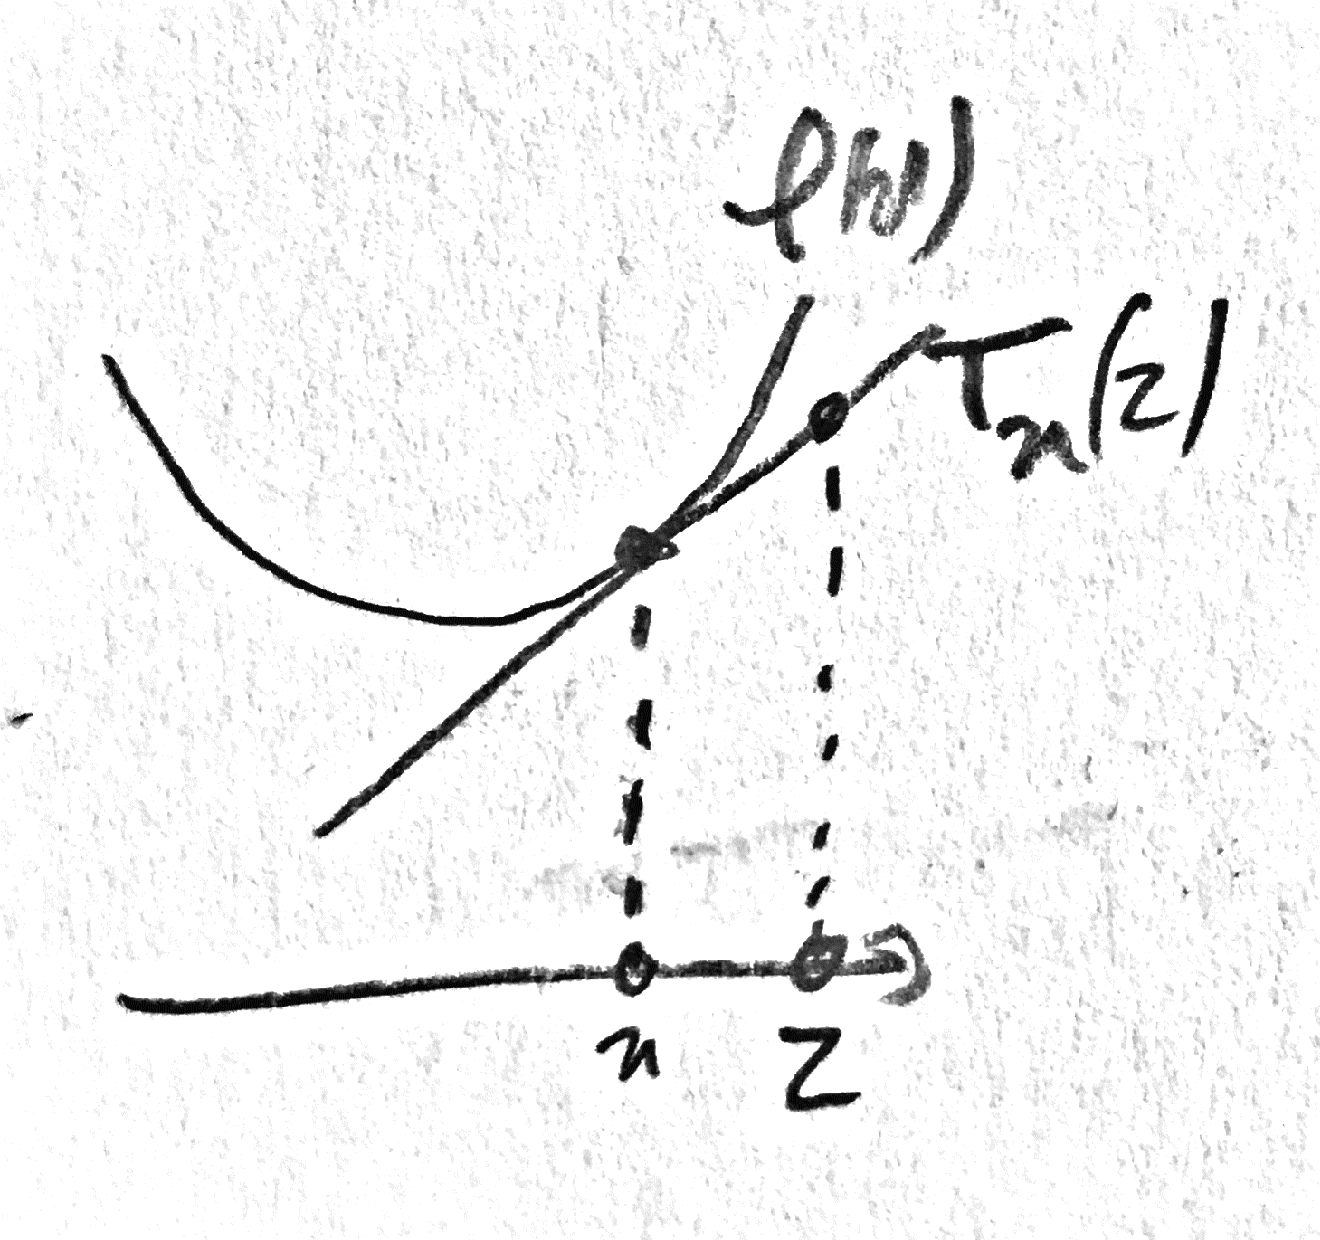
\includegraphics[width=.2\linewidth]{optim-smooth/taylor-exp-1} \quad
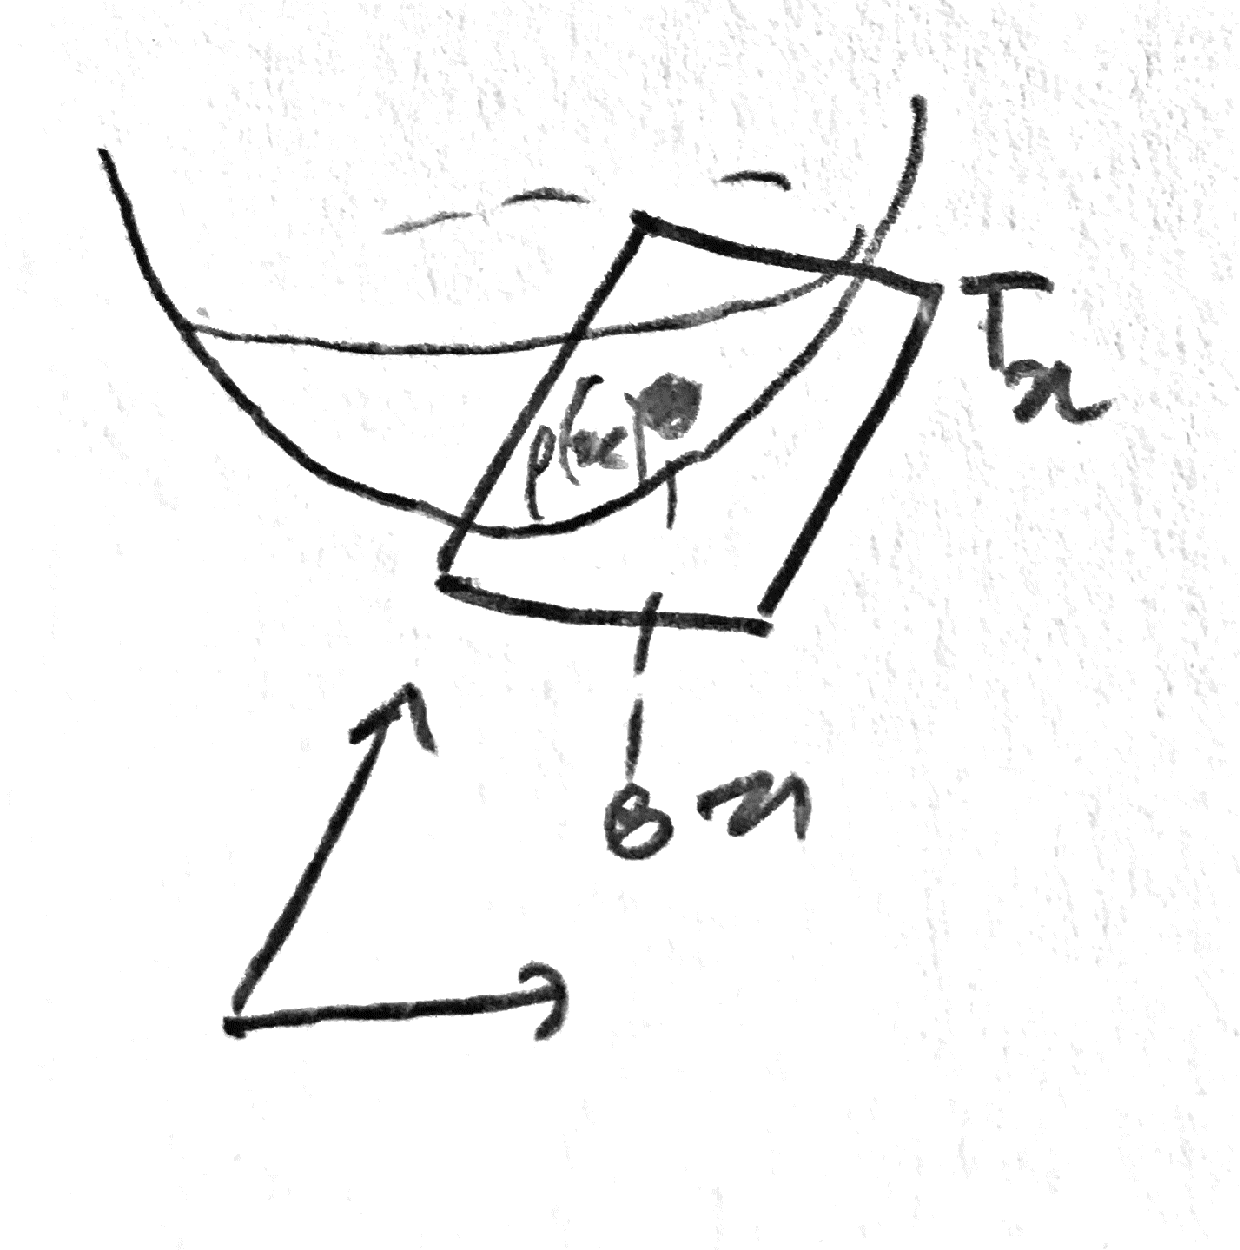
\includegraphics[width=.18\linewidth]{optim-smooth/taylor-exp-2} \quad
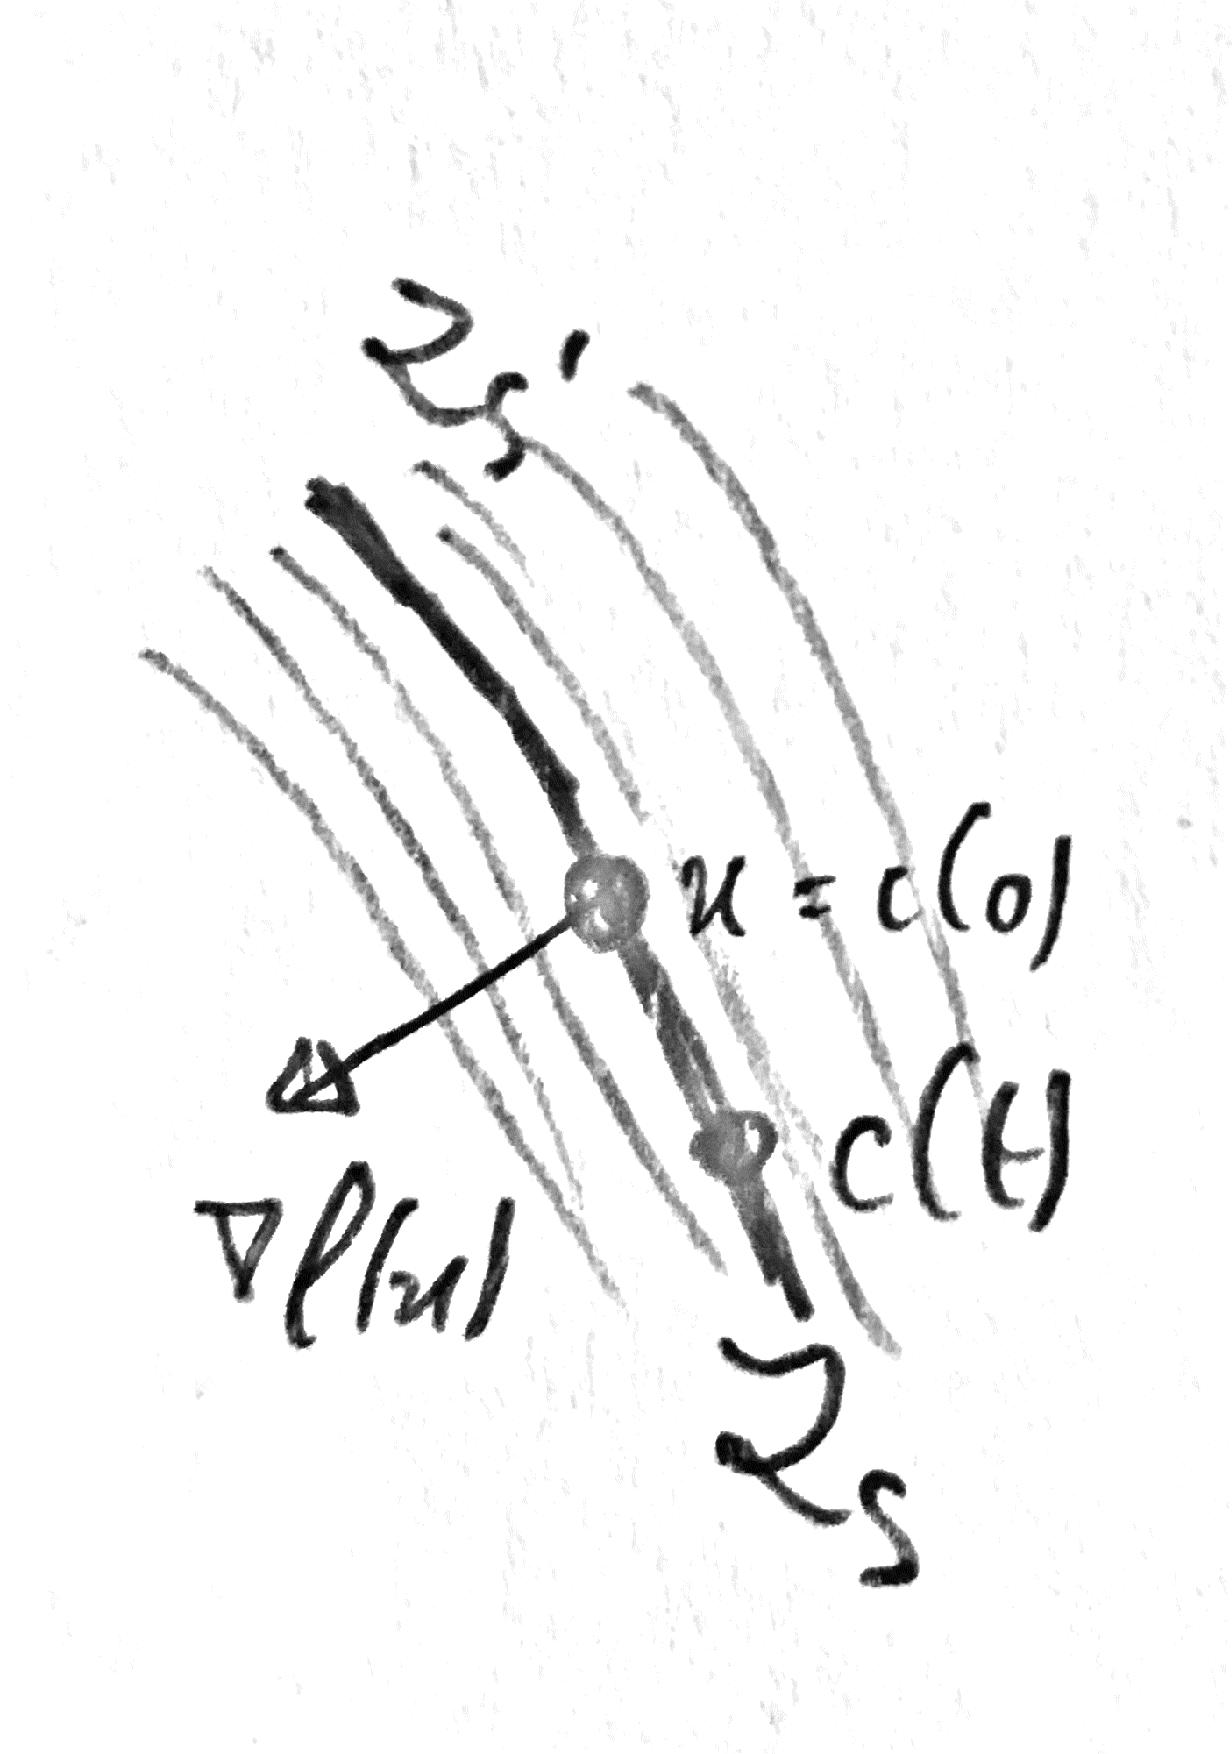
\includegraphics[width=.18\linewidth]{optim-smooth/level-sets-1} \quad
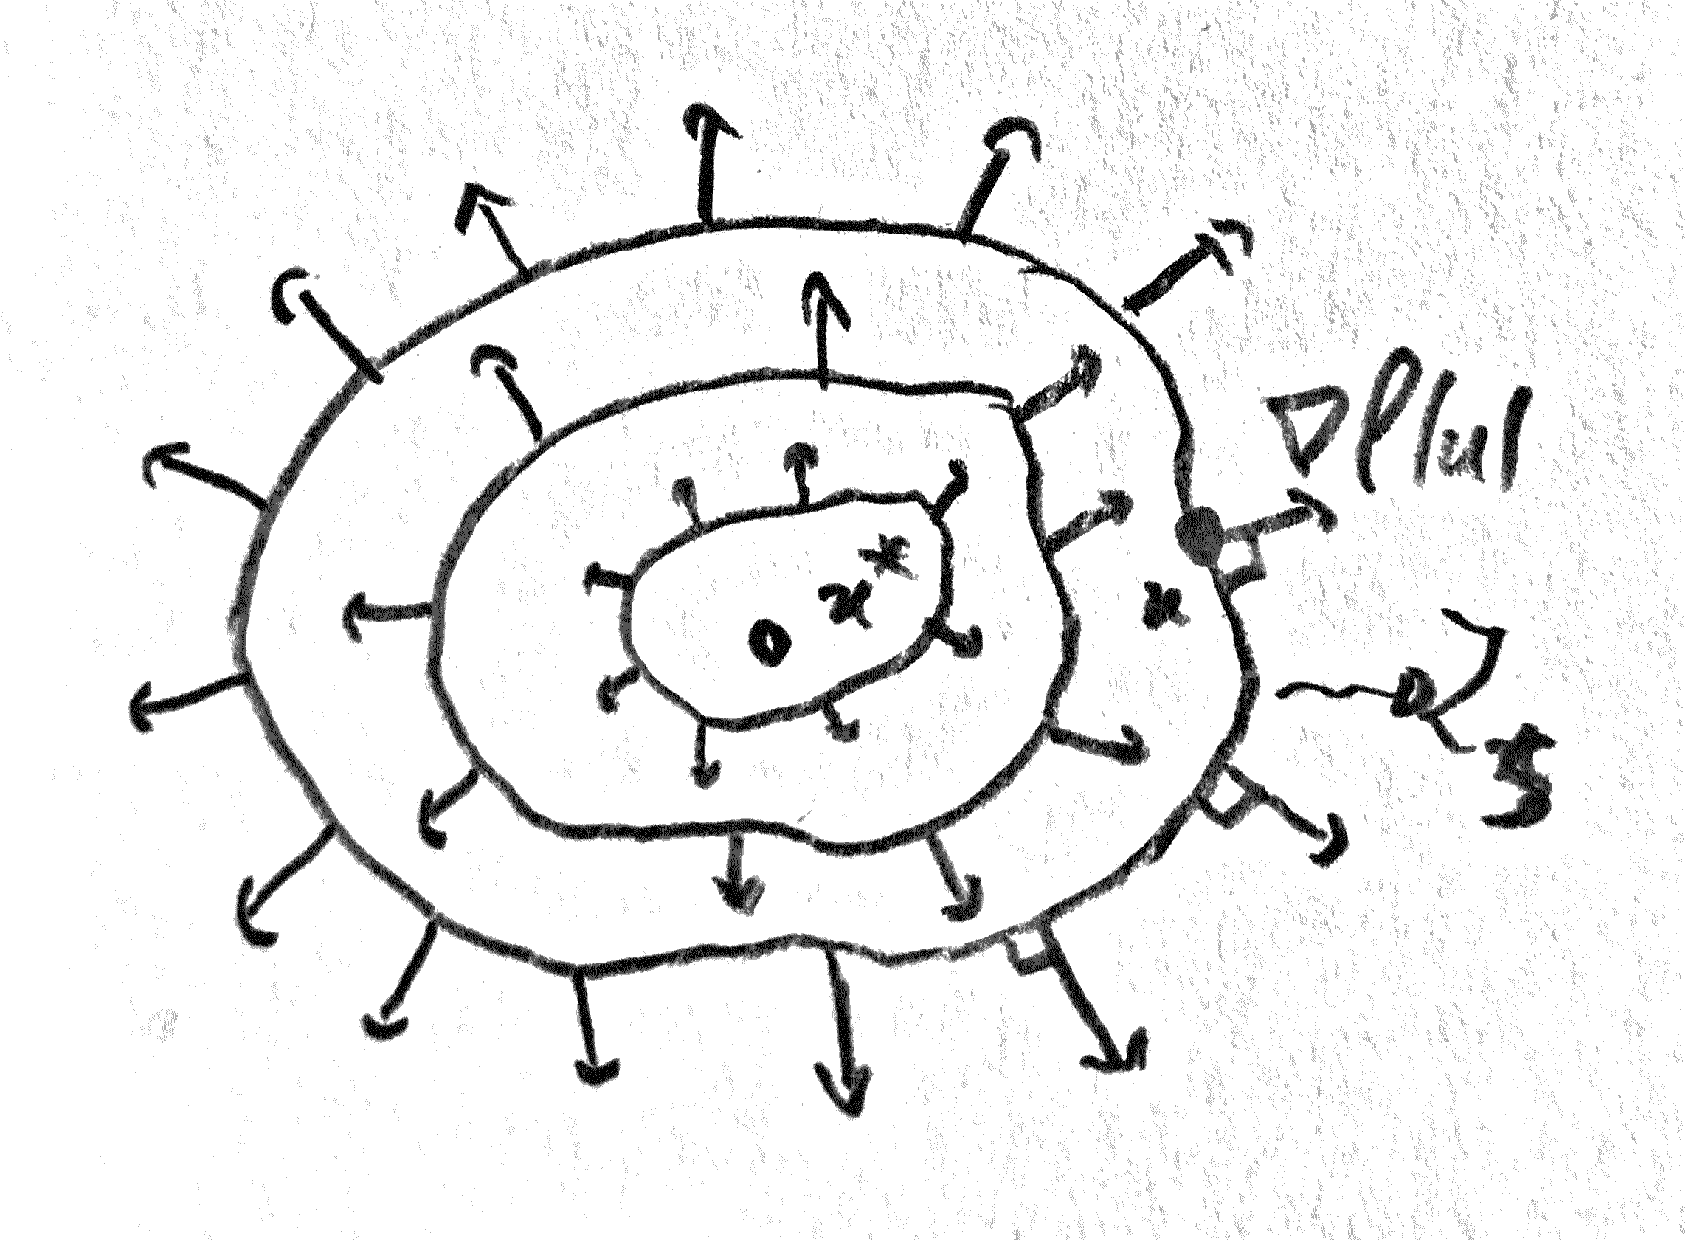
\includegraphics[width=.25\linewidth]{optim-smooth/level-sets-2} 
\caption{\label{fig-expansion-taylor}
	Left: First order Taylor expansion in 1-D and 2-D.
	Right: orthogonality of gradient and level sets and schematic of the proof.
}
\end{figure}

The gradient $\nabla f(x)$ should be understood as a direction along which the function increases. This means that to improve the value of the function, one should move in the direction $-\nabla f(x)$. Given some fixed $x$, let us look as the function $f$ along the 1-D half line 
\eq{ 
	\tau \in \RR^+ = [0,+\infty[ \longmapsto f(x-\tau \nabla f(x)) \in \RR.
}
If $f$ is differentiable at $x$, one has 
\eq{
	f(x-\tau \nabla f(x)) = f(x) - \tau \dotp{\nabla f(x)}{\nabla f(x)} + o(\tau)
		= f(x) - \tau \norm{\nabla f(x)}^2 + o(\tau).
}
So there are two possibility: either $\nabla f(x)=0$, in which case we are already at a minimum (possibly a local minimizer if the function is non-convex) or if $\tau$ is chosen small enough, 
\eq{
	f(x-\tau \nabla f(x)) < f(x)
} 
which means that moving from $x$ to $x-\tau \nabla f(x)$ has improved the objective function. 

\begin{rem}[Orthogonality to level sets]
	The level sets of $f$ are the set of point sharing the same value of $f$, i.e. for any $s \in \RR$
	\eq{
		\Ll_s \eqdef \enscond{x}{f(x)=s}.		
	}
	At some $x \in \RR^p$, denoting $s=f(x)$, then $x \in \Ll_s$ ($x$ belong to its level set). The gradient vector $\nabla f(x)$ is orthogonal to the level set (as shown on Fig.~\ref{fig-expansion-taylor} right), and points toward level set of higher value (which is consistent with the previous computation showing that it is a valid ascent direction). 
	%
	Indeed, lets consider around $x$ inside $\Ll_s$ a smooth curve of the form $t \in \RR \mapsto c(t)$ where $c(0)=x$. 
	%	
	Then the function $h(t) \eqdef f(c(t))$ is constant $h(t)=s$  since $c(t)$ belong to the level set. So $h'(t)=0$. But at the same time, we can compute its derivate at $t=0$ as follow
	\eq{
		h(t) = f(c(0) + t c'(0) + o(t)) = h(0) + \de \dotp{c'(0)}{\nabla f(c(0))} + o(t)
	}	
	i.e. $h'(0) = \dotp{c'(0)}{\nabla f(x)}=0$, so that $\nabla f(x)$ is orthogonal to the tangent $c'(0)$ of the curve $c$, which lies in the tangent plane of $\Ll_s$  (as shown on Fig.~\ref{fig-expansion-taylor}, right).  Since the curve $c$ is arbitrary, the whole tangent plane is thus orthogonal to $\nabla f(x)$. 
\end{rem}

\begin{rem}[Local optimal descent direction]
	One can prove something even stronger, that among all possible direction $u$ with $\norm{u}=r$, $r \frac{\nabla f(x)}{\norm{\nabla f(x)}}$ becomes the optimal one as $r \rightarrow 0$ (so for very small step this is locally the best choice), more precisely, 
\eq{
	\frac{1}{r} \uargmin{\norm{u}=r} f(x + u) \overset{r \rightarrow 0}{\longrightarrow} \frac{\nabla f(x)}{\norm{\nabla f(x)}}.
}
\end{rem}


%%%
\paragraph{Gradient descent algorithm}

The gradient descent algorithm reads, starting with some $x_0 \in \RR^p$
\eql{\label{eq-grad-desc}
	x_{k+1} = \eqdef x_k - \tau_k \nabla f(x_k)
}
where $\tau_k>0$ is the step size (also called learning rate). For a small enough $\tau_k$, the previous discussion shows that the function $f$ is decaying through the iteration. So intuitively, to ensure convergence, $\tau_k$ should be chosen small enough, but not too small so that the algorithm is as fast as possible.
%
In general, one use a fix step size $\tau_k=\tau$, or try to adapt $\tau_k$ at each iteration (see Fig.~\ref{fig-gradesc}). 


\begin{figure}
\centering
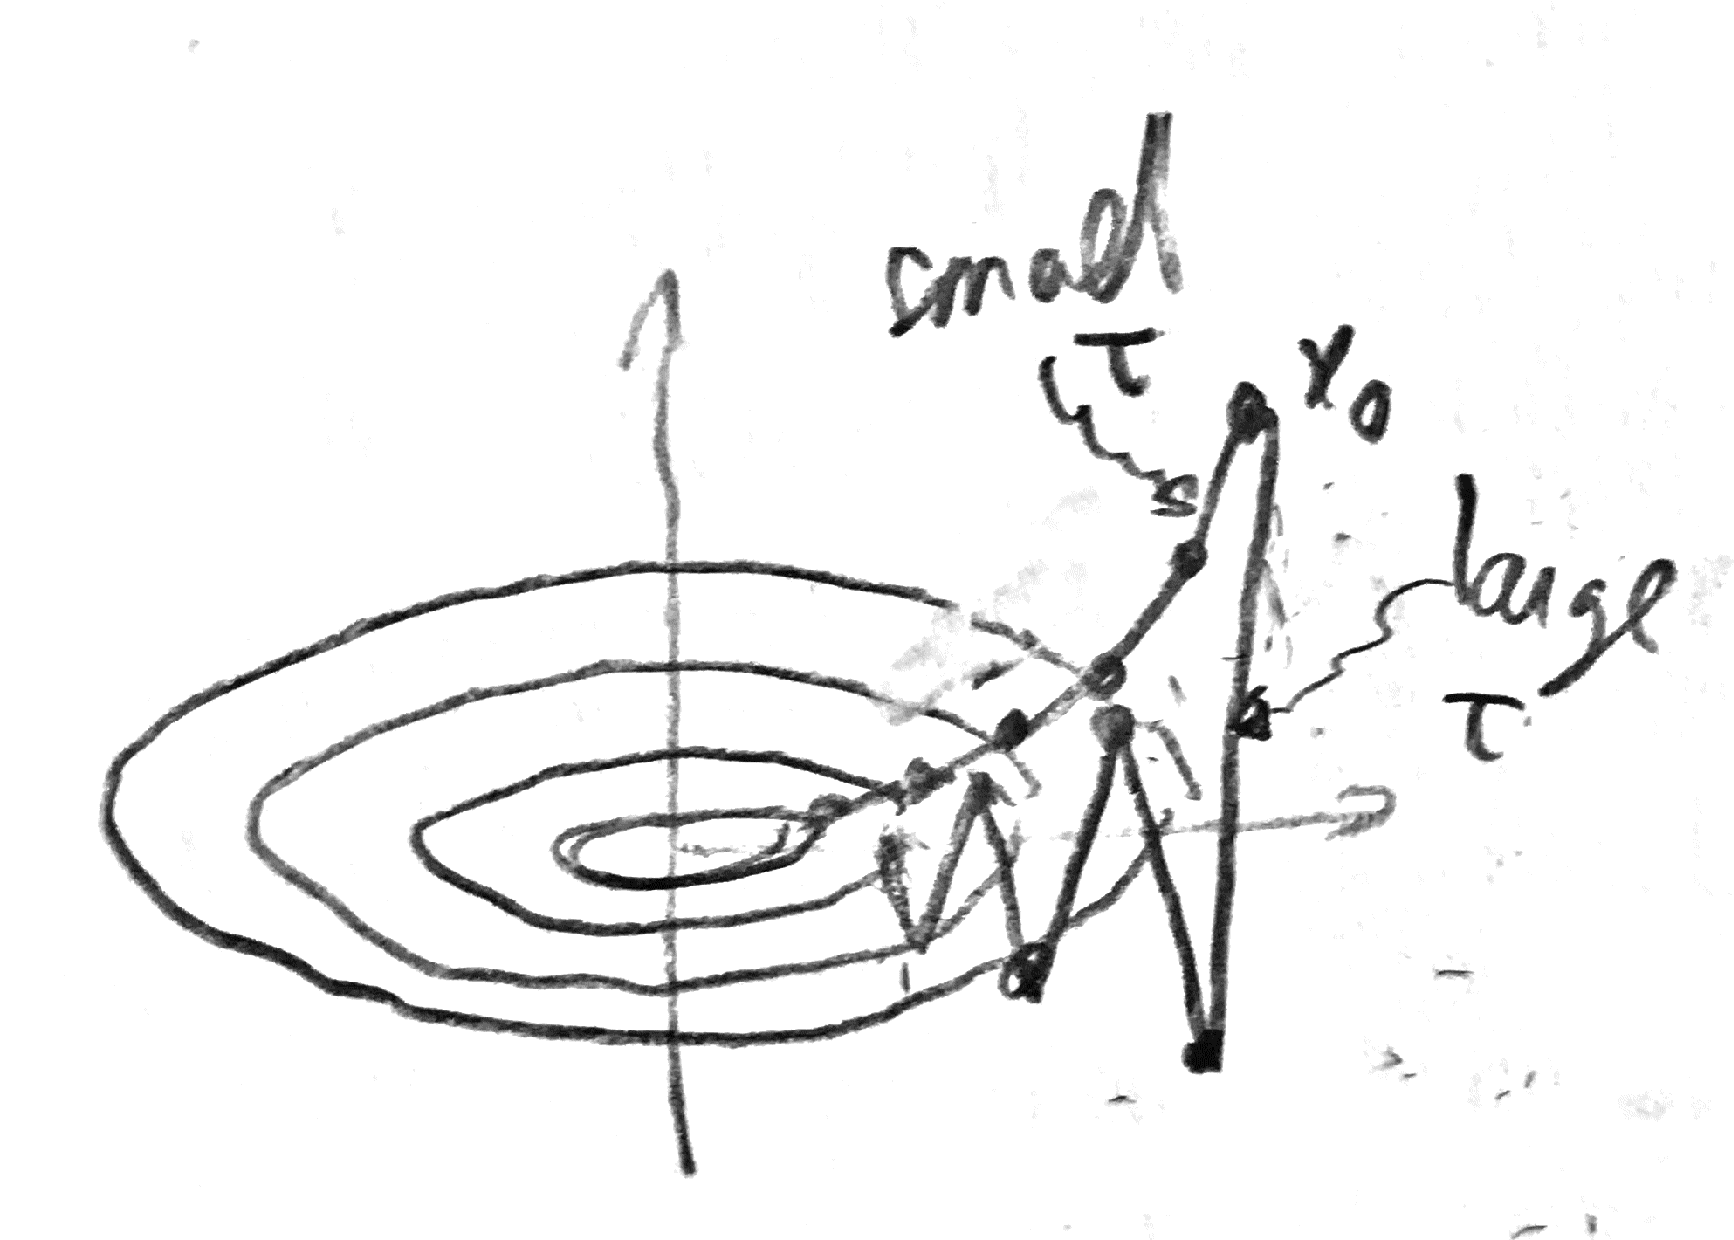
\includegraphics[width=.3\linewidth]{optim-smooth/grad-desc-1} \quad
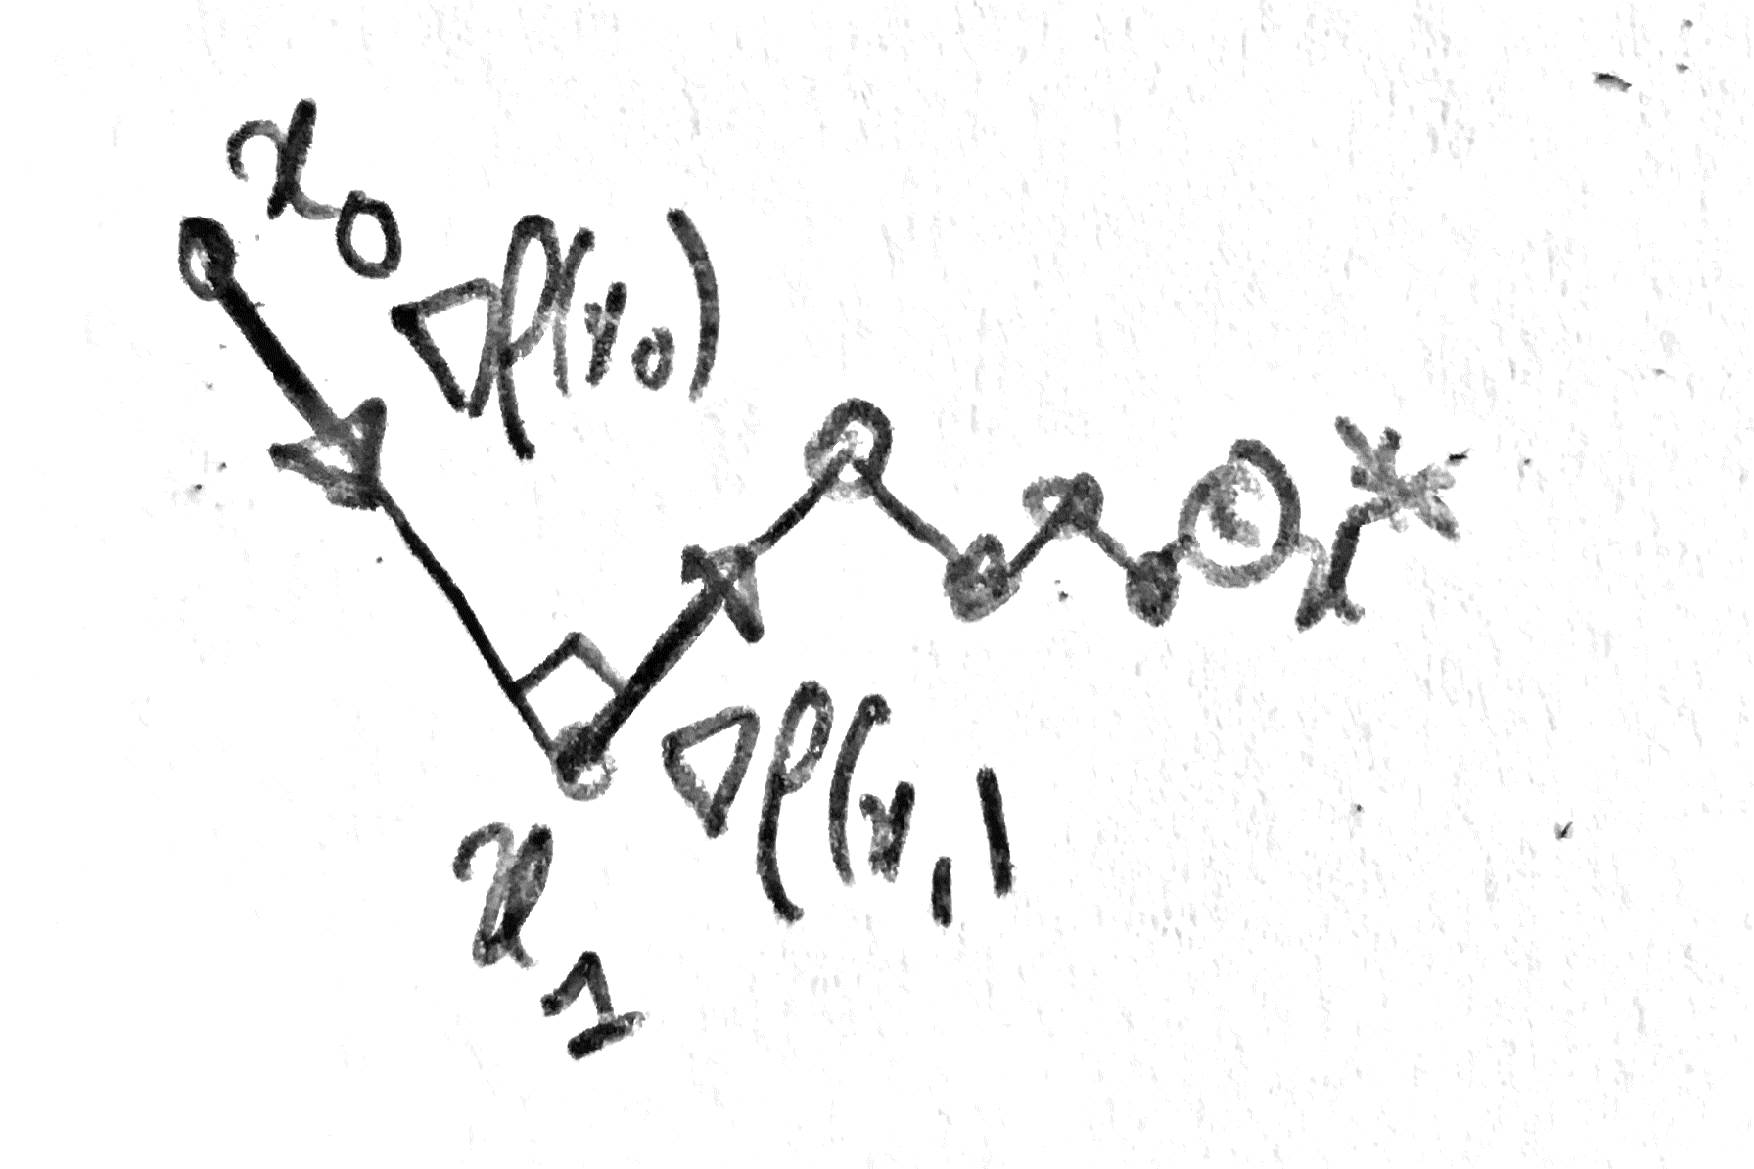
\includegraphics[width=.3\linewidth]{optim-smooth/grad-desc-2} 
\caption{\label{fig-gradesc}
Influence of $\tau$ on the gradient descent (left) and optimal step size choice (right).
}
\end{figure}


\begin{rem}[Greedy choice]
Although this is in general too costly to perform exactly, one can use a ``greedy'' choice, where the step size is optimal at each iteration, i.e. 
\eq{
	\tau_k \eqdef \uargmin{\tau} h(\tau) \eqdef f(x_k-\tau \nabla f(x_k)).
}
Here $h(\tau)$ is a function of a single variable. One can compute the derivative of $h$ as
\eq{
	h(\tau+\de) = f(x_k-\tau \nabla f(x_k) - \de \nabla f(x_k)) = f(x_k-\tau \nabla f(x_k))- \dotp{\nabla f(x_k-\tau \nabla f(x_k))}{ \nabla f(x_k)} + o(\de).
}
One note that at $\tau=\tau_k$, $\nabla f(x_k-\tau \nabla f(x_k))=\nabla f(x_{k+1})$ by definition of $x_{k+1}$ in~\eqref{eq-grad-desc}. 
%
Such an optimal $\tau=\tau_k$ is thus characterized by
\eq{
	h'(\tau_k) = - \dotp{\nabla f(x_k)}{\nabla f(x_{k+1})} = 0.
}
This means that for this greedy algorithm, two successive descent direction $\nabla f(x_k)$ and $\nabla f(x_{k+1})$ are orthogonal (see Fig.~\ref{fig-gradesc}).
\end{rem}




%%%%%%%%%%%%%%%%%%%%%%%%%%%%%%%%%%%%%%%%%%%%%%%%%%%%%%%%%%%%%%%%%%%%%%%%%%%%%%%%%%
%%%%%%%%%%%%%%%%%%%%%%%%%%%%%%%%%%%%%%%%%%%%%%%%%%%%%%%%%%%%%%%%%%%%%%%%%%%%%%%%%%
%%%%%%%%%%%%%%%%%%%%%%%%%%%%%%%%%%%%%%%%%%%%%%%%%%%%%%%%%%%%%%%%%%%%%%%%%%%%%%%%%%
\section{Convergence Analysis for the Quadratic Case}

%%%
\paragraph{Convergence analysis for the quadratic case.}

We first analyze this algorithm in the case of the quadratic loss, which can be written as
\eq{
	f(x) = \frac{1}{2}\norm{Ax-y}^2 = \frac{1}{2} \dotp{Cx}{x} - \dotp{x}{b} + \text{cst}
	\qwhereq
	\choice{
		C \eqdef A^\top A \in \RR^{p \times p}, \\
		b \eqdef A^\top y \in \RR^p. 
	}	
} 
We already saw that in~\eqref{eq-sol-leastsquare} if $\ker(A)=\{0\}$, which is equivalent to $C$ being invertible, then there exists a single global minimizer $x^\star = (A^\top A)^{-1} A^\top y = C^{-1} u$. 

Note that a function of the form $\frac{1}{2} \dotp{Cx}{x} - \dotp{x}{b}$ is convex if and only if the symmetric matrix $C$ is positive semi-definite, i.e. that all its eigenvalues are non-negative. \todo{detail this}

\begin{prop}\label{prop-graddesc-quad}
	For $f(x)=\dotp{Cx}{x}-\dotp{b}{x}$ ($C$ being symmetric semi-definite positive) with the eigen-values of $C$ upper-bounded by $L$ and lower-bounded by $\mu>0$, assuming there exists $(\tau_{\min},\tau_{\max})$ such that
	\eql{\label{eq-descent-step-cond}
		0 < \tau_{\min} \leq \tau_\ell \leq \tilde\tau_{\max} < \frac{2}{L}
	}
	then there exists $0 \leq \tilde\rho<1$ such that 
	\eql{\label{eq-global-linrate-grad}
		\norm{ x_k-x^\star } \leq \tilde\rho^\ell \norm{x_0-x^\star}.
	} 
	The best rate $\tilde\rho$ is obtained for 
	\eql{\label{eq-best-rate-local}
		\tau_\ell = \frac{2}{L+\mu}
		\qarrq
		\tilde\rho \eqdef \frac{L-\mu}{L+\mu} = 1 - \frac{2\epsilon}{1+\epsilon}
		\qwhereq
		\epsilon \eqdef \mu/L.
	} 
\end{prop}
\begin{proof}
	One iterate of gradient descent reads 
	\eq{
		x_{k+1}=x_k-\tau_\ell (C x_k-b).
	}	
	Since the solution $x^\star$ (which by the way is unique by strict convexity) satisfy the first order condition $C x^\star=b$, it gives
	\eq{
		x_{k+1}-x^\star =x_k-x^\star-\tau_\ell C(x_k-x^\star) = (\Id_p-\tau_\ell C)(x_k-x^\star).
	}	
	One thus has to study the contractance ratio of the linear map $\Id_p-\tau_\ell C$, i.e. its largest singular value, which reads
	\eq{
		h(\tau) \eqdef \norm{\Id_p-\tau C}_2 = \si_{\max}(\Id_p - \tau C)  = \max( |1-\tau_\ell \si_{\max}(C)|,|1-\tau \si_{\min}(C)| ).
	}
	For a quadratic function, one has $\si_{\min}(C) = \mu, \si_{\max}(C)=L$. Figure~\ref{fig-grad-desc-contract}, right, shows a display of $h(\tau)$. One has that for $0<\tau<2/L$, $h(\tau)<1$.
\end{proof}



\begin{figure}
\centering
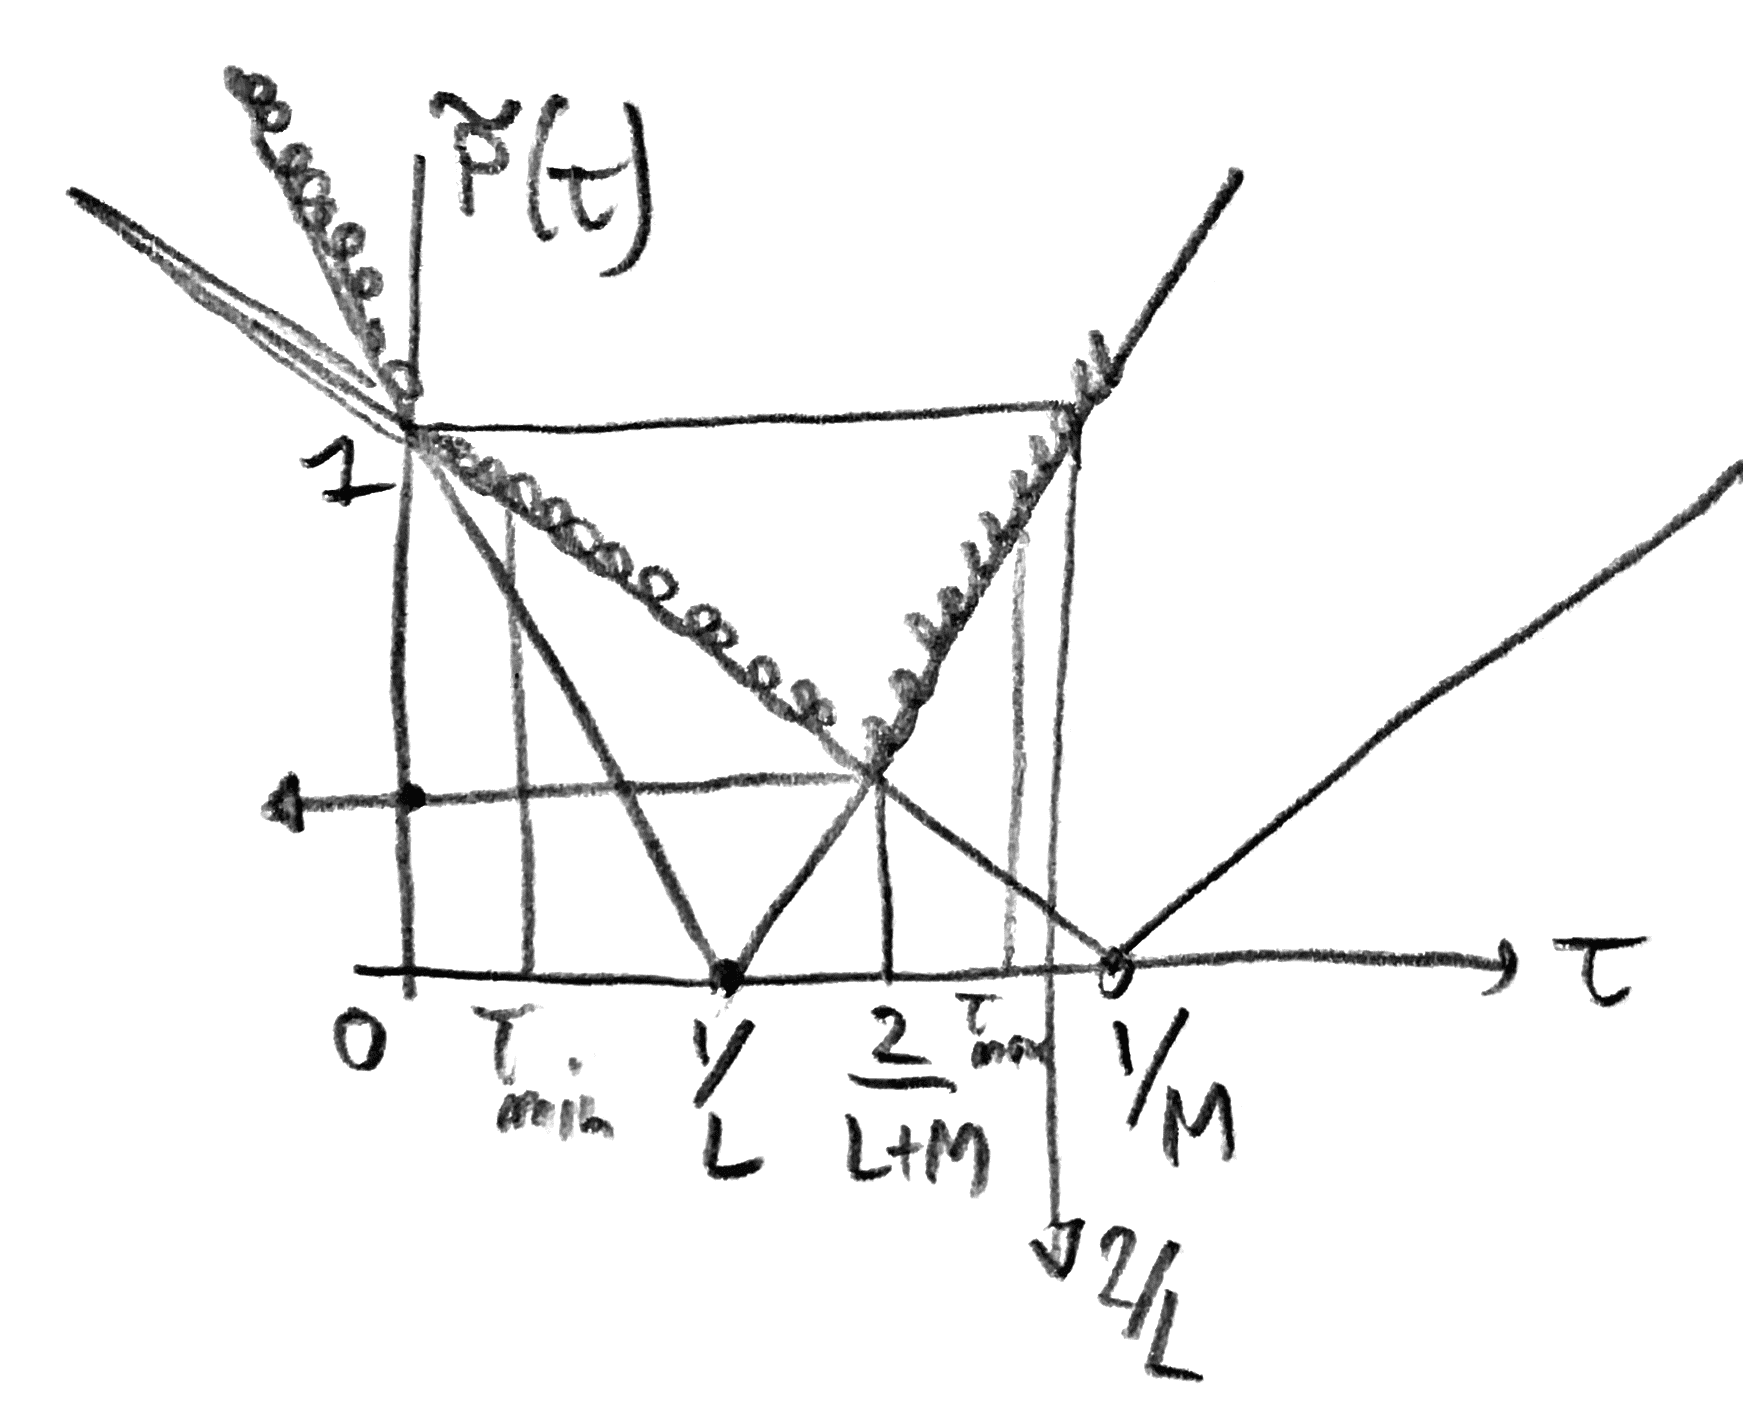
\includegraphics[width=.35\linewidth]{inverse-problems/grad-desc-linear}
\caption{\label{fig-grad-desc-contract}
Contraction constant $h(\tau)$ for a quadratic function (right). 
}
\end{figure}

Note that when the condition number $\epsilon \eqdef \mu/L \ll 1$
is small (which is the typical setup for ill-posed problems), then the contraction constant appearing in~\eqref{eq-best-rate-local} scales like 
\eql{\label{eq-rate-strong-quad}
	\tilde\rho \sim 1-2\epsilon.
}
%
The quantity $\epsilon$ in some sense reflects the inverse-conditioning of the problem. For quadratic function, it indeed corresponds exactly to the inverse of the condition number (which is the ratio of the largest to smallest singular value). The condition number is minimum and equal to $1$ for orthogonal matrices.

The error decay rate~\eqref{eq-global-linrate-grad}, although it is geometrical $O(\rho^\ell)$ is called a ``linear rate'' in the optimization literature. It is a ``global'' rate because it hold for all $\ell$ (and not only for large enough $\ell$).

If $\ker(A) \neq \{0\}$, then $C$ is not definite positive (some of its eigenvalues vanish), and the set of solution is infinite. 
%
One can however still show a linear rate, by showing that actually the iterations $x_k$ are orthogonal to $\ker(A)$ and redo the above proof replacing $\mu$ by the smaller non-zero eigenvalue of $C$. This analysis however leads to a very poor rate $\rho$ (very close to 1) because $\mu$ can be arbitrary close to 0. Furthermore, such a proof does not extends to non-quadratic functions. It is thus necessary to do a different theoretical analysis, which only shows a sublinear rate on the objective function $f$ itself rather than on the iterates $x_k$.  

\begin{prop}\label{prop-graddesc-quad}
	For $f(x)=\dotp{Cx}{x}-\dotp{b}{x}$, assuming the eigenvalue of $C$ are bounded by $L$, then if $0<\tau_\ell=\tau < 2/L$ is constant, then
	\eq{
		f(x_k)-f(x^\star) \leq \frac{\text{\upshape dist}(x_0,\argmin f)^2}{\tau 8 k}.
	}
	where 
	\eq{
		\text{\upshape dist}(x_0,\argmin f) \eqdef \umin{x^\star \in \argmin f} \norm{x_0-x^\star}.
	}
\end{prop}
\begin{proof}	
	We have $C x^\star=b$ for any minimizer $x^\star$
	and $x_{k+1}=x_k-\tau (C x_k-b)$ so that as before
	\eq{
		x_k-x^\star = (\Id_p-\tau C)^k(x_0-x^\star).
	}
	Now one has
	\eq{
		\frac{1}{2}\dotp{C(x_k-x^\star}{x_k-x^\star} = 
		\frac{1}{2}\dotp{Cx_k}{x_k} 
		- \dotp{Cx_k}{x^\star}
		+ \frac{1}{2} \dotp{Cx^\star}{x^\star}
	}
	and we have $\dotp{Cx_k}{x^\star} = \dotp{x_k}{Cx^\star} = \dotp{x_k}{b}$
	and also $\dotp{Cx^\star}{x^\star} = \dotp{x^\star}{x}$ so that
	\eq{
		\frac{1}{2}\dotp{C(x_k-x^\star}{x_k-x^\star} = 
		\frac{1}{2}\dotp{Cx_k}{x_k} - \dotp{x_k}{b}
		+ \frac{1}{2} \dotp{x^\star}{b}
		= f(x_k)-f(x^\star)
	}
	where we have used the fact that\todo{detail this}
	\eq{
		\frac{1}{2} \dotp{x^\star}{b} = -f(x^\star).	
	}
	This thus implies 
	\eq{
		f(x_k)-f(x^\star) = 
		\frac{1}{2}\dotp{(\Id_p-\tau C)^k C (\Id_p-\tau C)^k (x_0-x^\star)}{x_0-x^\star}
		\leq \frac{\si_{\max}(M_k)}{2} \umin{x^\star} \norm{x_0-x^\star}^2
	}
	where we have denoted
	\eq{
		M_k \eqdef (\Id_p-\tau C)^k C (\Id_p-\tau C)^k.
	}
	One has 
	\eq{
		\si_\ell(M_k) = \si_\ell(C) (1-\tau \si_\ell(C))^{2k}
			\leq \frac{1}{\tau 4 k}
	}
	since one can show that (setting $t = \tau \si_\ell(C) \leq 1$ because of the hypotheses)
	\eq{
		\foralls t \in [0,1], \quad
			(1-t)^{2k} t \leq \frac{1}{4k}.
	}
	Indeed, one has
	\begin{align*}
		(1-t)^{2k} t \leq (e^{-t})^{2k}t
		= \frac{1}{2k} (2kt) e^{-2k t}
		\leq \frac{1}{2k} \usup{u \geq 0} u e^{-u}
		= \frac{1}{2e k} \leq \frac{1}{4k}.
	\end{align*}
\end{proof}	
	


%%%%%%%%%%%%%%%%%%%%%%%%%%%%%%%%%%%%%%%%%%%%%%%%%%%%%%%%%%%%%%%%%%%%%%%%%%%%%%%%%%
%%%%%%%%%%%%%%%%%%%%%%%%%%%%%%%%%%%%%%%%%%%%%%%%%%%%%%%%%%%%%%%%%%%%%%%%%%%%%%%%%%
%%%%%%%%%%%%%%%%%%%%%%%%%%%%%%%%%%%%%%%%%%%%%%%%%%%%%%%%%%%%%%%%%%%%%%%%%%%%%%%%%%
\section{Convergence Analysis for the General Case}


\paragraph{Hessian.}

A differentiable function $f$ is said to be twice differentiable at $x$ if there exists a symmetric matrix (the hessian) $\partial^2 f(x) \in \RR^{p \times p}$ such that 
\eq{
	f(x+\epsilon) = f(x) + \dotp{\nabla f(x)}{\epsilon} + \frac{1}{2} \dotp{\partial^2 f(x) \epsilon}{\epsilon}
	+ o(\norm{\epsilon}^2).
}
This means that one can approximate $f$ near $x$ by a quadratic function. Roughly speaking, the theoretical analysis of the gradient descent for a generic function is obtained by applying this approximation and using the previous proof.

This Hessian can be obtained by performing an expansion (i.e. computing the differential) of the gradient since
\eq{
	\nabla f(x+\epsilon) = \nabla f(x) + [\partial^2 f(x)](\epsilon) + o(\norm{\epsilon})
}
where $[\partial^2 f(x)](\epsilon) \in \RR^p$ denotes the multiplication of the matrix $\partial^2 f(x)$ with the vector $\epsilon$. 

One can show that a twice differentiable function $f$ on $\RR^p$ is convex if and only if for all $x$ the symmetric matrix $\partial^2 f(x)$ is positive semi-definite, i.e. all its eigenvalues are non-negative. 
% 
Furthermore, if these eigenvalues are strictly positive then $f$ is strictly convex (but the converse is not true, for instance $x^4$ is strictly convex on $\RR$ but its second derivative vanishes at $x=0$). 

For instance, for a quadratic function $f(x)=\dotp{C x}{x} - \dotp{x}{u}$, one has $\nabla f(x) = Cx-u$ and thus $\partial^2 f(x) = C$ (which is thus constant).
%
For the classification function, one has 
\eq{
	\nabla f(x) = -A^\top \diag(y) \nabla L( -\diag(y) Ax). 
}
and thus
\begin{align*}
	\nabla f(x+\epsilon) &= -A^\top \diag(y) \nabla L( -\diag(y) Ax - -\diag(y) A\epsilon)  \\
		&= \nabla f(x)  -A^\top \diag(y) [\partial^2 L( -\diag(y) Ax)]( -\diag(y) A\epsilon) 
\end{align*}
Since $\nabla L(u) = (\ell'(u_i))$ one has $\partial^2 L(u)=\diag(\ell''(u_i))$. This means that 
\eq{
	\partial^2 f(x) = A^\top \diag(y) \times \diag( \ell''(-\diag(y) Ax) ) \times \diag(y) A.
}
One verifies that this matrix is symmetric and positive if $\ell$ is convex and thus $\ell''$ is positive. 



\paragraph{Smoothness and strong convexity.}

One also needs to quantify the smoothness of $f$. This is enforced by requiring that the gradient is $L$-Lipschitz, i.e.
\eql{\label{eq-lipsch-grad}\tag{$\Rr_L$}
	\foralls (x,x') \in (\RR^p)^2, \quad
	\norm{ \nabla f(x)-\nabla f(x') } \leq L \norm{x-x'}. 
}
In order to obtain fast convergence of the iterates themselve, it is needed that the function has enough ``curvature'' (i.e. is not too flat), which corresponds to imposing that $f$ is $\mu$-strongly convex
\eql{\label{eq-strong-conv}\tag{$\Ss_\mu$}
	\foralls (x,x'), \in (\RR^p)^2, \quad
	\dotp{\nabla f(x)-\nabla f(x')}{ x-x' } \geq \mu \norm{x-x'}^2. 
}
The following proposition express these conditions as constraints on the hessian for $\Cc^2$ functions.

\begin{prop}\label{prop-smooth-strong}
Conditions~\eqref{eq-lipsch-grad} and~\eqref{eq-strong-conv} imply
\eql{\label{eq-above-below-quad}
	\foralls (x,x'), \quad
	f(x') + \dotp{\nabla f(x)}{x'-x} + \frac{\mu}{2}\norm{x-x'}^2
	\leq
	f(x) 
	\leq 
	f(x') + \dotp{\nabla f(x')}{x'-x} + \frac{L}{2}\norm{x-x'}^2.
}
If $f$ is of class $\Cc^2$, conditions~\eqref{eq-lipsch-grad} and~\eqref{eq-strong-conv} are equivalent to
\eql{\label{eq-upper-lower-bound-hess}
	\foralls x, \quad \mu \Id_{p}  \preceq \partial^2 f(x) \preceq L \Id_{p}
}
where $\partial^2 f(x) \in \RR^{p \times p}$ is the Hessian of $f$, and 
where $\preceq$ is the natural order on symmetric matrices, i.e.
\eq{
	A \preceq B \quad\Longleftrightarrow\quad
	\foralls x \in \RR^p, \quad \dotp{A u}{u} \leq \dotp{B u}{u}.
}
\end{prop}

\begin{proof}
	We prove~\eqref{eq-above-below-quad}, using Taylor expansion with integral remain
	\eq{
		f(x') - f(x) = \int_0^1 \dotp{\nabla f(x_t)}{x'-x} \d t
		= \dotp{\nabla f(x)}{x'-x} + \int_0^1 \dotp{\nabla f(x_t)-\nabla f(x)}{x'-x} \d t		
	}
	where $x_t \eqdef f+t(x'-x)$.
	%
	Using Cauchy-Schwartz, and then the smoothness hypothesis~\eqref{eq-lipsch-grad}
	\eq{
		f(x') - f(x) \leq \dotp{\nabla f(x)}{x'-x} +  \int_0^1 L \norm{x_t-f} \norm{x'-x} \d t
		\leq \dotp{\nabla f(x)}{x'-x} +  L \norm{x'-x}^2 \int_0^1  t  \d t
	} 
	which is the desired upper-bound. Using directly~\eqref{eq-strong-conv} gives 
	\eq{
		f(x') - f(x) 
		= \dotp{\nabla f(x)}{x'-x} + \int_0^1 \dotp{\nabla f(x_t)-\nabla f(x)}{\frac{x_t-x}{t}} \d t	
		\geq \dotp{\nabla f(x)}{x'-x} + \mu \int_0^1 \frac{1}{t}\norm{x_t-x}^2  \d t
	}
	which gives the desired result since $\norm{x_t-x}^2 / t = t \norm{x'-x}^2$.
\end{proof}

The relation~\eqref{eq-above-below-quad} shows that a smooth (resp. strongly convex) functional is bellow a quadratic tangential majorant (resp. minorant). 

Condition~\eqref{eq-upper-lower-bound-hess} thus reads that the singular values of $\partial^2 f(x)$ should be contained in the interval $[\mu,L]$. The upper bound is also equivalent to $\norm{\partial^2 f(x)}_{\text{op}} \leq L$ where $\norm{\cdot}_{\text{op}}$ is the operator norm, i.e. the largest singular value. 
%
In the special case of a quadratic function $\Qq$ of the form~\eqref{eq-quad-func}, $\partial^2 f(x)=A$ is constant, so that $[\mu,L]$ can be chosen to be the range of the singular values of $A$.

%%%
\paragraph{Convergence analysis.}

We now give convergence theorem for a general convex function. On contrast to quadratic function, if one does not assumes strong convexity, one can only show a sub-linear rate on the function values (and no rate at all on the iterates themselves!). It is only when one assume strong convexity that linear rate is obtained. 
%
Note that in this case, the solution of the minimization problem is not necessarily unique.

\begin{thm}\label{thm-gradsec-non-strong-conv}
	If $f$ satisfy conditions~\eqref{eq-lipsch-grad}, assuming there exists $(\tau_{\min},\tau_{\max})$ such that
	\eql{\label{eq-descent-step-cond}
		0 < \tau_{\min} \leq \tau_\ell \leq \tau_{\max} < \frac{2}{L}, 
	}
	then $x_k$ converges to a solution $x^\star$ of~\eqref{eq-general-pbm} and
	there exists $C>0$ such that 
	\eql{\label{eq-sublin-rate-gd}
		f(x_k)-f(x^\star) \leq \frac{C}{\ell+1}.
	} 
	If furthermore $f$ is $\mu$-strongly convex, then there exists $0 \leq \rho < 1$ such that $\norm{x_k-x^\star} \leq \rho^\ell \norm{x_0-x^\star}$.
\end{thm}

\begin{proof}
	In the case where $f$ is not strongly convex, we only prove~\eqref{eq-sublin-rate-gd} since the proof that $x_k$ converges is more technical. Note indeed that if the minimizer $x^\star$ is non-unique, then it might be the case that the iterate $x_k$ ``cycle'' while approaching the set of minimizer, but actually convexity of $f$ prevents this kind of pathological behavior. 
	%
	For simplicity, we do the proof in the case $\tau_\ell = 1/L$, but it extends to the general case. 
	%
	The $L$-smoothness property imply~\eqref{eq-above-below-quad}, which reads
	\eq{
	f(x_{k+1}) 
		\leq 
		f(x_k) + \dotp{\nabla f(x_k)}{x_{k+1}-x_k} + \frac{L}{2}\norm{x_{k+1}-x_k}^2.
	}
	Using the fact that $x_{k+1}-x_k = -\frac{1}{L} \nabla f(x_k)$, one obtains
	\eql{\label{eq-proox-x'rad-nonstrong-1}
		f(x_{k+1}) 
		\leq 
		f(x_k) -  \frac{1}{L} \norm{\nabla f(x_k)}^2 + \frac{1}{2L} \norm{\nabla f(x_k)}^2
		\leq  f(x_k) -  \frac{1}{2L} \norm{\nabla f(x_k)}^2 
	}
	This shows that $(f(x_k))_\ell$ is a decaying sequence.
	%
	By convexity
	\eq{
		f(x_k) + \dotp{\nabla f(x_k)}{x^\star-x_k} \leq f(x^\star)
	}
	and plugging this in~\eqref{eq-proox-x'rad-nonstrong-1} shows
	\begin{align}
		f(x_{k+1})  &\leq   
		f(x^\star) - \dotp{\nabla f(x_k)}{x^\star-x_k} - \frac{1}{2L} \norm{\nabla f(x_k)}^2 \\
		&= f(x^\star) + \frac{L}{2}\pa{
			\norm{x_k-x^\star}^2 - \norm{x_k-x^\star-\frac{1}{L}\nabla f(x_k)}^2
		}\\
		&= f(x^\star) + \frac{L}{2}\pa{
			\norm{x_k-x^\star}^2 - \norm{x^\star-x_{k+1}}^2 }. \label{eq-conv-rate-proof-1}
	\end{align}
	Summing these inequalities for $\ell=0,\ldots,k$, one obtains
	\eq{
		\sum_{\ell=0}^k f(x_{k+1}) - (k+1) f(x^\star) \leq  \frac{L}{2}\pa{
			\norm{x_0-x^\star}^2 - \norm{x^{(k+1)}-x^\star}^2 }
	}
	and since $f(x_{k+1})$ is decaying $\sum_{\ell=0}^k f(x_{k+1}) \geq (k+1) f(x^{(k+1)})$, thus 
	\eq{
		f(x^{(k+1)}) - f(x^\star) \leq \frac{L \norm{x_0-x^\star}^2}{2(k+1)}
	}
	which gives~\eqref{eq-sublin-rate-gd} for $C \eqdef L \norm{x_0-x^\star}^2/2$.
	
	If we now assume $f$ is $\mu$-strongly convex, then, using $\nabla f(x^\star)=0$, one has $\frac{\mu}{2}\norm{x^\star-x}^2 \leq f(x)-f(x^\star)$ for all $x$. 
	%
	Re-manipulating~\eqref{eq-conv-rate-proof-1} gives
	\eq{
		\frac{\mu}{2}\norm{ x_{k+1} - x^\star}^2 \leq f(x_{k+1})-f(x^\star) \leq \frac{L}{2}\pa{
			\norm{x_k-x^\star}^2 - \norm{x^\star-x_{k+1}}^2 }, 
	}
	and hence
	\eql{\label{eq-rate-strong}
		\norm{ x_{k+1} - x^\star} \leq \sqrt{ \frac{L}{L+\mu} } \norm{ x_{k+1} - x^\star}, 
	}
	which is the desired result. 
\end{proof}

Note that in the low conditioning setting $\epsilon \ll 1$, one retrieve a dependency of the rate~\eqref{eq-rate-strong} similar to the one of quadratic functions~\eqref{eq-rate-strong-quad}, indeed 
\eq{
	\sqrt{ \frac{L}{L+\mu} } = (1+\epsilon)^{-\frac{1}{2}} \sim 1 - \frac{1}{2}\epsilon. 
}

%%%%%%%%%%%%%%%%%%%%%%%%%%%%%%%%%%%%%%%%%%%%%%%%%%%%%%%%%%%%%%%%%%%%%%%%%%%%%%%%%%%%%%%%%%%%%%%%%%%%%%%%%%%%%%%%%%%%%%%%%%%%%%%%%%
%%%%%%%%%%%%%%%%%%%%%%%%%%%%%%%%%%%%%%%%%%%%%%%%%%%%%%%%%%%%%%%%%%%%%%%%%%%%%%%%%%%%%%%%%%%%%%%%%%%%%%%%%%%%%%%%%%%%%%%%%%%%%%%%%%
%%%%%%%%%%%%%%%%%%%%%%%%%%%%%%%%%%%%%%%%%%%%%%%%%%%%%%%%%%%%%%%%%%%%%%%%%%%%%%%%%%%%%%%%%%%%%%%%%%%%%%%%%%%%%%%%%%%%%%%%%%%%%%%%%%
% !TEX root = ../FundationsDataScience.tex

%%%%%%%%%%%%%%%%%%%%%%%%%%%%%%%%%%%%%%%%%%%%%%%%%%%%%%%%%%%%%%%%%%%%%%%%
%%%%%%%%%%%%%%%%%%%%%%%%%%%%%%%%%%%%%%%%%%%%%%%%%%%%%%%%%%%%%%%%%%%%%%%%
%%%%%%%%%%%%%%%%%%%%%%%%%%%%%%%%%%%%%%%%%%%%%%%%%%%%%%%%%%%%%%%%%%%%%%%%
\section{Stochastic Optimization}
\label{sec-stochastic-optim}

We detail some important stochastic Gradient Descent methods, which enable to perform optimization in the setting where the number of samples $n$ is large and even infinite. 

% We set the classes indexes to be $\{-1,+1\}$, and remove empty features, normalize $X$. $n$ is the number of samples, $p$ is the dimensionality of the features,

%%%%%%%%%%%%%%%%%%%%%%%%%%%%%%%%%%%%%%%%%%%%%%%%%%%%%%%%
\subsection{Minimizing Sums and Expectation}

A large class of functionals in machine learning can be expressed as minimizing large sums of the form
\eql{\label{eq-min-sums}
	\umin{x \in \RR^p} f(x) \eqdef \frac{1}{n} \sum_{i=1}^n f_i(x)
}
or even expectations of the form
\eql{\label{eq-min-int}
	\umin{x \in \RR^p}  f(x) \eqdef \EE_{\zp \sim \pi}( f(x,\zp) ) = \int_{\Zz} f(x,z) \d\pi(z).
}
Problem~\eqref{eq-min-sums} can be seen as a special case of~\eqref{eq-min-int}, when using a discrete empirical uniform measure $\pi = \sum_{i=1}^n \de_i$ and setting $f(x,i)=f_i(x)$. One can also viewed~\eqref{eq-min-sums} as a discretized ``empirical'' version of~\eqref{eq-min-int} when drawing $(z_i)_i$ i.i.d. according to $\zp$ and defining $f_i(x)=f(x,z_i)$. In this setup,~\eqref{eq-min-sums} converges to~\eqref{eq-min-int} as $n \rightarrow +\infty$.

A typical example of such a class of problems is empirical risk minimization for linear model, where in these cases
\eql{\label{eq-stochastic-erm}
	f_i(x) = \ell(\dotp{a_i}{x},y_i)
	\qandq
	f(x,z) = \ell(\dotp{a}{x},y)
}
for $z=(a,y) \in \Zz = (\Aa=\RR^p) \times \Yy$ (typically $\Yy=\RR$ or $\Yy=\{-1,2\}$ for regression and classification), where $\ell$ is some loss function. 
%
We illustrate bellow the methods on binary logistic classification, where
\eql{\label{eq-stoch-logistic}
	\loss(s,y ) \eqdef \log( 1+\exp(-sy) ), 
}
see Section~\ref{sec-two-class-logit} for details. But this extends to arbitrary parametric models, and in particular deep neural networks as detailed in Section~\ref{sec-deepnet-discr}. 

While some algorithms (in particular batch gradient descent) are specific to finite sums~\eqref{eq-min-sums}, the stochastic methods we detail next work verbatim (with the same convergence guarantees) in the expectation case~\eqref{eq-min-int}. For the sake of simplicity, we however do the exposition for the finite sums case, which is sufficient in the vast majority of cases. But one should keep in mind that $n$ can be arbitrarily large, so it is not acceptable in this setting to use algorithms whose complexity per iteration depend on $n$.

The general idea underlying stochastic optimization methods is \textit{not} to have faster algorithms with respect to traditional optimization schemes such as those detailed in Chapter~\ref{chap-conv-duality}. In almost all cases, if $n$ is not too large so that one afford the price of doing a few non-stochastic iterations, then deterministic methods are faster. But if $n$ is so large that one cannot do even a single deterministic iteration, then stochastic methods allow one to have a fine grained scheme by breaking the cost of determinstic iterations in smaller chunks. Another advantage is that they are quite easy to parallelize. 


%%%%%%%%%%%%%%%%%%%%%%%%%%%%%%%%%%%%%%%%%%%%%%%%%%%%%%%%
\subsection{Batch Gradient Descent (BGD)}

The usual deterministic (batch) gradient descent (BGD) is studied in details in Section~\ref{eq-general-pbm}. Its iterations read
\eq{
	x_{k+1} = x_k - \tau_k \nabla f(x_k)
}
and the step size should be chosen as $0 < \tau_{\min} < \tau_k < \tau_{\max} \eqdef 2/L$ where $L$ is the Lipschitz constant of the gradient $\nabla f$. In particular, in this determinstic setting, this step size should not go to zero and this ensures quite fast convergence (even linear rates if $f$ is strongly convex).

The computation of the gradient in our setting reads
\eql{\label{eq-full-grad}
	\nabla f(x) = \frac{1}{n} \sum_{i=1}^n \nabla f_i(x)
}
so it typically has complexity $O(np)$ if computing $\nabla f_i$ has linear complexity in $p$.

In the ERM setting~\eqref{eq-stochastic-erm}, the gradient reads \todo{detail here}
\eql{\label{eq-grad-formula}
	\nabla f_i(x) =  \ell'( \dotp{a_i}{x},y_i ) a_i,
}
% where $\partial f(a,x) \in \RR^{q \times p}$ is the Jacobian of the mapping $x \in \RR^p \mapsto f(a,x) \in \RR^q$, while
where $\ell( y,y' ) \in \RR$ is the derivative with respect to the first variable, i.e. the gradient of the map $y \in \RR \mapsto \loss(y,y') \in \RR$.
%
For the logistic loss, it is simply 
\eq{
	\loss'(s,y) = -s \frac{e^{-sy}}{ 1+e^{-sy} }.
}

\begin{figure}
\centering
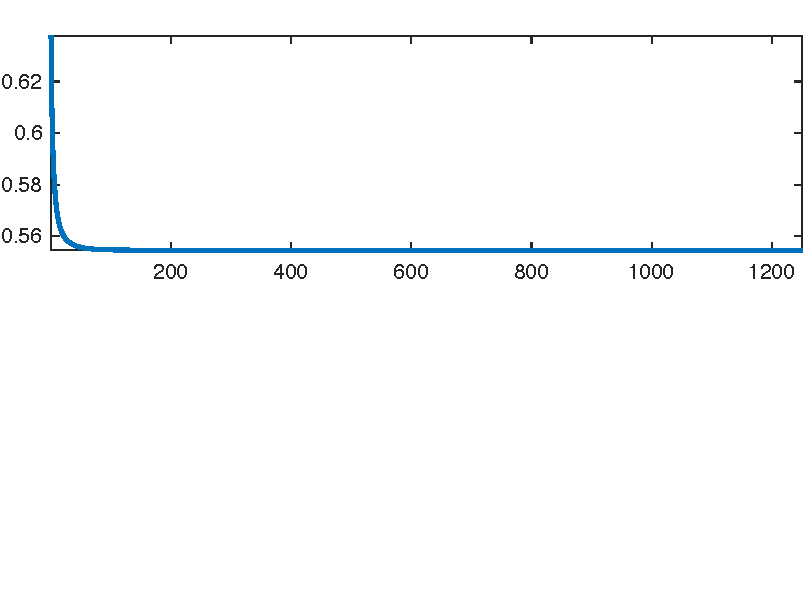
\includegraphics[width=.6\linewidth]{ml/sgd/error-bgd-1} \\
$f(x_k)$ \\
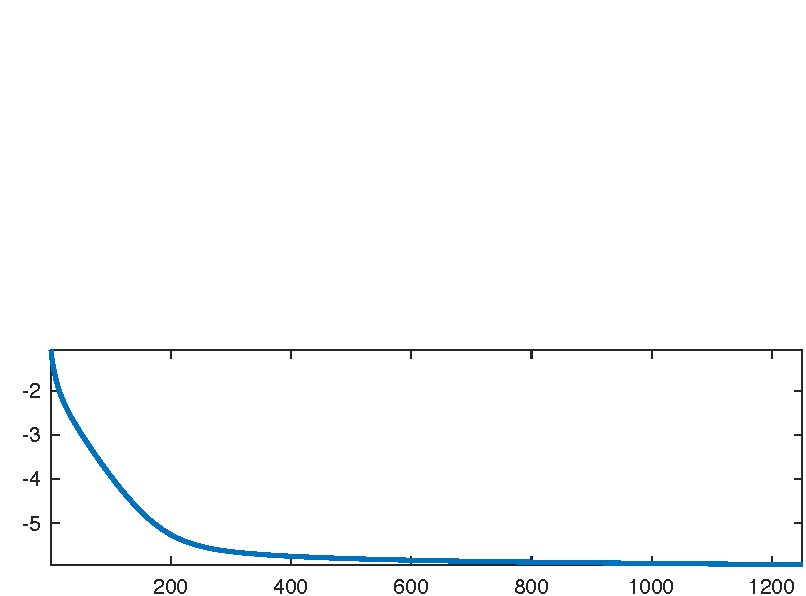
\includegraphics[width=.6\linewidth]{ml/sgd/error-bgd-2} \\
$\log_{10}(f(x_k)-f(x^\star))$ 
\caption{\label{fig-bgd}
Evolution of the error of the BGD for logistic classification.
}
\end{figure}



%%%%%%%%%%%%%%%%%%%%%%%%%%%%%%%%%%%%%%%%%%%%%%%%%%%%%%%%
\subsection{Stochastic Gradient Descent (SGD)}

\wrapf{ml/sgd/unbiased-grad}{Unbiased gradient estimate}
For very large $n$, computing the full gradient $\nabla f$ as in~\eqref{eq-full-grad} is prohibitive.  
%
The idea of SGD is to trade this exact full gradient by an inexact proxy using a single functional $f_{i}$ where $i$ is drawn uniformly at random. The main idea that makes this work is that this sampling scheme provides an unbiased estimate of the gradient, in the sense that
\eql{\label{eq-unbiased-grad}
	\EE_{\ip}{ \nabla f_{\ip}(x) } = \nabla f(x)
}
where $\ip$ is a random variable distributed uniformly in $\{1,\ldots,n\}$.

\wrapf{ml/sgd/sgd-schematic}{Schematic view of SGD iterates}
Starting from some $x^{(0)}$,the iterations of stochastic gradient descent (SGD) read
\eq{
	x_{k+1} = x_k - \tau_k \nabla f_{i(k)}(x_k)
}
where, for each iteration index $k$, $i(k)$
is drawn uniformly at random in $\{1,\ldots,n\}$. 
%
It is important that the iterates $x_{k+1}$ are thus random vectors, and the theoretical analysis of the method thus studies wether this sequence of random vectors converges (in expectation or in probability for instance) toward a deterministic vector (minimizing $f$), and at which speed. 

Note that each step of a batch gradient descent has complexity $O(np)$,
while a step of SGD only has complexity $O(p)$. SGD is thus
advantageous when $n$ is very large, and one cannot afford to do
several passes through the data. In some situation, SGD can provide
accurate results even with $k \ll n$, exploiting redundancy between
the samples.

A crucial question is the choice of step size schedule $\tau_k$. It
must tends to 0 in order to cancel the noise induced on the gradient by
the stochastic sampling. But it should not go too fast to zero in order
for the method to keep converging. 


A typical schedule that ensures both properties is to have asymptotically $\tau_k \sim k^{-1}$ for
$k\rightarrow +\infty$. We thus propose to use 
\eql{\label{eq-stepsize-sgd}
	\tau_k \eqdef \frac{\tau_0}{1 + k/k_0}
}
where $k_0$ indicates roughly the number of iterations serving as a
``warmup'' phase.

Figure~\ref{fig-sgd-traject} shows a simple 1-D example to minimize $f_1(x)+f_2(x)$ for $x \in \RR$ and $f_1(x)=(x-1)^2$ and $f_2(x)=(x+1)^2$. One can see how the density of the distribution of $x_k$ progressively clusters around the minimizer $x^\star=0$. Here the distribution of $x^{(0)}$ is uniform on $[-1/2,1/2]$.

\begin{figure}
\centering
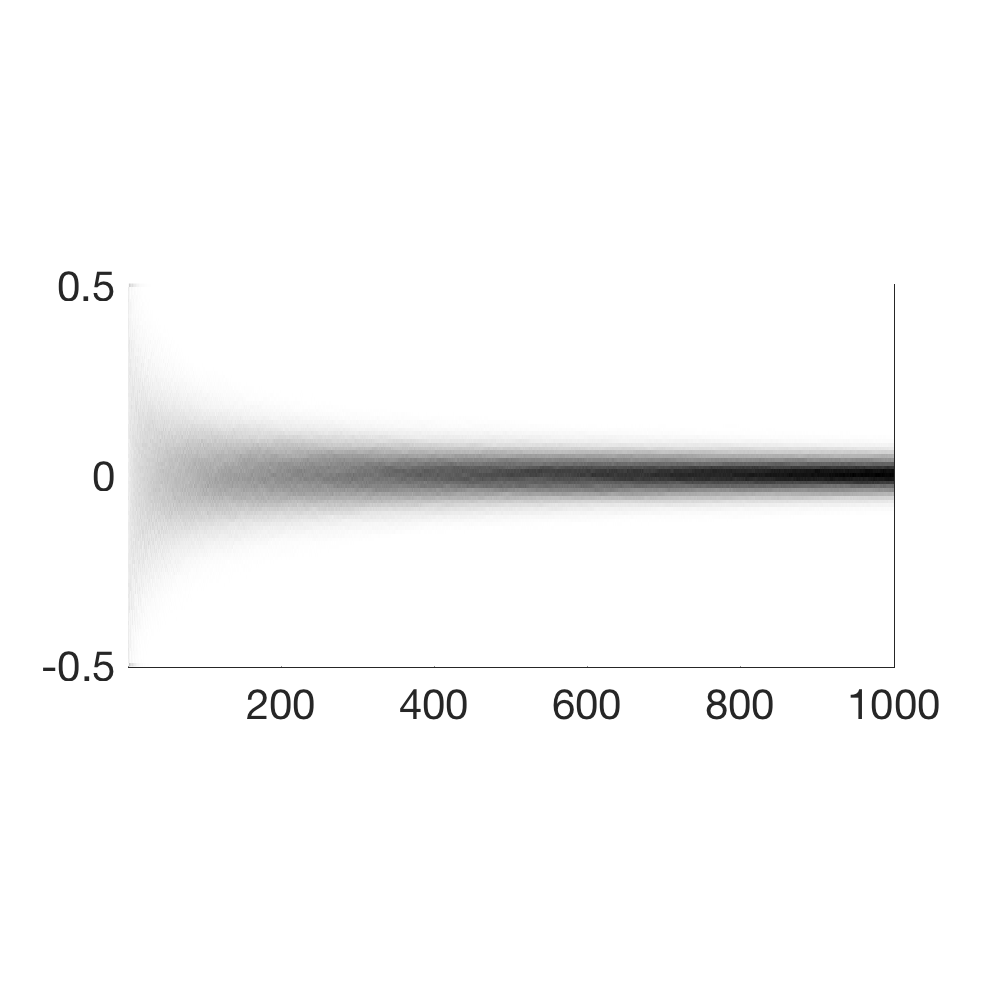
\includegraphics[width=.49\linewidth]{ml/sgd/sgd-histo} 
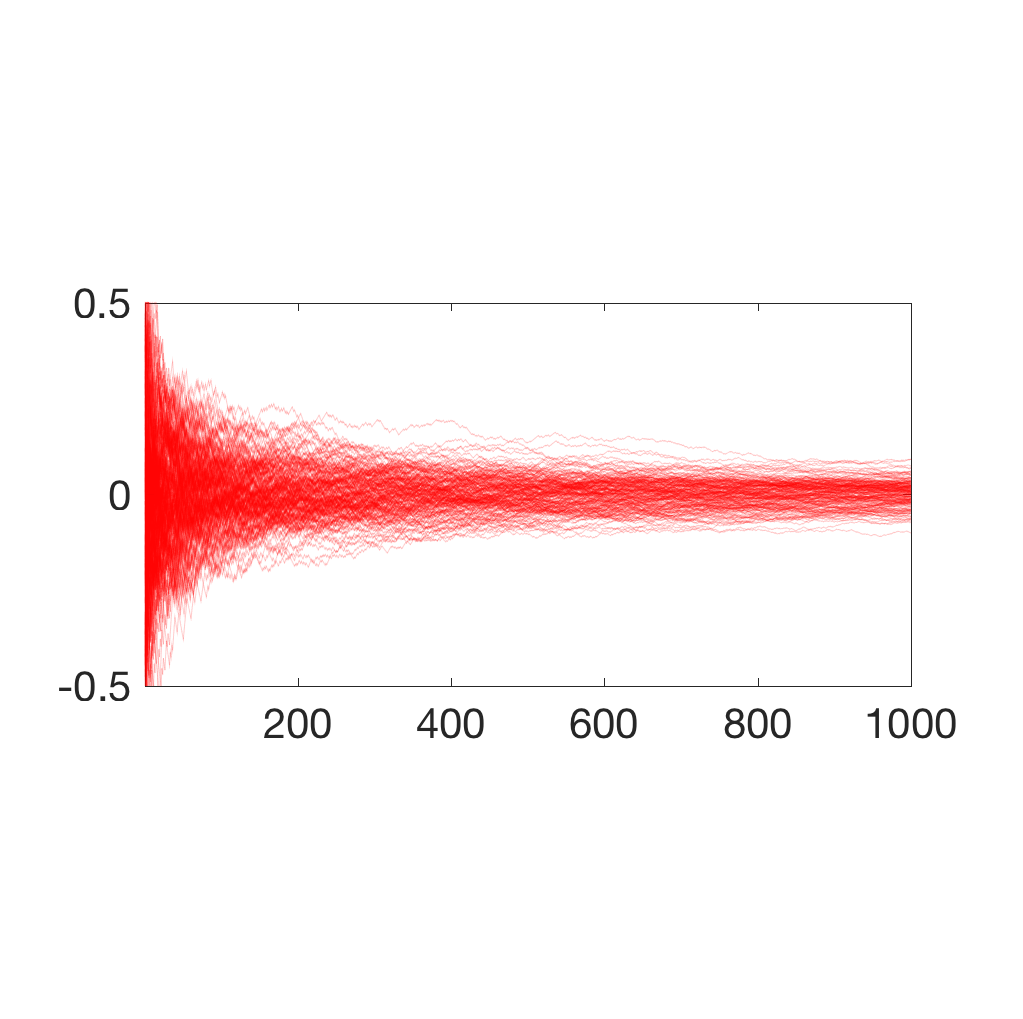
\includegraphics[width=.49\linewidth]{ml/sgd/sgd-trajectory}
\caption{\label{fig-sgd-traject}
Display of a large number of trajectories $k \mapsto x_k \in \RR$ generated by several runs of SGD. On the top row, each curve is a trajectory, and the bottom row displays the corresponding density.
}
\end{figure}


The following theorem shows the convergence in expectration with a $1/\sqrt{k}$ rate on the objective.

\begin{thm}\label{thm-conv-sgd}
We assume $f$ is $\mu$-strongly convex as defined in~\eqref{eq-strong-conv} (i.e. $\Id_{N \times N}  \preceq \partial^2  f(x)$ if $f$ is $\Cc^2$), and is such that $\norm{\nabla f_i(x)}^2 \leq C^2$. 
For the step size choice $\tau_k = \frac{1}{\mu (k+1)}$, one has
\eql{\label{eq-rate-sgd}
	\EE( \norm{x_k-x^\star}^2 ) \leq \frac{ R }{k+1}
	\qwhereq
	 R = \max( \norm{x^{(0)} - x^\star}, C^2/\mu^2 ), 
}
where $\EE$ indicates an expectation with respect to the i.i.d.
sampling performed at each iteration.
\end{thm}

\begin{proof}
	By strong convexity, one has
	\begin{align*}
		f(x^\star) - f(x_k) &\geq \dotp{ \nabla f(x_k) }{ x^\star-x_k } + \frac{\mu}{2}\norm{x_k-x^\star}^2 \\
		f(x_k) - f(x^\star) &\geq \dotp{ \nabla f(x^\star) }{ x_k - x^\star } + \frac{\mu}{2}\norm{x_k-x^\star}^2.
	\end{align*}
	Summing these two inequalities and using $\nabla f(x^\star)=0$ leads to
	\eql{\label{eq-sgd-proof-1}
		\dotp{ \nabla f(x_k) - \nabla f(x^\star) }{ x_k - x^\star }
		=
		\dotp{ \nabla f(x_k)  }{ x_k - x^\star }
		\geq \mu \norm{x_k-x^\star}^2.
	}
	Considering only the expectation with respect to the ransom sample of $i(k) \sim \ip_k$, one has
	\begin{align*}
		\EE_{\ip_k}( \norm{x_{k+1}-x^\star}^2 )
		&= 
		\EE_{\ip_k}( \norm{x_k - \tau_k \nabla f_{\ip_k}(x_k) -x^\star}^2 ) \\
		&= 
		\norm{x_k - x^\star}^2 + 2\tau_k \dotp{ \EE_{\ip_k}(\nabla f_{\ip_k}(x_k)) }{ x^\star - x_k  } + 
			\tau_k^2  \EE_{\ip_k}( \norm{\nabla f_{\ip_k}(x_k)}^2 ) \\
		&\leq
		\norm{x_k - x^\star}^2 + 2\tau_k \dotp{ \nabla f(x_k)) }{ x^\star - x_k  } + \tau_k^2 C^2 \\
	\end{align*}
	where we used the fact~\eqref{eq-unbiased-grad} that the gradient is unbiased. 
	%
	Taking now the full expectation with respect to all the other previous iterates, and using~\eqref{eq-sgd-proof-1} one obtains
	\eql{\label{eq-sgd-proof-2}
		\EE( \norm{x_{k+1}-x^\star}^2 ) \leq \EE( \norm{x_k - x^\star}^2 ) - 2 \mu \tau_k \EE( \norm{x_k - x^\star}^2 ) + \tau_k^2 C^2
		= (1-2 \mu \tau_k)  \EE( \norm{x_k - x^\star}^2 ) + \tau_k^2 C^2.
	}
	We show by recursion that the bound~\eqref{eq-rate-sgd} holds. We denote $\epsilon_k \eqdef \EE( \norm{x_k-x^\star}^2 )$.
	%
	Indeed, for $k=0$, this it is true that 
	\eq{
		\epsilon_0 \leq \frac{ \max( \norm{x^{(0)} - x^\star}, C^2/\mu^2 ) }{1} = \frac{R}{1}.
	}
	We now assume that $\epsilon_k \leq \frac{R}{k+1}$. Using~\eqref{eq-sgd-proof-2} in the case of $\tau_k = \frac{1}{\mu (k+1)}$, one has, denoting $m=k+1$
	\begin{align*}
		\epsilon_{k+1} &\leq (1-2 \mu \tau_k) \epsilon_k + \tau_k^2 C^2 = 
			\pa{1-\frac{2}{m}} \epsilon_k + \frac{C^2}{(\mu m)^2}  \\  
			&\leq
			\pa{1-\frac{2}{m}} \frac{R}{m} + \frac{R}{m^2}  = 
			\pa{ \frac{1}{m}-\frac{1}{m^2} } R
			= 
			\frac{m-1}{m^2} R
			= 
			\frac{m^2-1}{m^2}\frac{1}{m+1} R
			\leq
			\frac{R}{m+1}
	\end{align*}
\end{proof}

A weakness of SGD (as well as the SGA scheme studied next) is that it only weakly benefit from strong convexity of $f$. This is in sharp contrast with BGD, which enjoy a fast linear rate for strongly convex functionals, see Theorem~\ref{thm-gradsec-non-strong-conv}.

Figure~\ref{fig-sgd} displays the evolution of the energy $f(x_k)$. 
It overlays on top (black dashed curve) the convergence of the batch gradient descent, with a careful scaling of the 
number of iteration to account for the fact that the complexity of a batch iteration is $n$ times larger. 


\begin{figure}
\centering
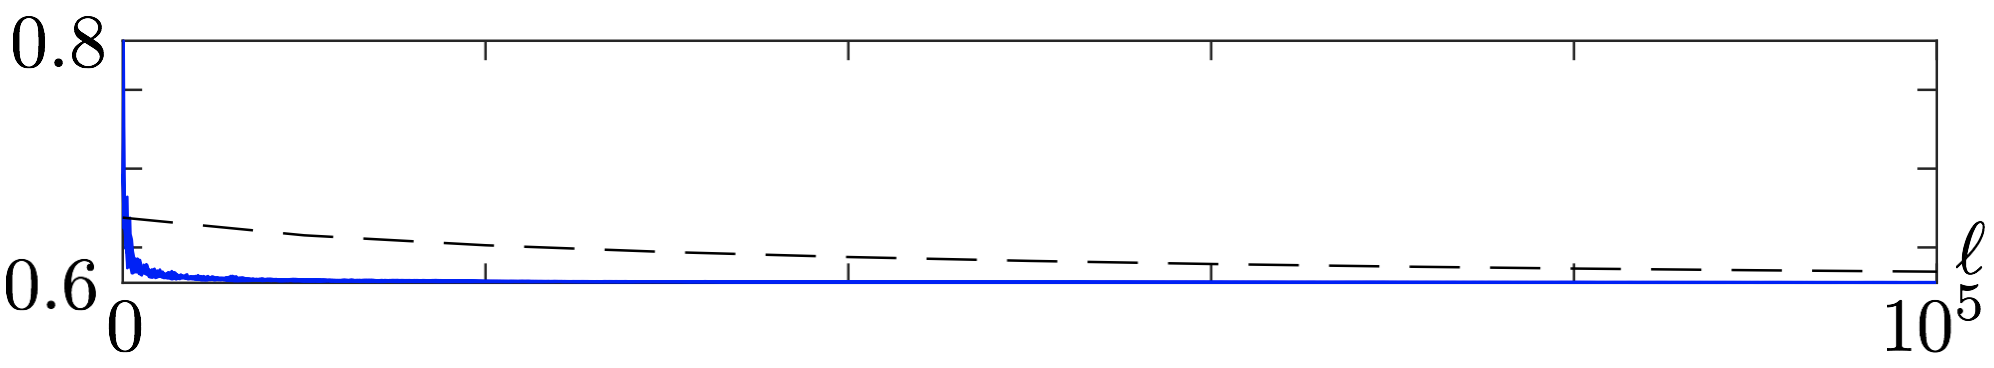
\includegraphics[width=.6\linewidth]{ml/sgd/error-sgd-1} \\
$f(x_k)$ \\
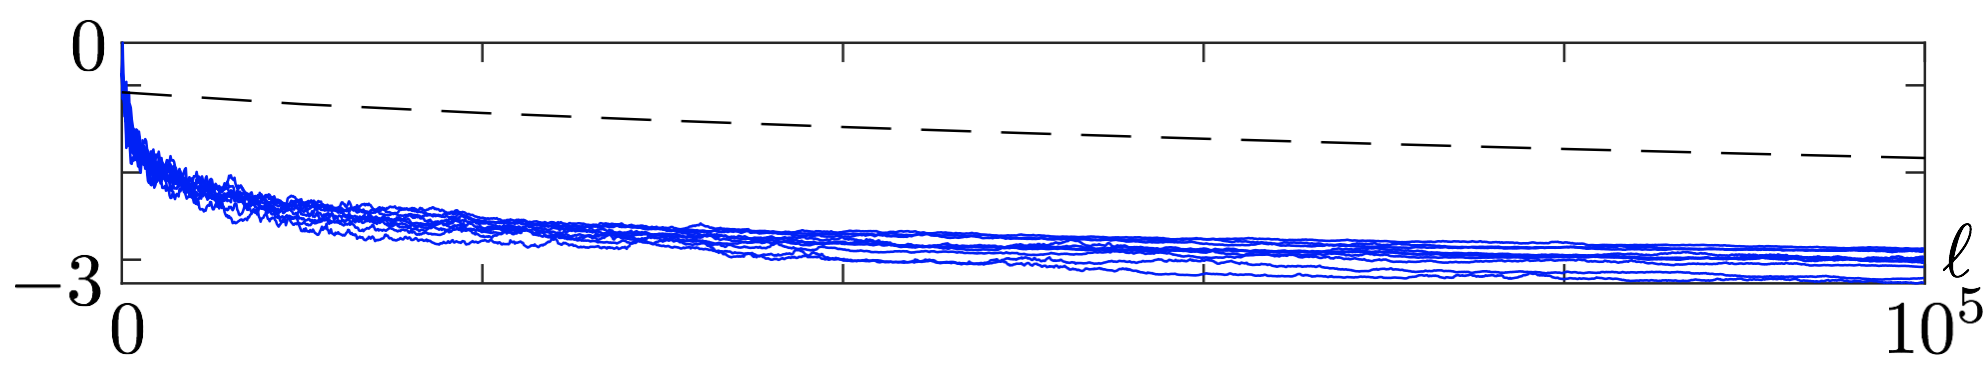
\includegraphics[width=.6\linewidth]{ml/sgd/error-sgd-2} \\
$\log_{10}(f(x_k)-f(x^\star))$ 
\caption{\label{fig-sgd}
Evolution of the error of the SGD for logistic classification (dashed line shows BGD).
}
\end{figure}




%%%%%%%%%%%%%%%%%%%%%%%%%%%%%%%%%%%%%%%%%%%%%%%%%%%%%%%%
\subsection{Stochastic Gradient Descent with Averaging (SGA)}
\label{sec-sga}

Stochastic gradient descent is slow because of the fast decay of
$\tau_k$ toward zero.
%
To improve somehow the convergence speed, it is possible to average the past
iterate, i.e. run a ``classical" SGD on auxiliary variables $( \tilde x_k)_k$
\eq{
	 \iit{\tilde x} = \tilde x_k - \tau_k \nabla f_{i(k)}(\tilde x_k)
}
and output as estimated weight vector the Cesaro average
\eq{
	x_k \eqdef \frac{1}{k} \sum_{\ell=1}^k \tilde x_{\ell}.
}
This defines the Stochastic Gradient Descent with Averaging (SGA)
algorithm.

Note that it is possible to avoid explicitly storing all the iterates by simply
updating a running average as follow
\eq{
	x_{k+1} = \frac{1}{k} \tilde x_k +  \frac{k-1}{k} x_k. 
}


In this case, a typical choice of decay is rather of the form 
\eq{
	\tau_k \eqdef \frac{\tau_0}{1 + \sqrt{k/k_0}}.
}
Notice that the step size now goes much slower to 0, at rate $k^{-1/2}$.


Typically, because the averaging stabilizes the iterates, the choice of
$(k_0,\tau_0)$ is less important than for SGD. 

% <https://arxiv.org/pdf/1303.6149.pdf 

Bach proves that for logistic classification, 
it leads to a faster convergence (the constant involved are
smaller) than SGD, since 
on contrast to SGD, SGA is adaptive to the local strong convexity of $E$.



%%%%%%%%%%%%%%%%%%%%%%%%%%%%%%%%%%%%%%%%%%%%%%%%%%%%%%%%
\subsection{Stochastic Averaged Gradient Descent (SAG)}

% https://arxiv.org/pdf/1309.2388
For problem size $n$ where the dataset (of size $n \times p$) can
fully fit into memory, it is possible to further improve the SGA method
by bookkeeping the previous gradients. This gives rise to the 
Stochastic Averaged Gradient Descent (SAG) algorithm.

We store all the previously computed gradients in $(G^i)_{i=1}^n$,
which necessitates $O(n \times p)$ memory. 
The iterates are defined by using a proxy $g$ for the batch gradient,
which is progressively enhanced during the iterates.

The algorithm reads
\eq{
	h \leftarrow \nabla f_{i(k)}(\tilde x_k),
}
\eq{
	g  \leftarrow g - G^{i(k)} + h,  
}
\eq{
	G^{i(k)} \leftarrow h, 
}
\eq{
	x_{k+1} = x_k - \tau g. 
}
Note that in contrast to SGD and SGA, this method uses a fixed step
size $\tau$. Similarly to the BGD, in order to ensure convergence, 
the step size $\tau$ should be of the order of $1/L$
where $L$ is the Lipschitz constant of $f$.

This algorithm improves over SGA and SGD
since it has a convergence rate of $O(1/k)$ as does BGD. 
Furthermore, in the presence of strong convexity (for instance when $X$ is
injective for logistic classification), it has a linear convergence rate, 
i.e. 
 \eq{
	\EE( f(x_k) ) - f(x^\star) = O\pa{ \rho^k },
}
for some $0 < \rho < 1$. 

Note that this improvement over SGD and SGA is made possible only because
SAG explicitly uses the fact that $n$ is finite (while SGD and SGA can
be extended to infinite $n$ and more general minimization of
expectations~\eqref{eq-min-int}).

Figure~\ref{fig-bgd} shows a comparison of SGD, SGA and SAG.

\begin{figure}
\centering
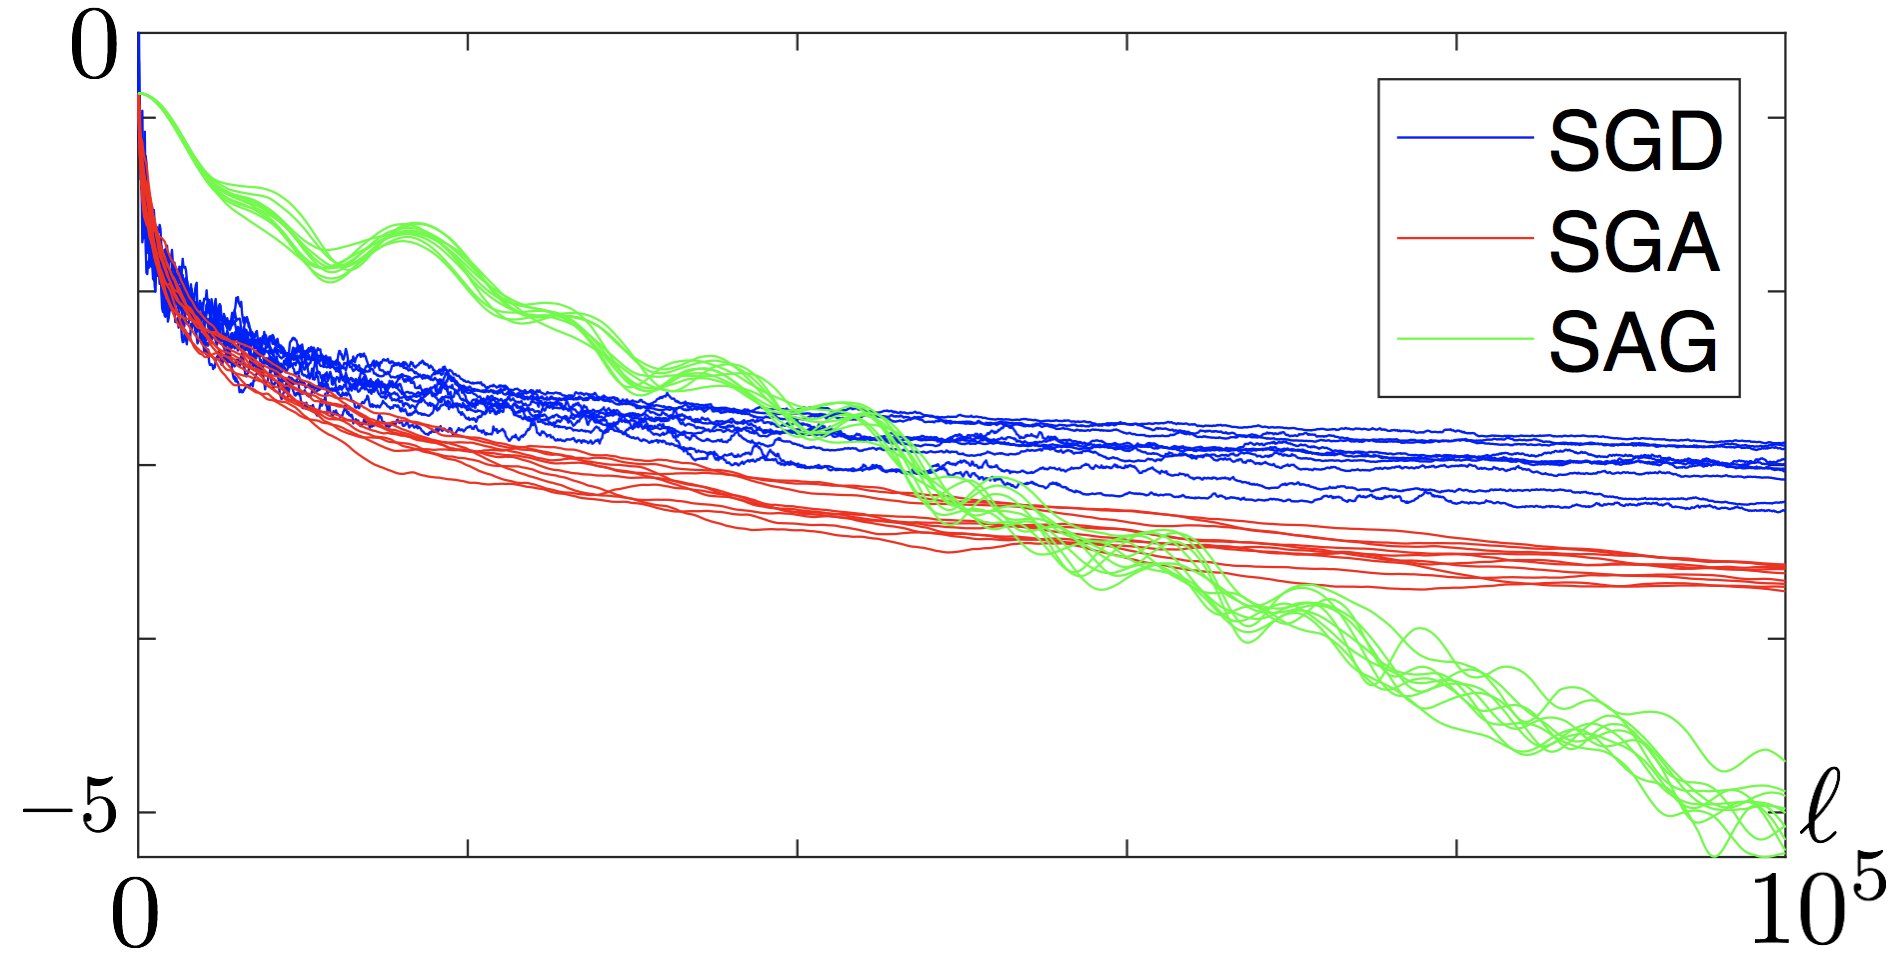
\includegraphics[width=.6\linewidth]{ml/sgd/sg-comparison}
\caption{\label{fig-bgd}
Evolution of $\log_{10}(f(x_k)-f(x^\star))$ for SGD, SGA and SAG.
}
\end{figure}







%%%%%%%%%%%%%%%%%%%%%%%%%%%%%%%%%%%%%%%%%%%%%%%%%%%%%%%%%%%%%%%%%%%%%%%%%%%%%%%%%%%%%%%%%%%%%%%%%%%%%%%%%%%%%%%%%%%%%%%%%%%%%%%%%%
%%%%%%%%%%%%%%%%%%%%%%%%%%%%%%%%%%%%%%%%%%%%%%%%%%%%%%%%%%%%%%%%%%%%%%%%%%%%%%%%%%%%%%%%%%%%%%%%%%%%%%%%%%%%%%%%%%%%%%%%%%%%%%%%%%
%%%%%%%%%%%%%%%%%%%%%%%%%%%%%%%%%%%%%%%%%%%%%%%%%%%%%%%%%%%%%%%%%%%%%%%%%%%%%%%%%%%%%%%%%%%%%%%%%%%%%%%%%%%%%%%%%%%%%%%%%%%%%%%%%%
% !TEX root = ../FundationsDataScience.tex

%%% SECTION PART OF optim-smooth.tex

%%%%%%%%%%%%%%%%%%%%%%%%%%%%%%%%%%%%%%%%%%%%%%%%%%%%%%%%%%%%%%%%%%%%%%%%
%%%%%%%%%%%%%%%%%%%%%%%%%%%%%%%%%%%%%%%%%%%%%%%%%%%%%%%%%%%%%%%%%%%%%%%%
%%%%%%%%%%%%%%%%%%%%%%%%%%%%%%%%%%%%%%%%%%%%%%%%%%%%%%%%%%%%%%%%%%%%%%%%
\section{Automatic Differentiation}

The main computational bottleneck of these gradient descent methods (batch or stochastic) is the evaluation of the elementary gradients $\nabla \Ee_i$. The gradient formula~\eqref{eq-grad-formula} shows that it requires to remap the gradient of the loss $\nabla \loss( f(x_i,\be),y_i )$ through the adjoint of the Jacobian $\partial f(x_i,\be)$. 
%
The general idea is that for complicated model this computation should be broken in simpler sub-computation, which ultimately should corresponds to elementary operators (binary operators such as + or * and unary operators such as exp, log, etc.) for which the differential are trivial to compute.

%%%%%%%%%%%%%%%%%%%%%%%%%%%%%%%%%%%%%%%%%%%%%%%%%%%%%%%%%%%%%%%%%%%%%%%%
\subsection{Reverse Differentiation on a Feedforward Graph}
\label{sec-reversemode-simple}

To give a concrete examples which is actually found in many practical situation (and in particular for simple deep architectures, as detailed in Section~\ref{sec-deep-structure}), if the functional to be differentiated has the form 
\eql{\label{eq-simple-lin-dag}
	\Ee(\be) = \Ll \circ \Ff_{L-1} \circ \Ff_{L-2} \circ \ldots \circ \Ff_0(\be)
}
(often called a ``feedforward'' model) where $\Ff_\ell : \RR^{n_\ell} \rightarrow \RR^{n_{\ell+1}}$ and $\Ll : \RR^{n_L} \rightarrow \RR$, then one can compute the gradient $\nabla \Ee(\be)$ in two steps:
\begin{rs} 
	\item A forward pass, where one evaluates the function itself and keep track of all the intermediate computations, i.e., initializing $\be_0=\be$, one computes
\eq{
	\be_{\ell+1} \eqdef \Ff_\ell(\be_\ell)
	\qandq
	\Ee(\be) = \Ll(\be_L).
}	
	\item A backward pass, where one use the chain rule together with the Jacobian transposition
		\eql{\label{eq-backwardpass}
			\nabla \Ee(\be) = [\partial \Ff_0(\be_0)]^* \circ \ldots \circ [\partial \Ff_{L-1}(\be_{L-1})]^* \pa{ \nabla \Ll(\be_L) }
		}
		to define the following backward recursion, initialized by $h_L = \nabla \Ll(\be_L)$, and then
		\eql{\label{eq-backprop}
			h_{\ell-1} \eqdef [\partial \Ff_{\ell-1}(\be_{\ell-1})]^*( h_{\ell} )
			\qandq
			\nabla \Ee(\be) = h_0.
		}
\end{rs}
The main issue here is when these adjoint Jacobian $[\partial \Ff_{\ell-1}(\be_{\ell-1})]^*$ are difficult to apply (and it is out of question in most cases to actually store them on a computer, since it would occurs an enormous storage requirement and typical quadratic time scaling for the algorithms). We now detail a finer grained analysis which enable to tackle building blocks of arbitrary complexity.

The computation~\eqref{eq-backwardpass} should be compared with the ``forward'' accumulation
\eq{
	\nabla \Ee(\be) = \partial \Ll(\be_L)  \circ \partial \Ff_{L-1}(\be_{L-1}) \ldots \circ \partial \Ff_0(\be_0).
}
Computing these matrix product would be extremely costly, although it would require no memory overhead because the computation would be caried over in parallel to the evaluation of the function.

%%%%%%%%%%%%%%%%%%%%%%%%%%%%%%%%%%%%%%%%%%%%%%%%%%%%%%%%%%%%%%%%%%%%%%%%
\subsection{Reverse Differentiation on a Generic Computational Graph}
\label{sec-reverse-mode}

\begin{figure}
\centering
\fbox{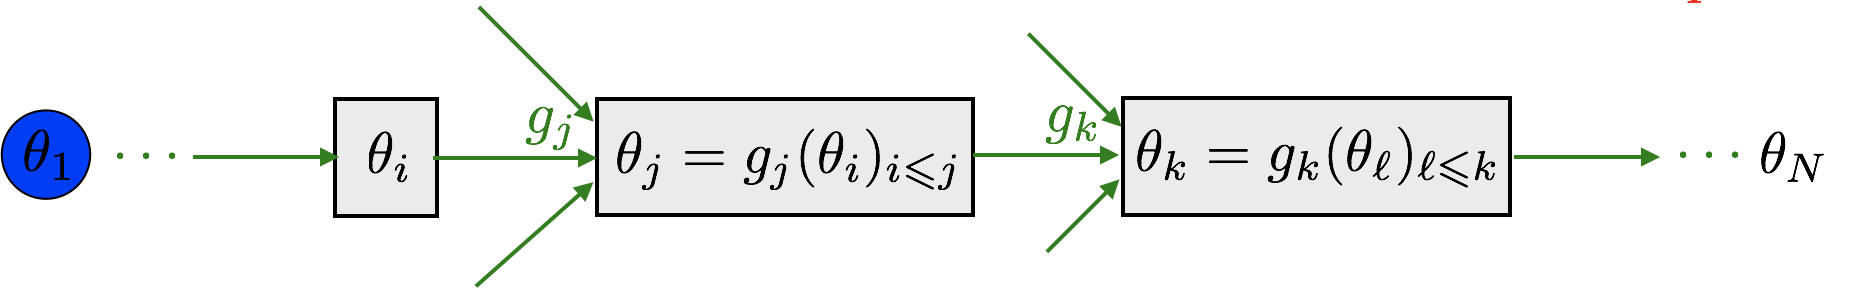
\includegraphics[width=.7\linewidth]{auto-diff/dag-element}}
\hbox{}\vspace{3mm}\hbox{}
\fbox{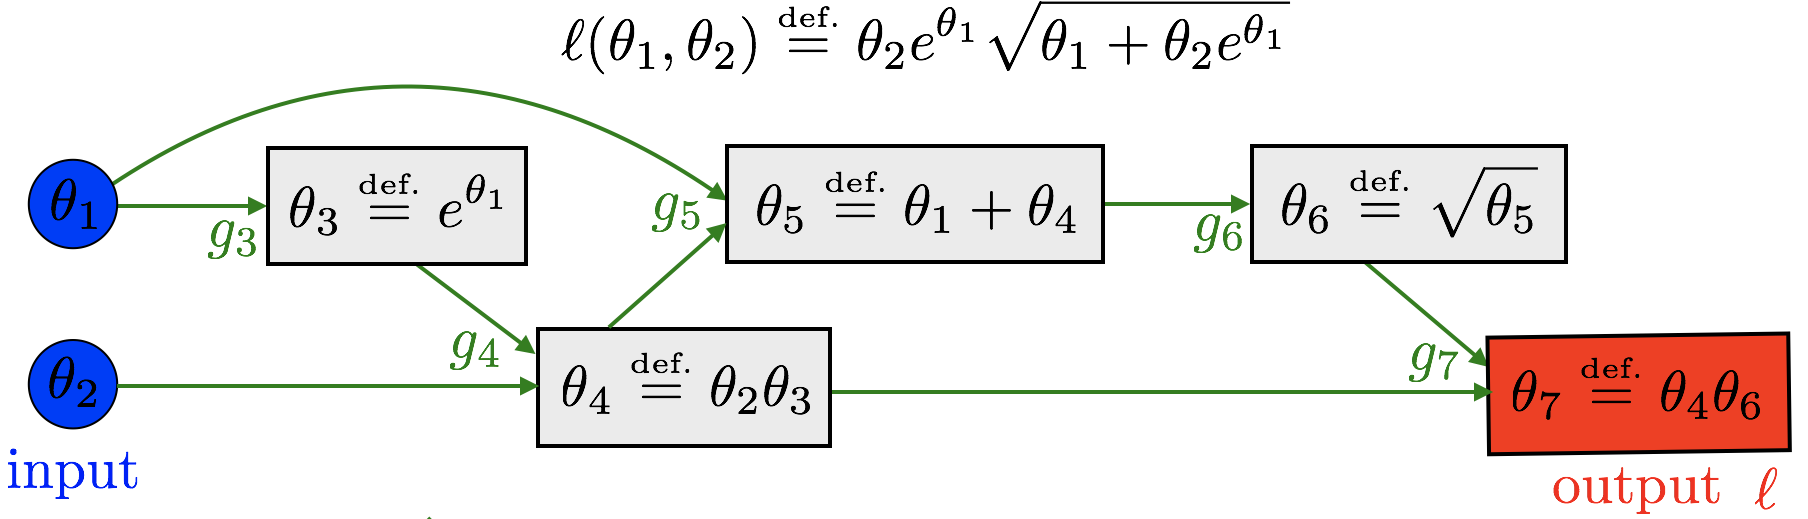
\includegraphics[width=.7\linewidth]{auto-diff/dag-example}}
\caption{\label{fig-dag-example}
Top: elementary component of the DAG computational graph. 
Bottom: example of DAG computational graph.
}
\end{figure}

One can generalize the idea above to differentiate automatically any function which can be implemented on a computer. What is even more surprising is that the computational cost is the same as the one of evaluating the function itself. This fundamental computational fact (that gradient evaluation and function evaluation have the same computational cost) is not so well known, but is of paramount practical interest when it comes to differentiating complicated recursive functions. We will apply it in a very simple setup for deep-architectures, but it can be applied to much more involved computational architectures. 

Note that this results only applies for function which output scalar values. For functions which output vector values, one can of course re-use this idea for each output, but this is in general vastly sub-optimal, because it ignore the redundancy between the computation of each output. The determination of optimal strategy in this case is known to be NP-hard. This include for instance the computation of the Hessian of a scalar valued function (since it corresponds to the differentiation of the gradient, which is itself a vector-valued function). Fortunately, for machine learning application, one is often interested in differentiating only empirical losses functions, which as scalar valued.

%%%%
\paragraph{Forward pass as a DAG traversal.}

The crux of this idea is that the computational flow of any computable function $\ell$ can be represented as a directed acyclic graph. 
%
We denote $(\th_i)_{i=1}^R$ the set of all scalar variables (input, output and intermediary) manipulated by the computational program.
%
Without loss of generality, we impose that the first variable $(\th_1,\ldots,\th_M)$ are the $M$ input variables, while the last $\th_R$ is the output variable. The function to be computed is thus of the form 
\eq{
	\th_R = \ell( \th_1,\ldots,\th_M )
}
where $\ell : \RR^M \rightarrow \RR$ is broken in $R-M+1$ intermediate steps corresponding to all the remaining variable $(\th_i)_{M < i < R}$. 
%
The successive execution of the program defines an ordering of all the intermediate variables, so that, after initializing the input variables $(\th_1,\ldots,\th_M)$, the forward pass computes the value of $\th_r$ for $r=M+1,\ldots,R$ as
\eq{
	\th_r = g_r( \th_{\pi(r)} )
}
for some scalar valued function $g_r : \RR^{|\pi(r)|} \rightarrow \RR$, where $\pi(r) \subset \{1,\ldots,r-1\}$ is the set of ``parent'' node of $r$ in a directed acyclic graph (DAG).  Figure~\ref{fig-dag-example} shows an example of such a computational DAG.


From a symbolic computation point of view, variables $\th_j$ (for $j>M$) in the graph can be interpreted either as variables (i.e. which can be assigned scalar values) and functions depending on input variables $\th_m$ for $m \leq M$. 
% 
The beauty of this DAG representation is that one can also view $\th_j$ as depending on any other intermediate variable $\th_i$ as long as $i<j$. 

%%%%
\paragraph{Direct mode auto-diff.}

The goal is to compute the gradient vector, which reads
\eq{
	\nabla \ell =  \pa{ \pd{\th_R}{\th_m} }_{m=1}^M. 
}
The naive way to comput this gradient vector would thus be to compute for each of the $M$ input variable $\th_m$ the differential $\pd{\th_j}{\th_m}$ of all function $\th_j$ with respect to $\th_m$. Without loss of generality, we consider $m=1$. This can be achieved by using the standard chain rule
\eql{\label{eq-chain-rule-forward}
	\pd{\th_j}{\th_1} = \sum_{i \in \pi(j)} \pd{\th_j}{\th_i} \pd{\th_i}{\th_1}.
}
Here the multipliers involved are actually differential of the elementary functions
\eq{
	\pd{\th_j}{\th_i} = \partial_i g_j
} 
Note that this writing is abusive, since $\pd{\th_j}{\th_i}$ really means that in practice such a differential is evaluated assuming all the variable $(\th_r)_{r<j}$ on which the function  $\th_j$ depends are defined to their respective value (which have been computed by the forward pass, which here can be run in parallel to the forward DAG traversal).

By traversing forward the DAG, iterating this formula compute all the derivative, and in particular $(\nabla \ell)_1 = \pd{\th_R}{\th_1}$. 
%
This approach, while being the most natural, is however vastly sub-optimal because its complexity is $M$ times the one of the evaluation of the function. 

%%%%
\paragraph{Reverse mode auto-diff.}

Instead of computing the quantities $(\pd{\th_j}{\th_1})_j$, a radically different approach consists in rather computing the quantities $\pd{\th_L}{\th_j} = (\nabla \ell)_j$. In place of the ``forward'' chain rule, one needs to the backward one
\eql{\label{eq-chain-rule-forward}
	\pd{\th_R}{\th_j} = \sum_{j \in \pi(k)} \pd{\th_R}{\th_k} \pd{\th_k}{\th_j}.
}
Note that here the summation is done over $k$ which are ``child'' of $j$ in the DAG. Here the multiplier appearing in the formula are differential of the elementary function since $\pd{\th_k}{\th_j} = \partial_j g_k$. 
%
The main interest of this reverse recursion~\eqref{eq-chain-rule-forward} with respect to the direct one~\eqref{eq-chain-rule-forward} is that it only needs to be run once, so that the overall complexity is the same as the one of the forward pass to compute the function itself. 

Figure~\ref{fig-fwdbwd} recaps the two passes of the reverse mode automatic differentiation method.

\begin{figure}
\centering
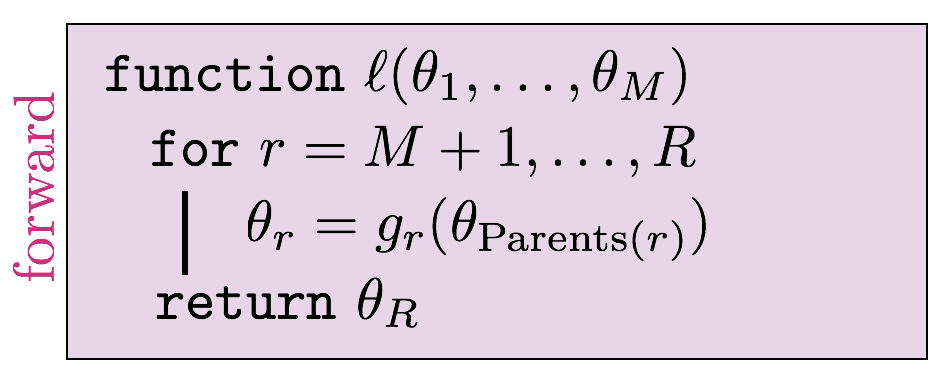
\includegraphics[width=.4\linewidth]{auto-diff/forward}
\qquad
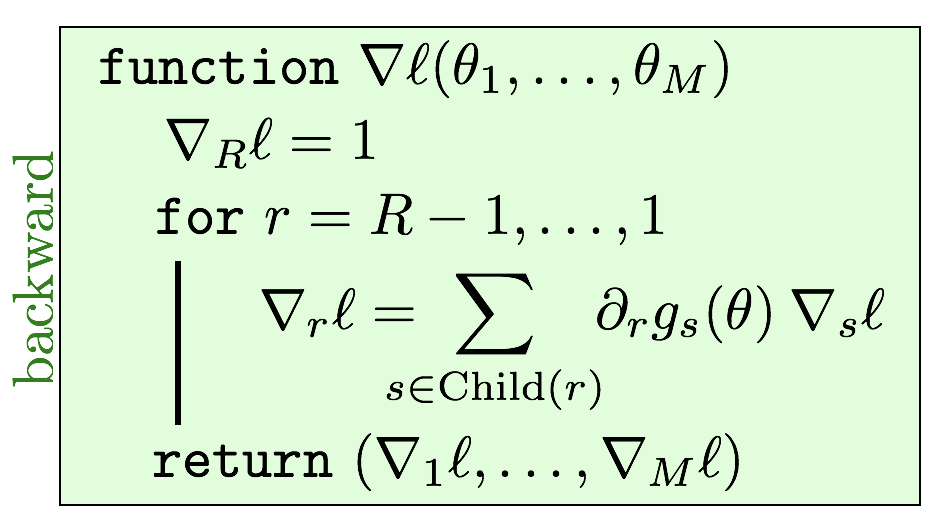
\includegraphics[width=.4\linewidth]{auto-diff/backward}
\caption{\label{fig-fwdbwd}
Recap of the two step of the automatic differentiation procedure.
}
\end{figure}

The main bottleneck of this backward automatic differentiation technic is the memory consumption. Indeed, since all intermediate results need to be computed and stored explicitly before applying the backward pass, memory grows proportionally to execution time. This can be unacceptable for very large machine learning model. Fortunately, it is possible to trade time vs. memory and only keep track of a fraction of intermediate results, and retrieve the missing result locally by small forward passes. Doing this approach recursively allows to only have a logarithmic overhead in term of both time and memory, showing the vast superiority of automatic differentiation method with respect to any other alternative for differentiation. We could not insist more on the crucial importance and impact of this class of technics on modern data science. 

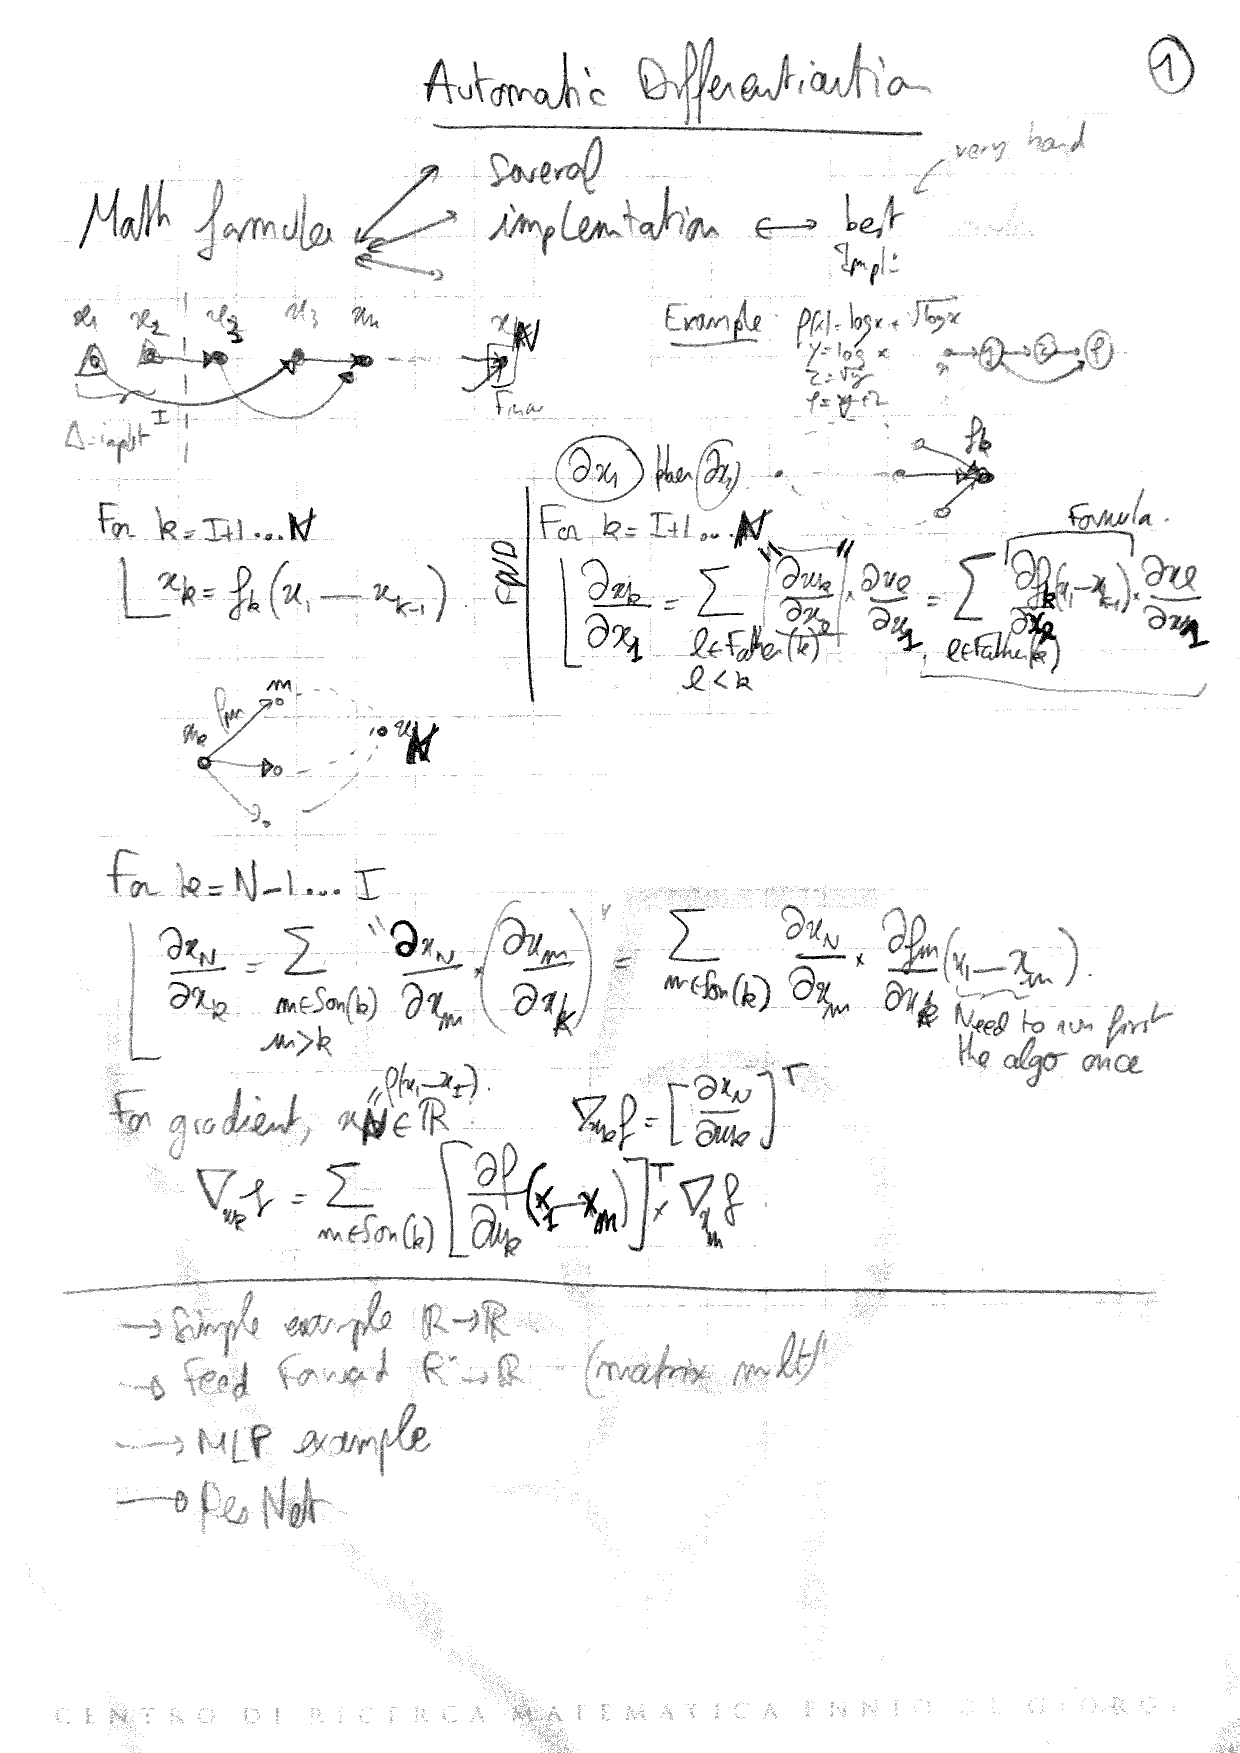
\includepdf[pages={1-},scale=1]{writing-notes/2019-11-11-autodiff-notes.pdf}

